\documentclass[]{zhawinesba} 

\title{Energy Harvesting Powered Bicycle Computer}
%\subtitle{Bachelorarbeit Elektrotechnik}
\author{Katrin Bächli,\\Manuel König}
\tutor{Prof. Dr. Marcel Meli}
\cotutor{Herr Dario Dündar}

%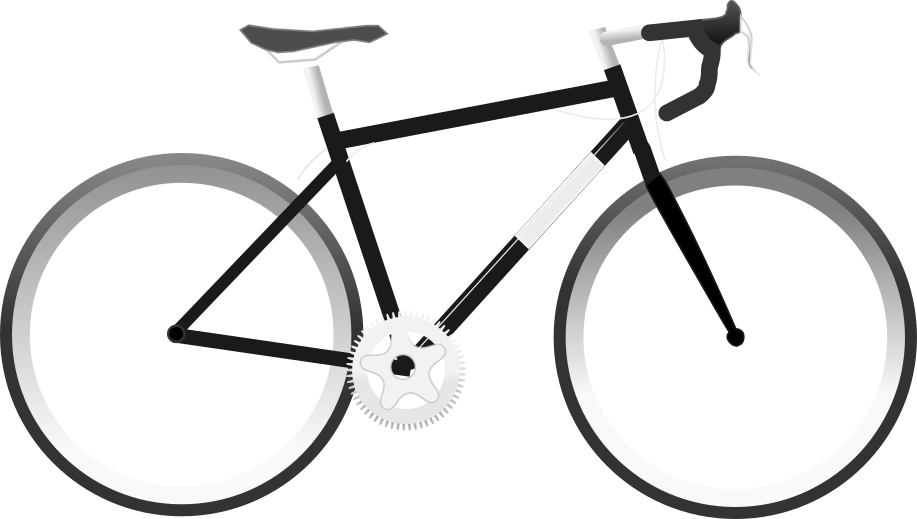
\includegraphics[scale=0.1]{0Titelblatt/road.png} 
\newcommand{\titleImagePath}{0Titelblatt/Tittelbild2.png}

%\makeatletter
%\let\oldpercent=\%
%\renewcommand{\%}{\ifmmode\oldpercent\else\thinspace\oldpercent\fi}
%\makeatother

\begin{document}


% hotfix for todos: 
% https://forum.finf.uni-hannover.de/index.php?page=Thread&threadID=10377
\setlength{\textwidth}{5.5in}    % temporär, original: 6.5in
%setlength{\evensidemargin}{1.1in} % temporär, original: 0.1in
\setlength{\marginparwidth}{3cm}  % for todos (so they don't get out of side}

%\hyphenation{20 km/h}  % no silbentrennung

\maketitle

\chapter*{Abstract}

The exchange of data between devices - commonly referred to as
\glqq Internet of things\grqq - should be made accessible to cyclists. The
mobile device should start to work at a cycling speed of 10km/h,
transmitting data through the Bluetooth Low Energy (BLE) protocol. The
task is based on a feasibility study which handles the energy
management through the chip EM8500. A \glqq SensorTag\grqq - available on Texas
Instruments Simple Link devices - is responsible for sending the data.
This board contains a wireless MCU and a low power Cortex M3.

The goal of the task was the development of a miniaturised board, which
should not be bigger than the utilized TI-SensorTag while adjusting the
energy storage, energy management and the power consumption of the
code. The finished product contains the hardware and a user friendly
Android application. The \glqq app\grqq allows adjusting the sensor readouts and
displays a tachometer and a speedometer showing the current speed, which is based on the radius of the wheel).

At the start, a feasibility study was conducted. The feasibility study
version showed promise for enough energy being produced at speeds
over 45km/h.

After improving the energy harvest we were able to generate 20
$\mu$W at 10km/h. The energy management of the EM8500-Chip and the
firmware of the TI-SensorTag were then completely rewritten. The
threshold of the energy management is based on the MPP of the harvester
and the goal is to send constant BLE-data at 10km/h. The firmware of
the TI-SensorTag uses sleep functions to reduce the energy
requirements.

The prototype is a configurable BLE-application, which sends speed,
pressure, temperature and air moisture data in 1.5 minute intervals at
10km/h. From 20km/h onward, the data is sent every 20 seconds and over
45km/h the data is sent continuously.

\chapter*{Zusammenfassung}

Internet of Things, also die Möglichkeit, Daten unter Geräten auszutauschen, soll für einen Fahrradfahrer nutzbar gemacht werden. Das  mobile Gerät soll durch Energy Harvesting gespiesen werden und bei einer Geschwindigkeit von 10 km/h Sensordaten mit Bluetooth Low Energy (BLE) senden. Die Arbeit baut auf einer Machbarkeitsstudie auf, die das Management der gewonnenen Energie mit dem Chip EM8500 löst. Als Sendemodul wird das SensorTag von Texas Instruments der Serie Simple Link benutzt. Dieses Board beinhaltet einen Wireless MCU und den Low Power Cortex M3. 

Aufgabe der Arbeit sind das Entwickeln einer minuaturisierten Leiterplatte, die nicht grösser als das verwendete TI-SensorTag ist, das Einstellen von Speicherelementen und von Schwellwerten für die Energiegewinnung und das Power optimieren des Codes. Als Produkt steht neben der Hardware eine benutzerfreundliche Android Applikation zur Verfügung. Diese beinhaltet Einstellungen der Sensoren und einen ansprechenden Tachometer, der die Fahrgeschwindigkeit anzeigt. 

Anfangs wird der Aufbau der Machbarkeitsstudie in Betrieb genommen. Die bestehende Version sendet Geschwindigkeit ab 45 km/h und basiert auf einem fliegenden Aufbau.
Nach der verbesserung der Harvesterschaltung, sodass bei 10 km/h rund 20 $\mu$W zur Verfügung stehen, wird der Print designt. Das Energiemanagment im EM8500-Chip und die Firmware des TI-SensorTags werden komplett neu geschrieben. Die Schwellwerte beim Energy Management basieren auf dem MPP des Harvesters und dem Ziel, konstant BLE-Daten bei 10 km/h zu senden. Bei der Firmware das TI-SensorTags werden über Sleep-Funktionen dem System genügend Zeit zum wieder Aufladen gegeben. 

Der Prototyp ist eine konfigurierbare BLE-Applikation, die bei 10 km/h jede 1.5 Minute Geschwindigkeits-, Druck-, Temperatur- und Luftfeuchtigkeitsdaten erhält. Bei 20 km/h werden die Daten nach 20 s und bei über 45 km/h konstant aktualisiert.

\chapter*{Vorwort}

Die Idee, Firm- und Software für einen Fahrrad-Computer zu schreiben, stammt vom Research-Assistenten vom InES, Herrn Dario Dündar. Die Themen vom Entwickeln einer Android-Applikation über das Schreiben einer Firm- und Software für einen Cortex M3 bis hin zum Layouten eines Prints sprachen uns, Manuel König und Katrin Bächli, sofort an. Ein Grund ist, dass das vorgeschlagene Projekt unsere unterschiedlichen Schwerpunkte bestens vereint, Manuel König wollte sich ins Schreiben einer Android-Applikation vertiefen und Katrin Bächli hat grosses Interesse an hardwarenaher Programmierung. 

Manuel König erarbeitete bereits in seiner Projektarbeit eine Android-Applikation und wollte das Wissen vertiefen. Auch interessierte ihn, von Grund auf eine einfache Leiterplatte zu designen. Katrin Bächli hatte generelles Interesse an Energy Harvesting und fand die Idee, ihre C-Kenntnisse durch dieses Projekt zu vertiefen verlockend. Wir wussten, dass wir auf eine funktionstüchtige Erstversion eines Fahrrad-Computers zurückgreifen konnten. Dieser wurde in einer Projektarbeit entwickelte und dient als Starthilfe. 

Während der Umsetzung des Prototypen verlagerte sich der Entwicklungsschwerpunkt zunehmend von der Software weg Richtung Hardware. Die Harvesterschaltung wird mehrfach optimiert, damit der Fahrrad-Computer schlussendlich bereits bei 10 km/h Daten an die Android-Applikation senden kann. 

Bei der Entwicklung des Fahrrad-Computers wurden wir sehr gut betreut. In gemeinsamen, wöchentlichen Sitzungen nahmen sich Prof. Dr. Marcel Meli und Research Assistent Dario Dündar Zeit. Sie setzten sich intensiv mit unseren Fragen auseinander und gaben sehr gute Vorschläge. Durch das Fachwissen konnten viele Fragen und Probleme gelöst werden. Wir lernten somit sehr viel durch diese Bachelorarbeit. 

Wir möchten Dario Dündar und Marcel Meli an dieser Stelle nochmals explizit danken. Prof. Dr. Marcel Meli kennt das Konzept des verwendeten EM8500 sehr gut und half uns, die richtigen Korrekturen vorzunehmen. Besonders in der Hardware-Entwicklung stellte er wichtige Fragen, die uns halfen, noch bessere Lösungen zu finden. Die Unterstützung durch Dario war unglaublich. Das TI-SensorTag konnte falsch reagieren wie es wollte, er gab nie auf und verhalf so, zu immer neuen Ansätzen und Lösungswegen. Ohne ihn würde der Fahrrad-Computer nicht bei 10 km/h fahren. Eine weitere wichtige Unterstützung erhielten wir durch Erich Ruff vom InES. Wir kamen beim Messen der Energie bei einer gewissen Geschwindigkeit an die Genauigkeitsgrenze. Er baute für uns einen Radimitator auf. So konnten wir genaue und reproduzierbare Messergebnisse erzielen. Weiter danken wir Herrn Blum von Delectric GmbH, welcher uns die Leiterplatten für die Arbeit kostenlos und zeitnah zur Verfügung gestellt hat. 

In dieser Projektarbeit konnte das ganze Wissen des Elektrotechnikstudiums angewendet werden: speziell vertieft worden sind die Themengebiete Elektrotechnik für die Bewegungsinduktion, Elektronik für die Schaltungoptimierung und das Leiterplatten-Design, die hardwarenahe Programmierung durch das Aufsetzen der Firmware und das Interrupt-Konzept. 

\begin{figure}[ht]
   
\includegraphics[width=0.25\textwidth]{0Vorspann/imag/delectric_logo_gross.png}
   %\caption{Delectric GmbH Logo}
   \label{delectric_logo} 
\end{figure}

Weiter danken wir Herrn Blum von Delectric GmbH, welcher uns die Leiterplatten für die Arbeit kostenlos und zeitnah zur Verfügung gestellt hat.

In dieser Projektarbeit konnte das ganze Wissen des Elektrotechnikstudiums angewendet werden. Speziell vertieft worden sind die Themengebiete Elektrotechnik für die Bewegungsinduktion, Elektronik für die Schaltungoptimierung und das Leiterplatten-Design, die hardwarenahe Programmierung durch das Aufsetzen der Firmware und das Interrupt-Konzept. 


Winterthur, 10. Juni 2016


Katrin Bächli\\
Manuel König








\addtocontents{toc}{\protect\enlargethispage{\baselineskip}} % add one line to the toc... since we don't want one more page

\tableofcontents
\chapter{Einleitung}

In einer vernetzten Welt senden Geräte Daten über ihren Zustand oder den ihrer Umgebung. Diese Technologie wird für eine Fahrradfahrerin bzw. einen Fahrradfahrer nutzbar gemacht. Das Handy soll die aktuelle Geschwindigkeit, die Höhe über Meer, die Temperatur und die Luftfeuchtigkeit während der Fahrt empfangen.

Diese Idee ist nicht neu. Erhältlich sind batteriebetriebene Modelle (siehe \ref{ausgang}), die Daten auf einem Display anzeigen. Das Neue an dieser Arbeit ist, dass die Energie aus der Fahrradumdrehung geerntet (engl. to harvest) wird und dass die Benutzerin bzw. der Benutzer sein eigenes Handy für das Anzeigen der Daten nutzen kann.


\section{Ausgangslage}
\label{ausgang}

Als Inspiration für den Prototypen dienten zwei batteriebetriebene Modelle der Hersteller Sigma Sport (\cite{SigmaSport}) und Polar (\cite{PolarElectro}). Sigma Sport bietet Geräte mit eigenem Display und  Sensoren an. Auf dem Display erscheinen neben der Geschwindigkeit die Daten der Sensoren, die GPS-Ortung und der aktuelle Ladestand der Batterie. Der Hersteller Polar stellt ein Gerät her, welches die Fahrt über GPS aufzeichnet und wichtige Informationen zur Trainingsverbesserung liefert. Jedoch wird ein (verdrahtetes) Display gebraucht.

Ein weiterer, interessanter Hersteller ist Reelight  (\cite{Reelight}). Reelight gewinnt über Wirbelströme Energie und schafft es, bei seinem Produkt City Supreme genügend Energie für eine LED-Lampe zu erzeugen. Da auf der Webseite keine Dokumentation des Funktionsprinzips erhältlich ist, ergaben eigene Untersuchungen, dass sich im Innern der Lampe ``etwas'' bewegt. Es steht zu Vermutung, dass dies ein Magnet ist, der so gelagert ist, dass er sich drehen kann. Der an der Felge vorbeiziehende Magnet erzeugt einen Wirbelstrom in der Felge. Der Wirbelstrom wirkt auf den Magneten im Fahrradlicht. Der Magnet im Fahrradlicht beginnt sich zu drehen. Befindet sich neben dem sich drehenden Magneten eine Spule, so wird genügend Spannung für das Betreiben einer LED induziert. Diese Harvesting-Methode könnte interessant für eine zukünftige Arbeit sein. Der Nachteil dieser Methode ist, dass das Erzeugen eines Wirbelstroms sich auf den Felgen bremsend auswirkt.  Bei dieser Bachelorarbeit ist die Harvesting-Methode bereits vorgegeben, da sie auf der nachfolgend genannten Projektarbeit basiert (\cite{PA_bicycle}).

Als Grundlage dient der Aufbau aus der Machbarkeitsstudie ``Bicycle computer and sensoric powered with harvested energy'' (\cite{PA_bicycle}). In dieser Projektarbeit wird der Beweis erbracht, dass durch Bewegungsinduktion genug Energie erzeugt werden kann, um die Geschwindigkeit des Fahrrads per Bluetooth Low Energy zu übermitteln. Der Aufbau funktioniert nach vorangehendem Laden der Kondensatoren zuverlässig ab 20 km/h. Das Ziel dieser Arbeit besteht aus einer verbesserten Energiegewinnung aus der Radumdrehung, einem besseren Verbrauchsmanagement bei der Datenverarbeitung durch einen Mikrokontroller und einer ansprechenden Applikation. Konkret soll ein attraktives Produkt ohne Aufladen der Kondensatoren für eine Geschwindigkeit von 10 km/h entstehen. Dieser Fahrrad-Computer-Prototyp wird in dieser Arbeit kurz Bicycle Computer genannt.



\section{Definition der Aufgabenstellung}\label{Aufgabenstellung} 

Durch die offizielle Ausschreibung der Bachelorarbeit an der ZHAW ist der Inhalt der Bachelorarbeit vorgegeben (siehe Anhang \ref{Ausschreibung}). Das Ziel der Arbeit ist es, aus dem Aufbau einer Machbarkeitsstudie einen Prototypen eines batterielosen Fahrrad-Computers zu entwickeln. Zusammen mit den Auftraggebern Prof. Dr. Marcel Meli und Herr Dario Dündar wurde die Aufgabenstellung auf folgende Anforderungen konkretisiert:

\begin{enumerate} 
	\item Die Inbetriebnahme des Vorgängermodells, das Einlesen in die vorangegangene Projektarbeit und Beschäftigung mit der Materie sind die Hauptpunkte des ersten Schrittes.
	\item Die bestehende Hardware muss verkleinert und überarbeitet werden. Dafür wird ein neues Printed Circuit Board (PCB) entworfen, welches verschiedene vorhandene Platinen vereint.
	\item Die Inbetriebnahme der Bluetooth-Schnittstelle muss auf dem Android-Endgerät und der Hardware vorgenommen werden. Eine erste Bluetooth-Kommunikation zwischen der Hardware und der Applikation ist implementiert.
	\item Das bestehende Energiemanagement soll auf die Anwendung eines Fahrradcomputers optimiert werden.
	\item Die Benutzeroberfläche der Android-Applikation soll benutzerfreundlich und optisch ansprechend gestaltet werden.
	\item Die erfassten Messwerte der Geschwindigkeit und der aktuellen Höhe sollen über Bluetooth übermittelt werden.
	\item	Die erfassten Daten sollen gespeichert und nur dann übertragen werden, wenn die nötige Energie vorhanden ist.
	\item	Per GPS soll die aktuelle Position ermittelt sowie die bereits abgefahrene Route erfasst werden. Alles soll auf einer Karte veranschaulicht werden.
	\item	Die Beschleunigung, Luftfeuchtigkeit und Temperatur sollen ebenfalls erfasst und über Bluetooth übermittelt werden.
	\item	Das Energiemanagement soll für verschiedene Geschwindigkeiten optimiert werden.
\end{enumerate}
Bei der Festlegung der Arbeitsschritte half die Vision eines innovativen Fahrradcomputers. Die Miniaturisierung, Punkt 2 in der Aufzählung oben, ist für die Attraktivität des Produkts entscheidend. Ebenso wird Vorteil dahingehend gesehen, dass das eigene Handy als Display für die Daten zu verwenden. Aus diesem Grund wurde Punkt 5 als eine der Hauptaufgaben definiert. Die App soll ansprechend und einfach für die Benutzerin oder den Benutzer sein. Das verbesserte Energy Management, Punkt 4, hat mit dem Ziel zu tun, dass der Fahrradcomputer bereits bei 10 km/h die Geschwindigkeit ausgeben soll. So gelten für die Bachelorarbeit die Punkte 1 bis 6 als Minimalanforderungen, während sich die Punkte 7 bis 10 dynamisch und in Abhängigkeit des Projektfortschritts einbauen lassen. Aus den definierten Anforderungen entstand der auf der CD abgelegte Projektplan.

\section{Übersicht der Aufgabenblöcke}

Um den Überblick der zu erledigenden Punkte zu behalten, werden die Aufgaben in Arbeitsblöcke (siehe Abbildung \ref{arbeitsbloecke}) aufgeteilt. Die Abbildung unterscheidet graphisch die oben genannten Minimalanforderungen von den den optionalen Anforderungen. Die Arbeitsblöcke mit grauem Hintergrund sind die Minimalanforderungen, die auf weissem entsprechen den optionalen Anforderungen. Die Projektplanung wurde so aufgebaut, dass bei Meilenstein 1 das Layout gezeichnet ist, bei Meilenstein 2 die Kommunikation zur App besteht und bei Meilenstein 3 die überarbeitete Version des Prototyps gezeigt wird und bis dahin die Minimalanforderungen erreicht sind. Die Arbeitsblöcke tragen eine Meilenstein-Farbe, bis wann sie erledigt sein sollen. Auf der CD im Anhang ist die Projektplanung abgelegt.


\begin{figure}[ht]
    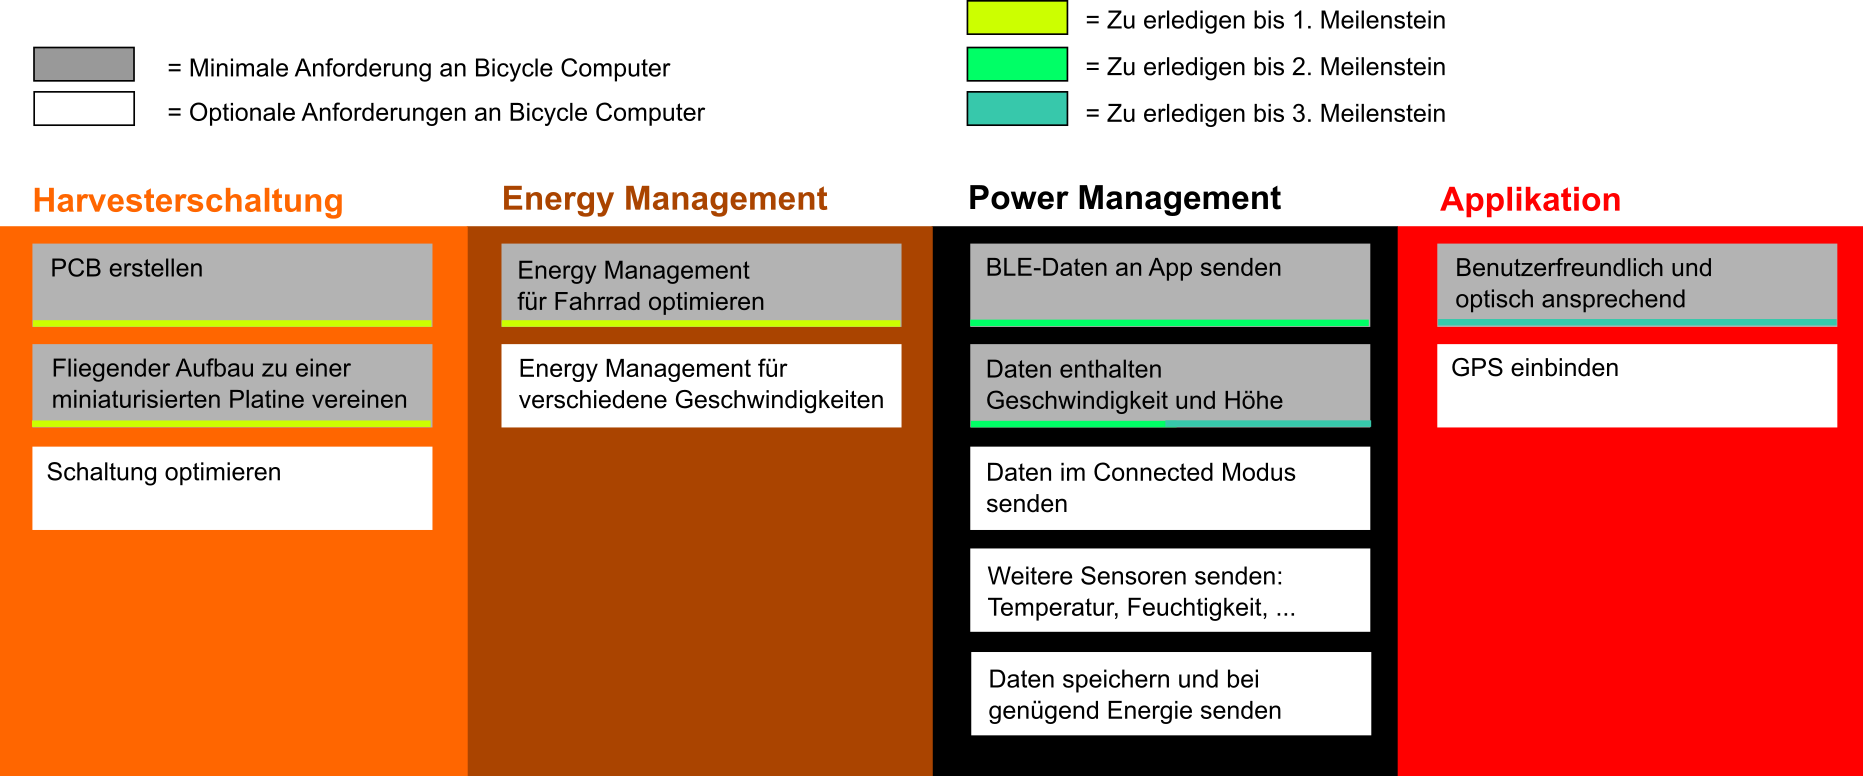
\includegraphics[width=1.0\textwidth]{1Einleitung/Arbeitsbloecke.png} 
    \caption{Arbeitsblöcke}
\end{figure}\label{arbeitsbloecke} 

\chapter{Theoretische Grundlagen}

Der Bicycle Computer basiert auf Energy Harvesting, was Energie ernten bedeutet. Welche Art von Energy Harvesting in dieser Arbeit angewandt wird, wird im ersten Unterkapitel \ref{t_harvesting} beschrieben. Im folgenden Unterkapitel \ref{t_energy_management} geht es um Ansätze zum Sammeln (engl. to accumulate) und Weiterleiten (engl. to manage) von Energie. Da die im Unterkapitel \ref{t_harvesting} beschriebene Energie im $\mu$W-Bereich liegt, ist zuerst ein Sammeln der Energie notwendig, sodass Leistungen im mW-Bereich zur Verfügung stehen. Das nächste Unterkapitel \ref{t_power_management} befasst sich mit dem notwendigen Power Management. Denn die
Energie soll nicht sofort verbraucht werden. Power Management regelt, wie schnell und wie viel Energie aufs Mal verbraucht werden soll. Als letzte Stufe in der Umsetzung ist eine energiearme Kommunikation notwendig. Bluetooth-Low-Energie-Technologie ist der Ansatz, der in dieser Arbeit verwendet wird. Das Protokoll und die Technologie werden im letzten Grundlagenteil \ref{t_ble} vorgestellt.


% 2.1-------------------------------------------------------------------
\section{Energy Harvesting}\label{t_harvesting} 

\glqq Mit Energy Harvesting [...] wird die Gewinnung von elektrischer Energie in kleinen Mengen aus dem Umfeld [...] bezeichnet.\grqq \todo{Abstand zu klein} \cite{harvesting}. Als erstes werden Methoden zur Energiegewinnung vorgestellt (\ref{harv_arten}) und danach die im Bicycle Computer verwendete Harvesting-Art genauer beschrieben (\ref{harv_bewegung}). Als letztes wird der Unterschied zwischen den unterschiedlichen Harvestingmethoden festgehalten. Denn diese Unterschiede werden in der Implementation des Bicycle Computers wichtig.


\subsection{Energy-Harvesting-Methoden}\label{harv_arten} 

Bekannte Methoden des Energy Harvesting sind die Solarzelle, die aus der Energie der Sonnenstrahlen Strom erzeugt, die Thermogeneratoren (TEG), die aus Umgebungswärme Energie gewinnen,  passive RFID-Tags, die aus der elektromagnetischen Strahlung Energie gewinnen und der piezoelektrische Effekt, der mechanischen Druck in elektrische Spannung umwandelt. Da der im Prototyp verwendete Energy-Mangement-Chip \cite{datasheet_EM85} auf die Energieoptimierung von Solarzellen oder von Thermogenaratoren spezialisiert ist, werden diese zwei Methoden vorgestellt. 


\subsubsection{Energy Harvesting mit einer Solarzelle}\label{harv_solarzelle} 

Bei der Umwandlung von elektromagnetischen Wellen (Licht) in Strom wird eine spezielle Eigenschaft des Siliziums genutzt: Führt man Silizium Energie zu, entstehen freie Ladungsträger, bzw. Elektronen und Löcher. Um aus diesen Ladungen einen elektrischen Strom zu erzeugen, ist es nötig, die erzeugten freien Ladungsträger in unterschiedliche Richtungen zu lenken; dies geschieht durch ein internes elektrisches Feld, welches durch einen p-n-Übergang erzeugt werden kann. Auf der einen Seite sammelt sich positive, auf der anderen Seite negative Ladung an. Werden diese verbunden, entsteht ein Strom (\cite{Internet_Solarzelle2}). 
Diese Harvestermethode produziert einen Gleichstrom. Grössen- und materialabhängig kann Energie im kW-Bereich gesammelt werden.

\todo{Solarstrom macht schule: Zitatfehler. Kein Jahr}

\subsubsection{Energy Harvesting mit einem TEG}\label{harv_TEG} 
TEG steht für Thermoelectric Generator und bezeichnet eine Konstruktion, die aus einem Temperaturunterschied elektrische Spannung erzeugt. Erzeugt wird die Spannung am Ende zweier metallischer Leiter aus unterschiedlichem Material, die an einem Ende verbunden sind ( \cite{Journal_TEG}). Diese Harvestermethode produziert eine Gleichspannung. Die produzierte Spannung ist vergleichsweise klein und bewegt sich im Bereich einiger 10 $\mu$V pro $1^\circ$C Temperaturdifferenz.


\subsection{Energy Harvesting über Bewegungsinduktion}\label{harv_bewegung} 
Beim Bicycle Computer wird Energie über Bewegungsinduktion gewonnen. Die Funktionsweise ist in der Machbarkeitsstudie beschrieben \cite{PA_bicycle} S.8.:

\todo{kleiner Abstand vor S. 8}

Befindet sich eine Spule in einem \textit{dynamischen} \glqq Magnetfeld\grqq, wird in der Spule eine Spannung induziert. Dies sieht man in der Formel (\ref{Formel_induzSpannung}).

\begin{equation}
    U_{ind}=-\frac{d}{dt}\intop A\,dB \ \label{Formel_induzSpannung} 
\end{equation}

Der magnetische Fluss $B$ durch die Fläche einer Spule $A$ ist gleich dem magnetischen Fluss $\phi$. Hat die Spule mehrere Wicklungen $N$, so steigt die durchflossene Fläche und mehr Spannung wird induziert. 

 
\begin{equation}
    \frac{d}{dt} \int A\,dB=\phi\cdot N\
\end{equation}

Verläuft der magnetische Fluss $\phi$ senkrecht zur Fläche der Spule $A$ kann das Integral durch eine Multiplikation ersetzt werden (siehe Formel\ref{Formelsenkrecht}). 
 
\begin{equation}
    \frac{d}{dt} \int A\,\perp\, dB=\frac{d}{dt}\int \phi\cdot N=B\cdot A\cdot N\ \label{Formelsenkrecht} 
\end{equation} 
  
 
In diesem Fall berechnet sich die induzierte Spannung in einer Spule vereinfacht mit
\begin{equation}
    U_{ind}= - N \cdot A \cdot B
\end{equation}

\todo{Bild einfügen}

Das dynamische Magnetfeld wird durch das Bewegen, oder im Fall eines Fahrrads einem Vorbeiziehen eines Magneten an einer fix verankerten Spule erzeugt.
Die produzierte Spannung hängt von folgenden vier Faktoren ab:

\begin{enumerate}
    \item die eingeschlossene Fläche $A$ der Spule    
    \item die magnetische Flussdichte des Magneten $B$ 
    \item die Anzahl Windungen $N$ der Spule und
    \item die Bewegungsgeschwindigkeit $v$ des Magneten, welche die Dauer der zeitlichen Veränderung $dt$ bestimmt
\end{enumerate}

Diese Harvestermethode produziert einen Wechselstrom, deshalb sind ein Gleichrichter und ein Kondensator zur Glättung der Rippelspannung nach der Energiegewinnung nicht notwendig. Die Leistung der produzierten Spannung geht vom $\mu$W-Bereich bis zu für die Industrie optimierten Anlagen mit Leistung MW-Bereich wie z. B. durch Drehstrom-Generatoren.



\subsection{Unterschiede Harvestermethoden}\label{harv_diff} 

\todo{Satz unverständlich!! neu schreiben. Siehe Notizen Alexey}
\todo{ gliedern in einerseits ... mit a und b  anderseits.. mit c und d}

Unterschiede zwischen den Harvesting-Methoden bestehen in der Art, in der die Energie zur Verfügung steht. Die nachfolgenden zwei Unterpunkte zeigen, dass zwei Differenzen auf: 

Punkt a verweist auf die unterschiedliche Art, in der die Energie erhältlich ist:

entspricht dies einer gleichmässigen Energie, analog zum DC, oder liefert die Quelle Energie in Form von Wechselstrom? Folgt der Strom konstant oder in Pulsen?

Die aufwendige Art \todo{unklar} der Energieerntung wird für den Prototypen relevant.  Der zweite Unterschied unter den Harvestermethoden ist die Leistungskurve. An welcher Stelle zwischen Kurzschluss \todo{unklar} und Leerlauf liegt das Leistungsmaximum? Die unterschiedlichen Leistungsmaxima der einzelnen Harvestermethoden werden unter Punkt b zusammengefasst. Beide Unterschiede werden für die Entwicklung des Prototypen über Bewegungsinduktion relevant.

\subsubsection{Gleichmässige Energie versus gepulster Energie}

\todo{Messprotokolle}

Die Solarzelle und ein TEG liefern Gleichstrom bzw. -spannung (siehe Abbildung \ref{dc}), weshalb keine Gleichrichterschaltung und Glättung notwendig sind. Die durch Bewegungsinduktion gewonnene Energie ist eine Wechselspannung (siehe Abbildung \ref{ac}, aus Messprotokoll \cite{messung_opt_spule}). Im Fall des Bicycle Computers ist diese gleichzeitig gepulst. \todo{kommender Satz umschreiben} Die Energie ist somit nicht konstant da, sondern nur in Zeitintervallen. Dadurch ergeben sich zwei Probleme bei der Energiegewinnung: 

Durch den Gleichrichter geht Energie verloren und durch die Pulsform entsteht, trotz Signalglättung über einen Kondensator, eine Rippelspannung (siehe Abbildung \ref{rippel}, aus Messsprotokoll xxxx). 

\begin{figure}[ht]
 \begin{minipage}{0.5\textwidth}
 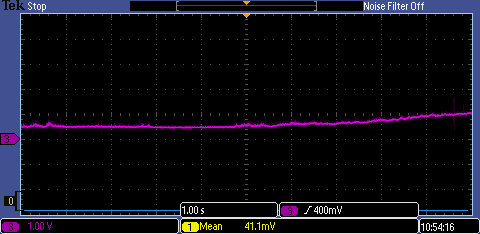
\includegraphics[width=0.9\textwidth]{2TheoretischeGrundlagen/imag/Solarstrom.PNG}
    \caption{Theoretische Abbbildung einer Gleichspannung am Ausgang eines TEG}
    \label{dc} 
 \end{minipage}
 \begin{minipage}{0.5\textwidth}
     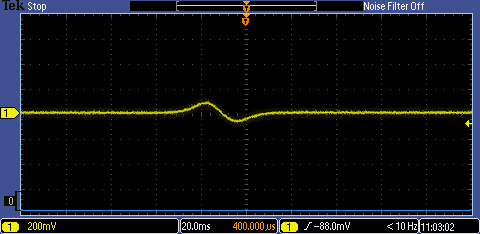
\includegraphics[width=0.9\textwidth]{2TheoretischeGrundlagen/imag/acPremospule.PNG}
    \caption{Wechselspannung bei Bewegungsinduktion}
    \label{ac} 
 \end{minipage}
\end{figure}

\begin{figure}[ht]
     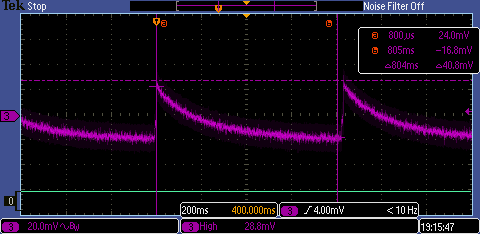
\includegraphics[width=0.45\textwidth]{2TheoretischeGrundlagen/imag/Rippel.PNG}
    \caption{Rippelspannung aufgrund der gepulsten Eingangsenergie}
    \label{rippel} 
\end{figure}



\subsubsection{Konstanter MPP zu dynamischem MPP}
\label{mpp_theorie_diff}

Die drei Harvester unterscheiden sich in ihrer Leistungskurve. 

\todo{ Erklärung der Leistungskurve} 
\todo{Erklären, was Leistungsmaximum ist} 
\todo{Übergang text neu}

Zur Verdeutlichung der Unterschiede sind für jedes Leistungsverhalten eine Abbildung angefügt. Das TEG hat unabhängig von der gewonnenen Energie und der Temperatur das Leistungsmaximum immer bei 50\thinspace\%. Die Abbildung \ref{teg} zeigt dieses unabhängige Verhalten. 


Das Leistungsmaximum, der Maximum Power Point (MPP), liegt auf der Skala von Kurzschluss bis Leerlauf proportional an unterschiedlichen Stellen.  Bei einem TEG liegt das MPP in der Mitte dieser Skala (siehe Abbildung \ref{teg}. Die MPPT-Ratio beträgt 50\thinspace\%. Bei der Solarzelle liegt das Leistungsmaximum auf der Skala bei ca. 80\thinspace\% der maximalen Spannung. Die MPP-Ratio ist 80\thinspace\% (siehe Abbildung \ref{mppsolar}). Bei der Bewegungsinduktion existiert keine fixe MPP-Ratio. Wie bei der Spule, wandert das Leistungsmaximum aufgrund mehrerer Indikatoren (wie Geschwindigkeit des Magneten durch die Spule, Abstand von Magnet und Spule) auf der Skala.



\begin{figure}[ht]
 \begin{minipage}[t]{0.5\textwidth}
 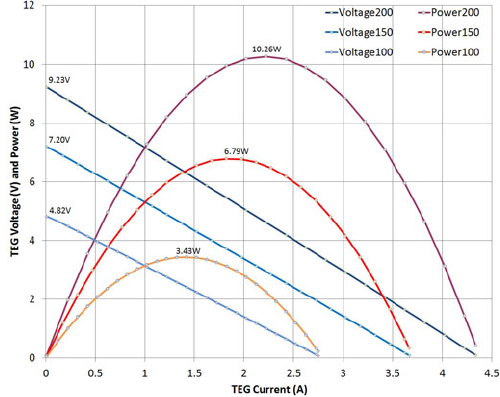
\includegraphics[width=0.9\textwidth]{2TheoretischeGrundlagen/imag/MPPTEG.png}
\caption{MPP TEG (\cite{MPP_TEG})}
\label{teg} 
 \end{minipage}
 \begin{minipage}[t]{0.5\textwidth}
    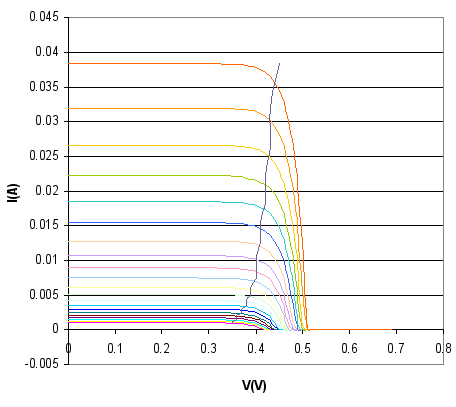
\includegraphics[width=0.9\textwidth]{2TheoretischeGrundlagen/imag/MPPSolar.png} 
    \caption{MPP Solarzelle (\cite{mpp_solar})}
    \label{mppsolar}
 \end{minipage}
\end{figure}

Abbildung \ref{mppsolar} zeigt, dass das Leistungsmaximum bei der Solarzelle unabhängig von der zur Verfügung stehenden Energie immer bei 80\thinspace\% liegt.

Die Stelle des Leistungsmaximums wandert bei einer Spule und somit bei der Bewegungsinduktion auf der Skala. Exemplarisch sind drei MPPT-Ratios einer Spule in der Abbildung \ref{bildspule} abgebildet. In dieser Abbildung zeigt sich der Einfluss des Abstands der Spule vom Magnetfeld auf die Stelle der maximalen Leistung. Diese Abbildung wurde ausgewählt, weil beim Ausmessen des Harvesters der Abstand des Magneten als einer der Einflüsse festgestellt wurde. Im Kapitel \ref{ch_resultat} Resultat sind die ausgemessenen Leistungskurven des Prototypen in der Graphik \ref{mpp_resultat_harvester} abgebildet. Die Leistungskurven wurden für verschiedene Geschwindigkeiten aufgenommen und es zeit sich, dass bei der Harvesterschaltung analog zur Spule, die MPPT-Ratio wandert. Für den theoretischen Teil wurde die MPPT-Kurven des Harverster starkt geglättet und vereinfacht (siehe untenstehende Abbildung \ref{bild_harvester}). So ist der Effekt der Verschiebung des Leistungsmaximums besser ersichtlich. Es lässt sich grob über die MPPT-Ratio des Bicycle Computers sagen, dass sie sich zwischen 35 - 75\thinspace\% bewegt.

\begin{figure}[ht]
 \begin{minipage}[t]{0.5\textwidth}
   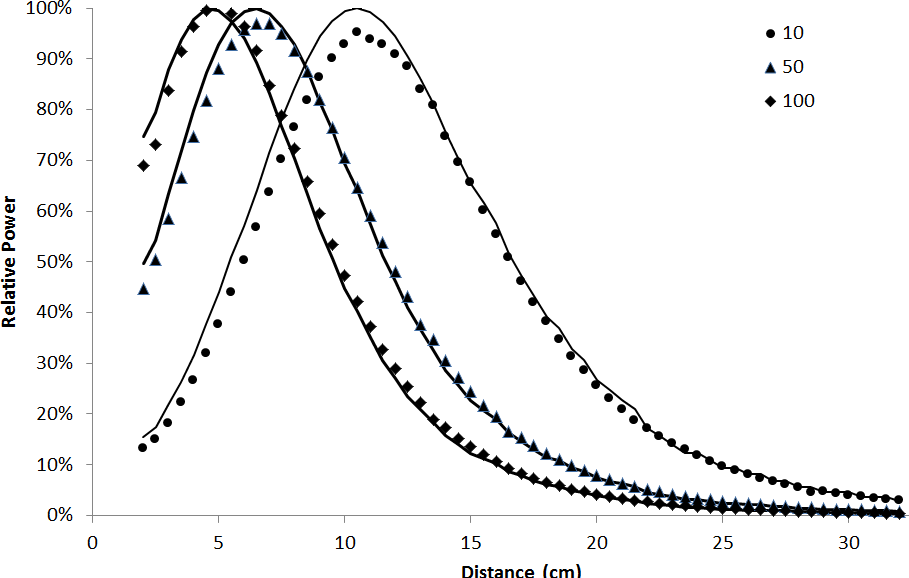
\includegraphics[width=0.9\textwidth]{2TheoretischeGrundlagen/imag/MPPSpule.png}
   \caption{MPP Spule (\cite{MPP_Spule})}
   \label{bildspule} 
 \end{minipage}
 \begin{minipage}[t]{0.5\textwidth}
   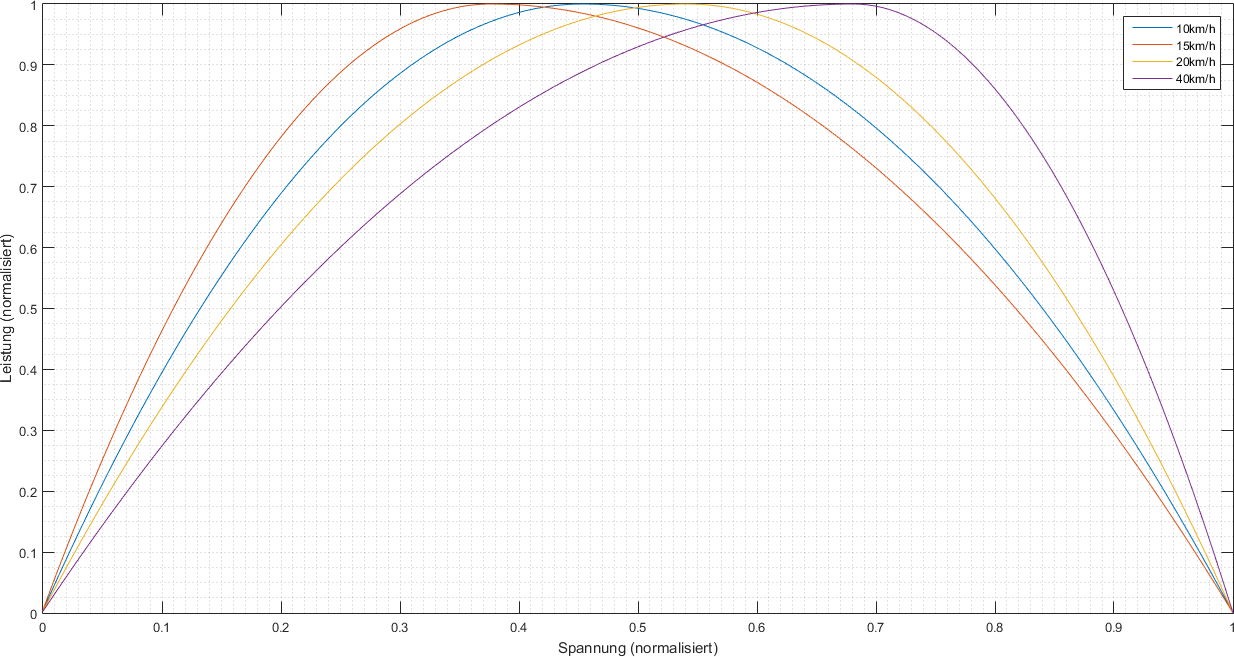
\includegraphics[width=0.9\textwidth]{2TheoretischeGrundlagen/imag/MPPharvesterTheorie.png}
   \caption{MPP Harvester (\cite{MPP_Harv})}
   \label{bild_harvester} 
 \end{minipage}
\end{figure}

% 2.2-------------------------------------------------------------------
\section{Energy Management}\label{t_energy_management} 

Der Harvester des Bicycle Computer erntet eine gepulste Energie im $\mu$J-Bereich. Um diese für eine Applikation zu verwenden, müssen die geringen Energieportionen summiert werden. Sind Energiemengen im höheren $\mu$J-Bereich verfügbar, kann die Energie kontrolliert freigegeben werden. 

Energy Management bezeichnet das Sammeln von Energie in Speichern, das Regeln des Eingangssignals auf das Leistungsmaximum und das Aufwärtswandeln von Spannung oder Strom auf einen geforderten Wert sowie die kontrollierte Freigabe der gesammelten Energie.

In der Bachelorarbeit ist das Verwenden des Chip EM8500 vorgegeben. Der EM8500 ist ein Power Management Controller für den Low Power-Bereich. Das Datenblatt des EM8500 ist der CD beigelegt.  Als erstes wird das kontrollierte Energiespeichern anhand dieses Chips erklärt. Danach folgt die Umsetzung des Maximum Power Point Trackings (MPPT) und eine kurze Erklärung der Wirkung des Boosters auf das Energy Managments. Zuletzt wird auf das Freischalten von Ausgängen eingegangen, da dies für das Verwenden der Energie die wesentliche Schnittstelle ist. 

\subsection{Kontrollierte Energiespeicherung}
\label{speicher_konzept}

Bei einer Low-Power-Harvesting-Applikation ist wesentlich, dass vor der Verwendung der Energie durch einen Microkontroller genug Energie in Speichern gesammelt wurde. Dies ist in der Abbildung \ref{em_grundprinzip} dargestellt. Sie zeigt, dass für die Freigabe der Energie an eine Applikation, erst nach dem Erreichen eines gewissen Speicherzustands erfolgt. Die Höhe des Speicherwertes kann im Register eingetragen werden. Die Ladespannung des sogenannten Primärspeichers, dem Short Time Storage (STS), ist mit VSTS in der Abbildung \ref{em_grundprinzip} abgebildet. Das Signal der Speisung der Applikation wird als VSUP bezeichnet.

\todo{ev. Blockdiagramm mit allen Bezeichnungen. oder verweis auf Graphik}

\todo{Graphik falsch: VSUP auf batminlow. vsts geht auf v bat min hi dis}
\begin{figure}[ht]
 \begin{minipage}[t]{0.5\textwidth}
   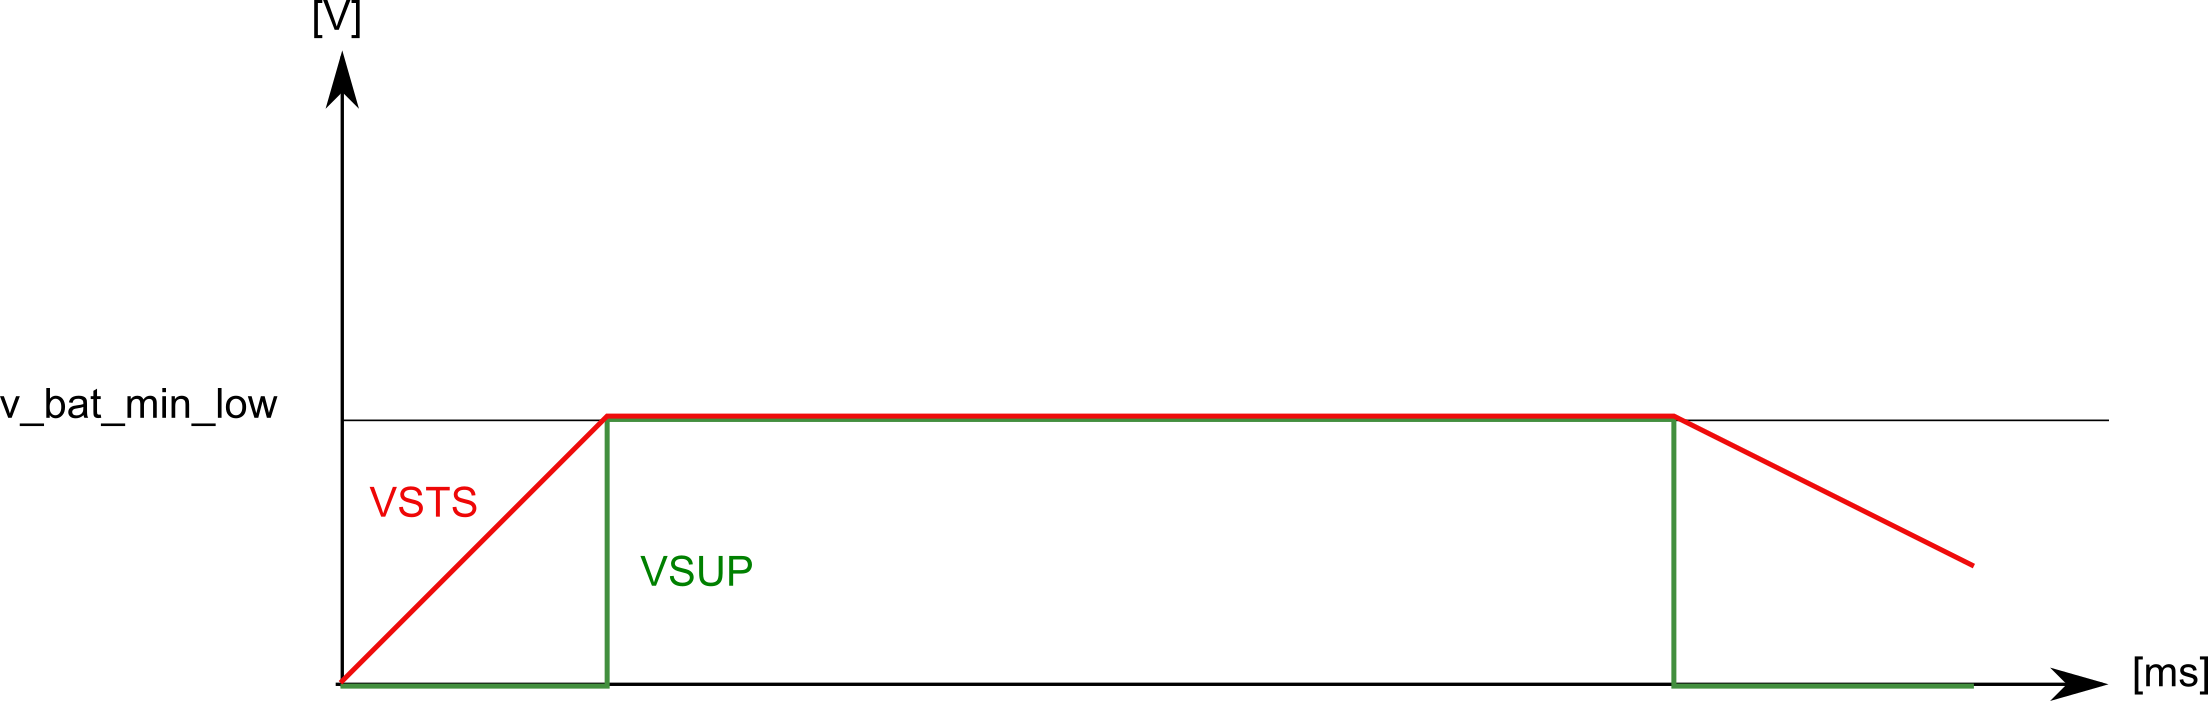
\includegraphics[width=0.9\textwidth]{2TheoretischeGrundlagen/imag/levelMitSTsTheoriel.png}
   \caption{Grundprinzip Applikationsspeisung }
   \label{em_grundprinzip} 
 \end{minipage}
 \begin{minipage}[t]{0.5\textwidth}
   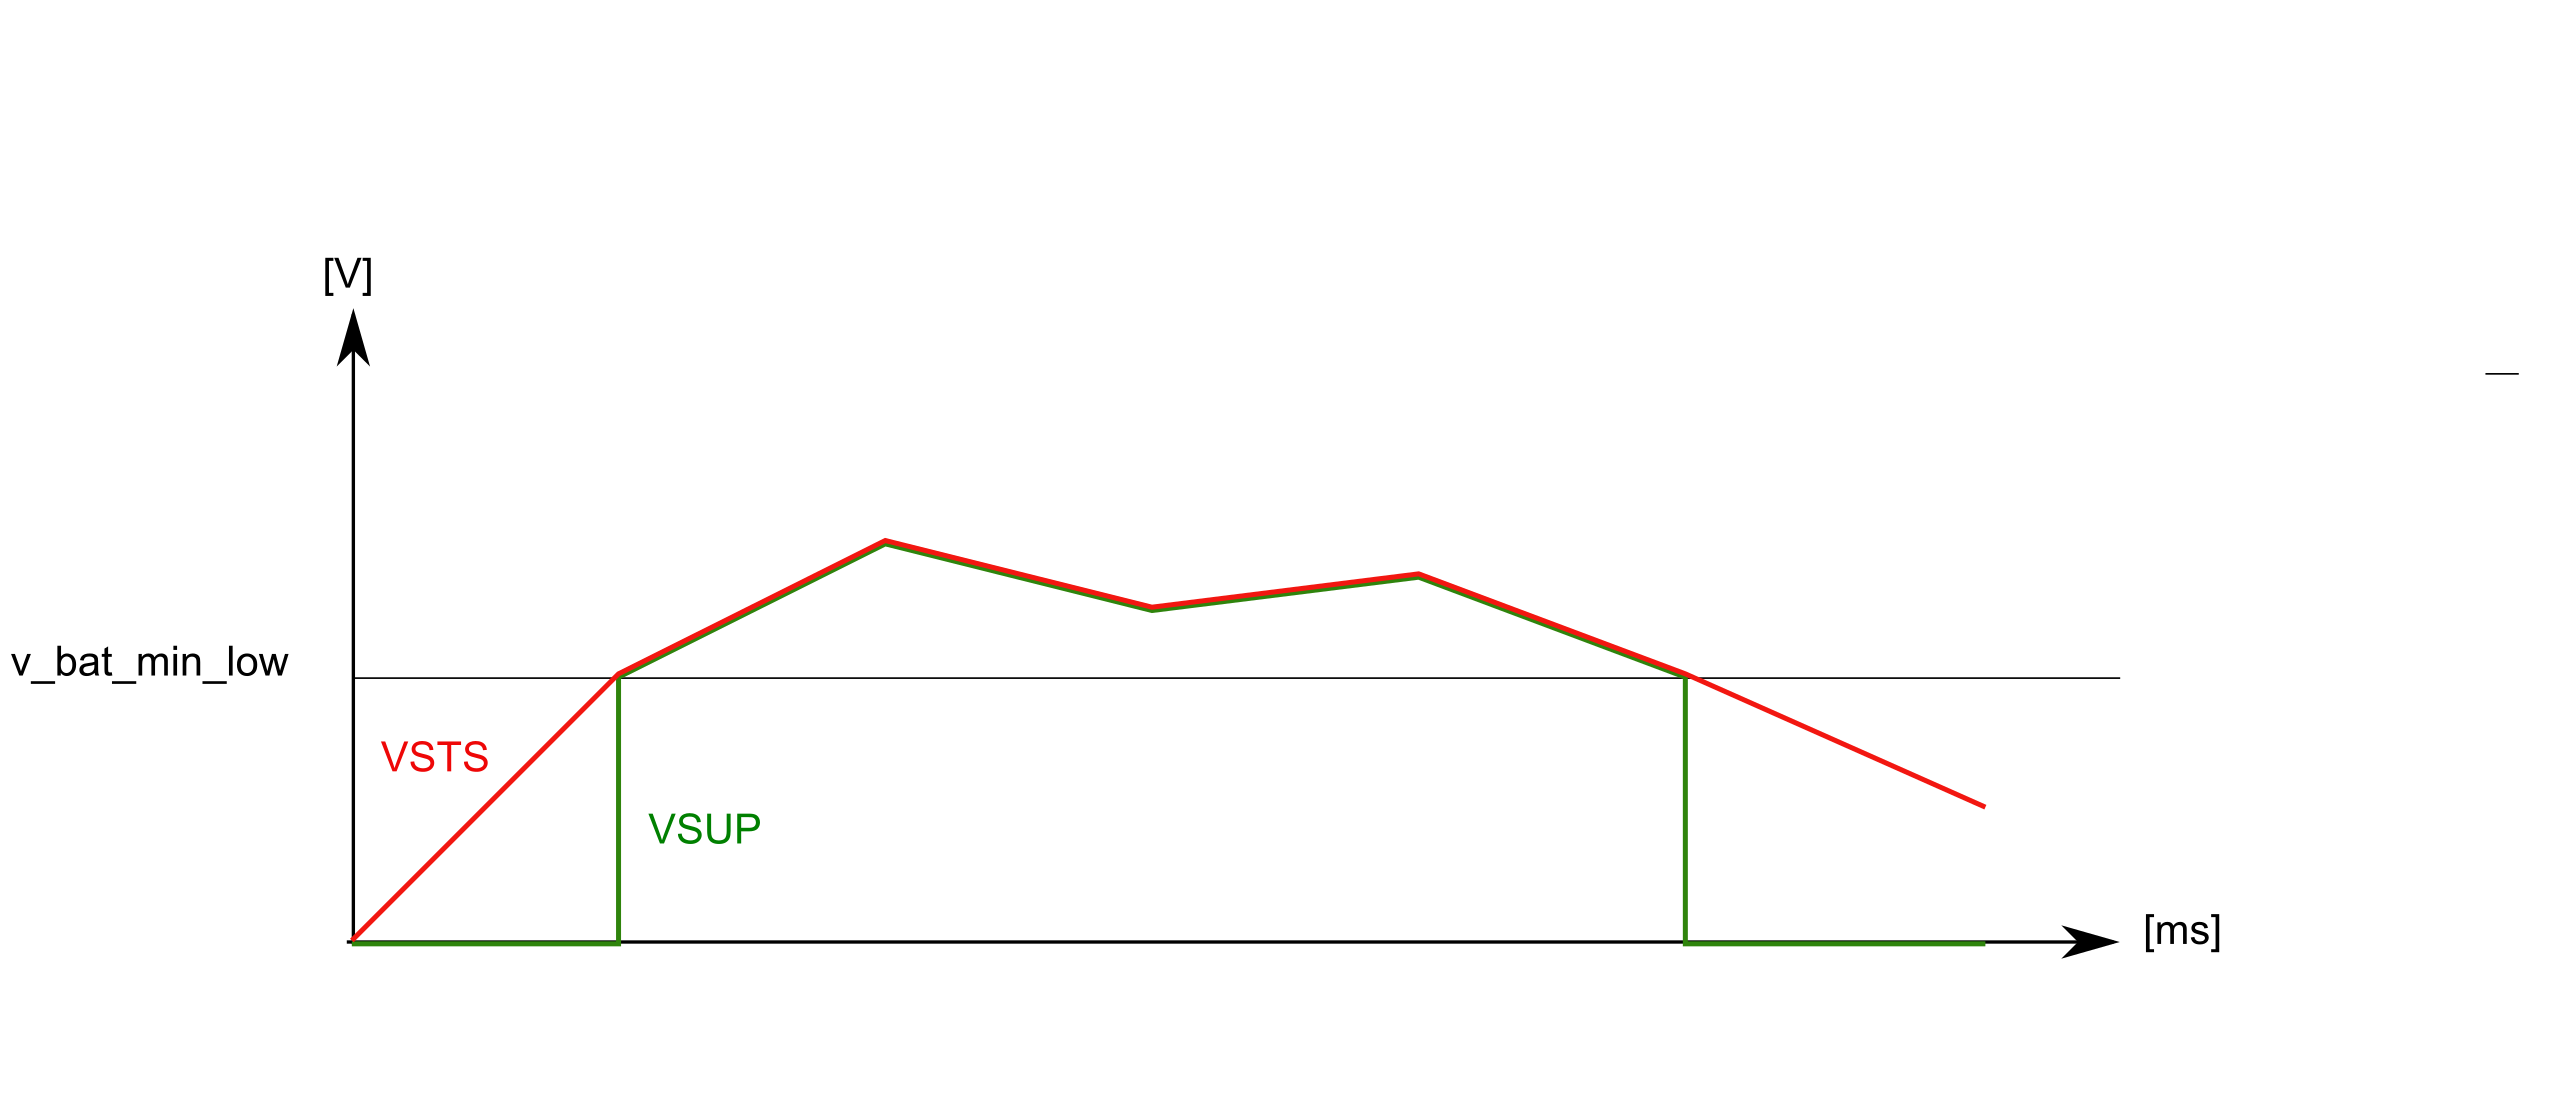
\includegraphics[width=0.9\textwidth]{2TheoretischeGrundlagen/imag/levelSTSReal.png}
   \caption{Applikationsspeisung EM8500}
   \label{em_grundprinzip_em8500} 
 \end{minipage}
\end{figure}

Im EM8500 wird dies folgendermassen umgesetzt (Abbildung \ref{em_grundprinzip_em8500}): Erreicht der Primär\-speicher STS den Schwellwert v\_bat\_min\_low, wird VSUP mit der eingestellten Spannung gespiesen. Der Registerwert v\_bat\_min\_low wird zukünftig STS\_LOW bezeichnet. Denn es ist der tiefere Schwellwert des STS, der die Spannungshöhe der Applikation definiert. Die Applikation sollte nicht alle Energie verbrauchen, sodass sich der Speicher weiter lädt. \todo{ sofort erklären warum. Denn... } VSUP folgt der Speicherspannung. Verbraucht die Applikation viel Energie, fallen VSUP und VSTS parallel. Speiste der Harvester viel Energie, steigt bei beiden die Spannung an. Unterschreitet VSTS/VSUP den Schwellwert von STS\_LOW, so wird die Speisung der Applikation gestoppt.

Der Primärspeicher STS ist für die kurzfristige Speisung der Applikation verantwortlich. So bedeutet STS Short Time Storage. Für das langfristige, sichere Ausführen braucht das System ein Long Term Storage (LTS). Seine Aufgabe ist, Reserveenergie aufzubauen. Diese überbrückt die Energieengpässe, wenn der Harvester zu wenig Energie liefert.
VLTS wird geladen, wenn der Schwellwert bei v\_appl\_max\_lo ist (siehe Abbildung \ref{energiespeisung_lts}).

\begin{figure}[ht]
 \begin{minipage}[t]{0.5\textwidth}
   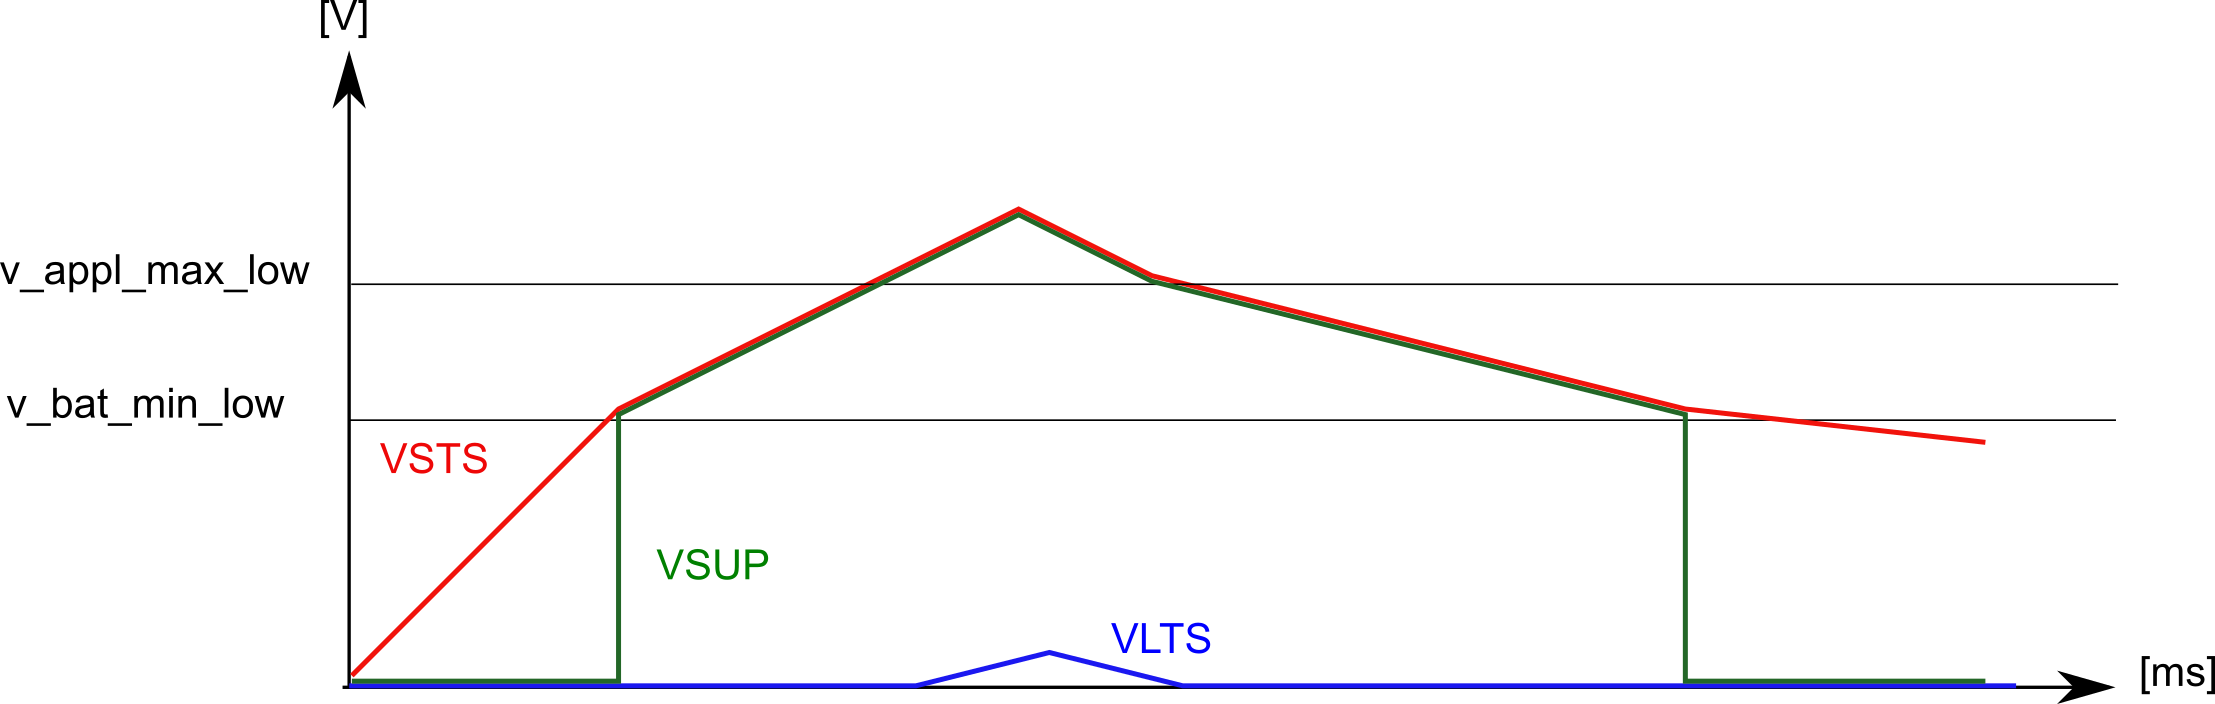
\includegraphics[width=0.9\textwidth]{2TheoretischeGrundlagen/imag/levelMitLTS.png}
   \caption{Sicheres Betreiben durch Long Term Storage}
   \label{energiespeisung_lts} 
 \end{minipage}
 \begin{minipage}[t]{0.5\textwidth}
   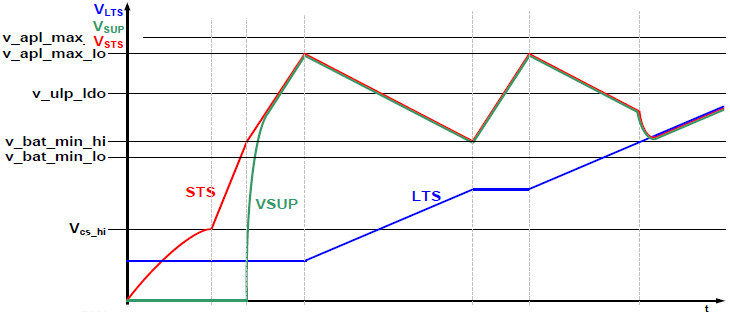
\includegraphics[width=0.9\textwidth]{2TheoretischeGrundlagen/imag/KonzeptFirma.png}
   \caption{Konzept Hersteller (\cite{datasheet_EM85})}
   \label{konzept_levels_em} 
 \end{minipage}
\end{figure}

Im Datenblatt des EM8500 (siehe \cite{datasheet_EM85}) sind weitere Feineinstellungen beschrieben und drei Application Notes helfen bei der Berechnung der Schwellwerte für ein sicheres Betreiben. Die Dateien sind auf der CD abgelegt.

Grundsätzlich ist zur Berechnung der Speicher und den Schwellwerten zu sagen, dass der erste Schwellwert (STS\_LOW), bei dem die Speisung der Applikation beginnt, genug Energie für die Initialisierung der Applikation gesammelt haben muss. Zudem muss das Abschalten von VSUP vermieden werden. Denn ein Neustart braucht aufgrund der Initialisierung viel Energie und ist ein unnötiger Kraftakt in einem Low Power System. In den Beispielkonfigurationen des Herstellers (\cite{datasheet_EM85} S. 5 - 8 ) sieht man, dass in deren Überlegungen VSUP nicht abgeschaltet wird. Der Hersteller geht davon aus, dass sogar bei dem Freischalten von VSUP die Spannung am STS nicht aufgrund der Last der Applikation fällt, sondern sich weiterhin auflädt.

\subsection{Regelung des optimalen Leistungsbezugs}
\label{optimaleLeistung}

Wichtigster Punkt in der Energieoptimierung ist, das Maximum aus der produzierten Energie weiterzuverwenden. Aus diesem Grund wird vor Inbetriebnahme eine Leistungskurve des Harvesters erstellt. Wie in Unterkapitel \ref{harv_diff} beschrieben, unterscheidet sich der Maximum Power Point (MPP) unter den Harvestern stark.

EM8500 versucht die Quelle stets in der Nähe dieses Optimums zu betreiben. Dies geschieht über eine Innenwiderstand-Regelung, sodass die Eingangsleistung möglichst dem MPP entspricht. Wie schnell die aktuelle Leistung überprüft wird, ist einstellbar. Der EM8500 besitzt eine Auflösung von 37 mV. Die Abbildung \ref{RegelungSpannung} zeigt das periodische Messen des Spannungswert des Harvesters. Da die Kurzschlussmessung für das Messen des Stromwerts eine Spannungsspitzen verursacht, (gut zu sehen in der Abbildung bei höherer Spannung), sollte die Leistungsüberprüfung nicht zu oft geschehen. Spannungsspitzen bedeuten Energieverlust, weshalb die Energiemessung nur so oft als  absolut notwendig erfolgen soll. In der Abbildung \ref{RegelungSpannung} beträgt die Periode 8 Sekunden. 

\begin{figure}[ht]
    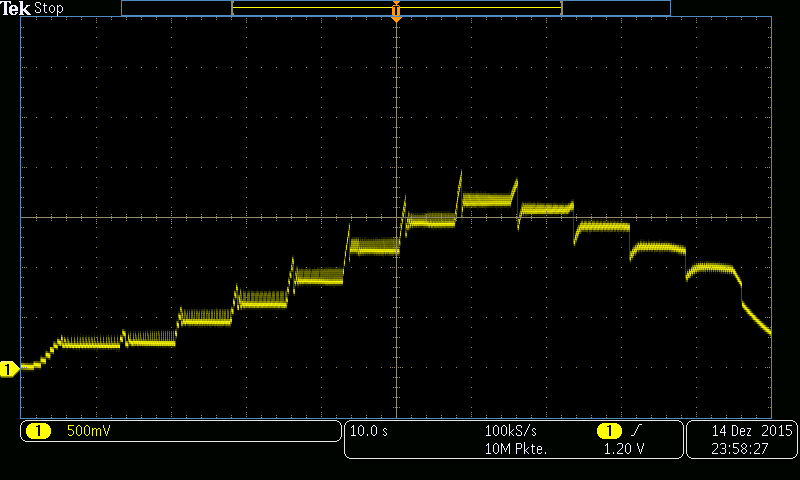
\includegraphics[width=0.5\textwidth]{2TheoretischeGrundlagen/imag/RegelungVHRV.png}
    \caption{Leistungsmessung des Harvesters}
    \label{RegelungSpannung} 
\end{figure}


\subsection{Spannung auf- und abwärtsregeln}
\label{eingangsspannung}

\todo{Titelname nicht gut} 

Beim EM8500 bilden der MPPT-Kontroller und der Booster eine Einheit (siehe Blockdiagramm im Anhang \ref{anhang_em8500}). Die Aufgabe des Boosters ist es, das interne Spannungsniveau (VREG) zu heben. Der Booster arbeitet ab einer Eingangsspannungen von 0.3 V. Danach regelt er in Schritten von 0.3 V. Der Booster geht von einer Gleichspannung eines TEG oder einer Solarzelle aus. Für diese zwei Anwendungen ist der EM8500 konzipiert (siehe \cite{datasheet_EM85}, Abschnitt Description, S. 1).


\subsection{Energiezustand kennen und In- und Ausgänge schalten}
\label{th_energiebilanz}

$E_{Applikation}$ bezeichnet die  minimale Energie, die die Applikation braucht, also mindestens die Initialisierung der Applikation. Die Applikation wird über das Signal V\_SUP, das die Energie vom Primärspeicher STS erhält, gespiesen.

\begin{equation}
  E_{Applikation}= C_{STS} \times \frac{1}{2}\, (V_{STS_LOW} )^2
\end{equation}

Da sich der Kondensator $C_{STS}$ bei der Freigabe der Energie über V\_SUP nicht auf 0 entlädt, sondern die minimale Applikationsspannung erhalten bleibt, gilt für die Berechnung des Kondensators $C_{STS}$ nur die Energiedifferenz als verwendbar. Es ist die Differenz zwischen den zwei eingestellten Primärspeicher-Schwellwerten STS\_LOW (ab diesem Schwellwert wird V\_SUP gespiesen) und  v\_bat\_min\_low (ab diesem Schwellwert hört die Speisung von V\_SUP auf). Der zweite Schwellwerte wird in der Gleichung vereinfacht als STS\_HIGH bezeichnet.

\todo{schon früher die Schwellwerte vereinfacht als STS \_HIGH,STS\_LOW bezeichnen}

\begin{flalign}\label{eq:e-high-e-low}
E_{Applikation} &= E_{STS\_HIGH} - E_{STS\_LOW}\\\nonumber
                &= C_{STS} \times \frac{1}{2}\, (V_{STS\_HIGH} )^2 - C_{STS} \times \frac{1}{2}\, (V_{STS\_LOW} )^2
\end{flalign}
%\eqref{eq:e-high-e-low} % with brackets
%\ref{eq:e-high-e-low} % look ma no  brackets

Kennt man die notwendige Energie, so kann die Grösse des Kondensator $C_{STS}$ aus der notwendigen Energie berechnet werden:

\begin{equation}
  C_{STS}= \frac{ E_{Applikation}}{(V_{STS\_HIGH} )^2 - (V_{STS\_LOW} )^2}
\end{equation}

Umgekehrt argumentiert, kann man aus der Höhe der Applikationsspannung (V\_SUP bzw. $V_{STS\_LOW}$), des bekannten Energiekonsums $E_{Applikation}$ den notwendigen Schwellwert für den Primärspeicher berechnen:

\begin{equation}
(V_{STS\_HIGH}) ^2 - (V_{STS\_LOW})^2 =  \frac{2\, \times \, E_{Applikation}}{C_{STS}}
\end{equation}


\begin{equation}
(v\_bat\_min\_low) ^2  =  \frac{2\, \times \, E_{Applikation}}{C_{STS}} + (V_{STS\_LOW})^2
\end{equation}


Neben VSUP kann per I2C oder SPI der aktuelle Spannungspegel der Regelung (VREG), die Speicher (VDD\_STS und VDD\_LTS) und des Harvestereingangs (VDD\_HRV) abgefragt werden. So kennt die Applikation jederzeit den aktuellen Energiezustand der gesammelten Energie.

EM8500 stellt zwei digitale Überwachungssignale zur Verfügung:\\ 
Der Ausgang HRV\_LOW ist auf logisch '0', wenn die Eingangsspannung vom Harvester grösser als 0.3 V ist. Fällt diese darunter, geht HRV\_LOW auf logisch '1'.
Der Ausgang BAT\_LOW zeigt die Zeitdauer an, in der nur STS die Applikation speist:

\begin{itemize}
     \item BAT\_LOW = '0'\\
           Nicht genügend Energie zur Speisung der Applikation.
           VSUP ist ausgeschaltet.
     \item BAT\_LOW = '1'\\
           Genügend Energie zur Speisung der Applikation.\\
           VSUP ist eingeschaltet.
      \item BAT\_LOW = '0'\\
           Genügend Energie zur Speisung von LTS.\\
           VSUP ist eingeschaltet.\\
           Der Zustand entspricht nicht mehr BAT\_LOW.   
\end{itemize} 

Mit den zwei digitalen Signalen kann der Energiezustand grob abgebildet werden.

\begin{figure}[ht]
    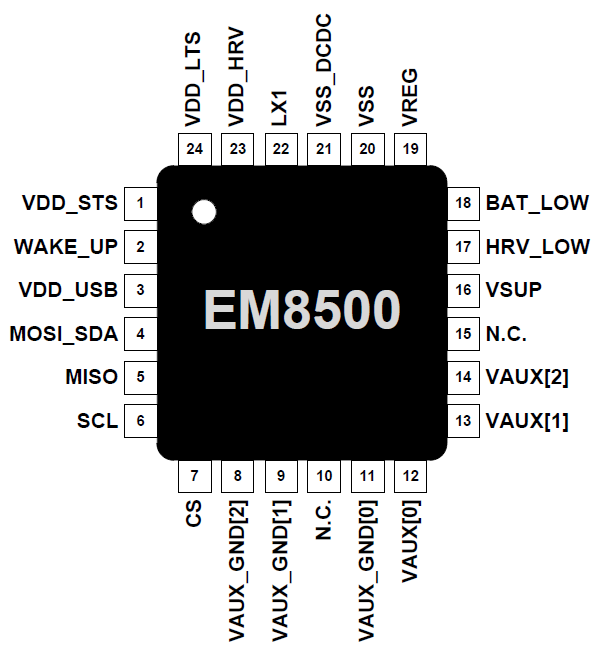
\includegraphics[width=0.5\textwidth]{2TheoretischeGrundlagen/imag/EM8500IO.png}
    \caption{In- und Outputs EM8500  (\cite{datasheet_EM85}, p.11)}
    \label{IOEM8500} 
\end{figure}



% 2.3-------------------------------------------------------

\section{Power Management}\label{t_power_management} 

Die Aufgabe des EM8500-Chip ist es, Energie zu sammeln und kontrolliert frei zu geben. Die Aufgabe das nachfolgenden Microkontrollers ist es, die freigegebenen Energieportionen optimal zu verwenden. Das bedeutet, möglichst wenig Energie bei der Datenverarbeitung zu benötigen. Dies wird durch Abstellen aller unnötigen Microkontroller-Bereiche erreicht und einem zusätzlichen Schlafen während allen Warteprozessen.

In diesem Kapitel werden zwei Ansätze zum Umsetzen eines Low Power Systems vorgestellt. Das Hauptthema ist das Schlafen zwischen allen Prozessen. Dies wird im ersten Unterkapitel beschrieben. Das Schlafen bedingt ein Aufwecken aufgrund von Ereignissen. Dadurch ergibt sich eine Interrupt Driven Applikation. Diese wird im zweiten Unterkapitel erklärt.

Vor der technischen Beschreibung der Konzepte in den drei Unterkapiteln wird kurz auf die verwendete Hardware eingegangen. In der Bachelorarbeit war als Microkontroller das Simple Link TI-SensorTag von Texas Instrument vorgegeben. Der Grund für dieses Board ist, dass das TI-SensorTag drei Anforderungen auf einem Board vereint:

\begin{minipage}{1\textwidth}
    \begin{itemize}
        \item Ein Cortex M3 dient als Haupt-Microkontroller und ist aufgrund seiner hohen, und somit schnellen, Rechenleistung und seiner Low Power-Fähigkeiten für eine Harvester-Anwendung wie der Bicycle Computer geeignet.
        \item Auf dem Board ist ein zweiter Cortex M0 für die Wireless-Anbindung angeschlossen. Dieser Prozessor kann von der Benutzerin oder dem Benutzer nicht programmiert werden, da die Schnittstelle zur Low Power Datenkommunikation fix aufgesetzt ist. Neben Bluetooth Low Energy kann auch Zigbee verwendet werden.
        \item Auf dem Board sind 10 Sensoren eingebunden.
    \end{itemize}
\end{minipage}

Die Funktionsblöcke des TI-SensorTags befinden sich im Anhang \ref{anhang_sensortag}.

\subsection{Einbauen von Schlafmodi}\label{pm_sleep} 

Low Power Microcontroller können Gebiete des Prozessors oder von Peripherieelementen temporär ausschalten. Das System befindet sich im Standby Modus. Nur die für die Applikation unabdingbaren Aktivitäten laufen mit niederstem Takt weiter. Über Interrupts können einzelne Bereiche aufgeweckt werden, die ihre Aktionen ausführen und danach geht das System wieder in den Standby Modus.

Das Verhalten, dass Prozessoren nach längerer Zeit ohne externe Input in den Schlafmodus gehen, ist typische Verhalten für Low-Power-Prozessoren. Bei einer optimierten Ultra-Low-Power-Applikation geht der Prozessor nach kleinsten Ausführungsblöcken schlafen. So gehört zum Aufwecken einer Periphierie, das Schlafen aller anderen Power Domains. Und nach dem Aufwecken der Peripherie, geht diese selbst auch wieder in den Schlafmodus. In diesem Unterkapitel werden zwei Umsetzungen des Sleep-Moduses konzeptionell erklärt.

\subsubsection{Schlafen zwischen Ausführungen}
\label{schlafen_theorie}

Die Abbildung \ref{sleep_Grundprinzip} zeigt das Grundprinzip. Das Programm besteht aus verschiedenen Aktionsblöcken. Diese dauern unterschiedlich lang und verbrauchen unterschiedlich viel Energie. Zwischen den Aktionen ist eine frei wählbare Wartezeit einbaubar ($\Delta$ t0 - t3). Die graue Markierung in jedem Aktionsblock sind die Initialisierungen vor jeder Aktion.

Während der Schlafenszeit sind alle Peripherien abgeschaltet und im Prozessor (hier als Bsp. Cortex M3) werden nur die Konfigurationen im Flash regelmässig \glqq refreshed\grqq (deutsch: neu laden). Texas Instruments entschied sich für diese Methode. Die Alternative ist, die MCU mit einem minimalen Grundpegel konstant zu speisen. Dies ist jedoch beim TI-SensorTag nicht der Fall. Texas Instruments nennt das Refreshen \glqq rentention\grqq, siehe Anhang \ref{a_powerdomain}. Die Refreshing-Peaks des TI-SensorTags sieht man im Standby-Modus. Dies ist in der Abbildung \ref{sleep_Grundprinzip} an den grünen Stromspitzen zu sehen. Ohne Refreshen des Speichers gehen die Konfigurationen verloren und vor jeder Aktion muss das System neu komplett initialisert werden.

\begin{figure}[ht]
    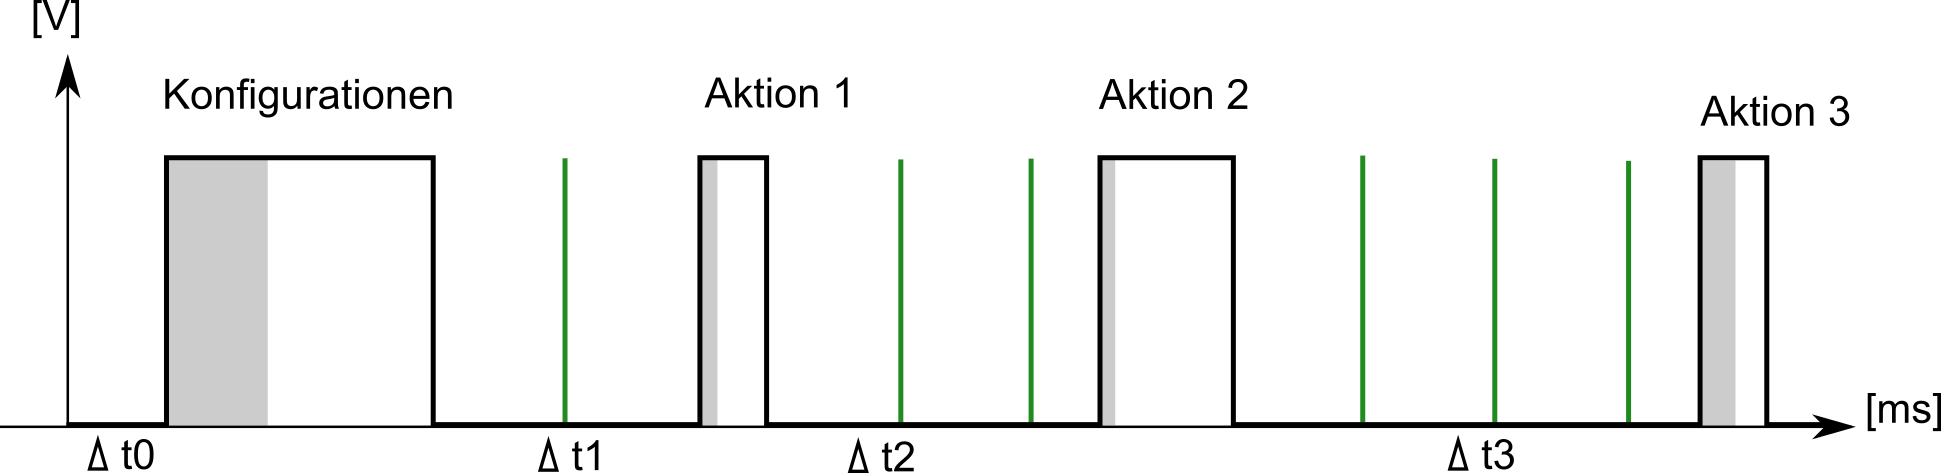
\includegraphics[width=\textwidth]{2TheoretischeGrundlagen/imag/SleepGrundprinzip.png}
    \caption{Schlafen zwischen Ausführungen}
    \label{sleep_Grundprinzip} 
\end{figure}

\subsubsection{Schlafen innerhalb einer Aktion}
Bei einer Applikation im $\mu$ - oder mW-Bereich geht das Gerät bei jedem Warteprozess, wie z.B. die Zeit, die der Sensor zum Aufwachen braucht, in den Sleep-Mode. Innerhalb des Codes dominieren die Aufwach- und Abstelleinstellungen. Für jede Aktion, wird nur die PowerDomain dieser Funktionalität eingeschaltet und nach Ausführen der Aktion wieder abgeschaltet. Die Abbildung \ref{sleep_intern} zeigt dieses Prinzip als Flussdiagramm dargestellt.

\begin{figure}[ht]
    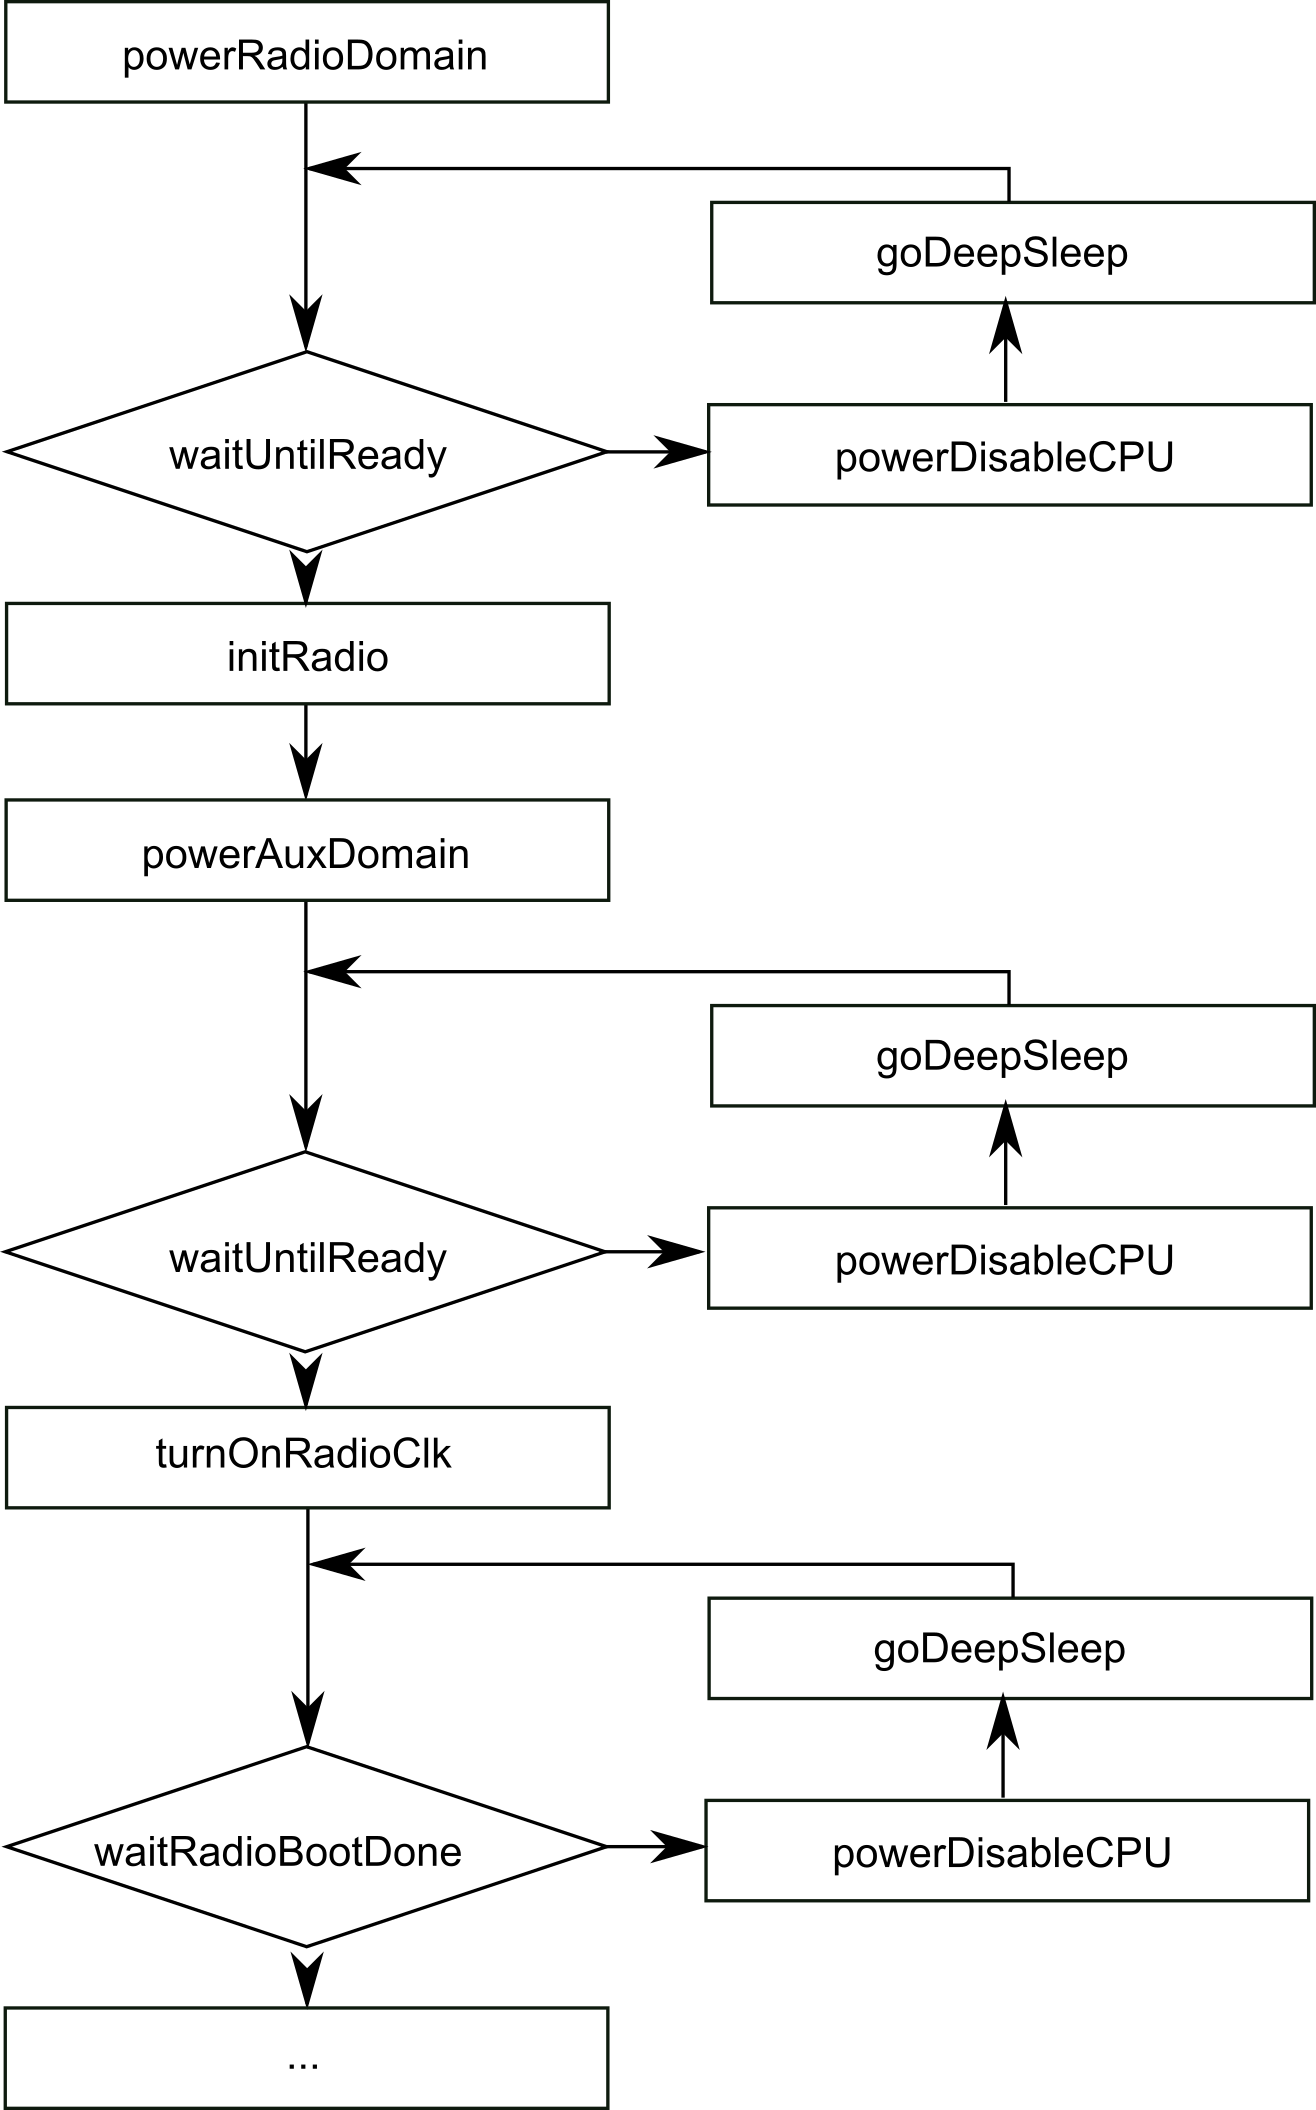
\includegraphics[width=0.5\textwidth]{2TheoretischeGrundlagen/imag/SleepInFunktion.png}
    \caption{Schlafen innerhalb des Codes}
    \label{sleep_intern} 
\end{figure}


\subsection{Interrupt Driven Application}\label{pm_interrupt}

Zum Schlafen gehört auch ein Aufwachen. Dies ist ein nicht-triviales Problem, welches sich durch Interrupts lösen lässt. In diesem Unterkapitel werden zwei Konzepte einer Interrupt Driven Applikation erklärt: fixes Aufwachen aufgrund interner Interrupts und asynchrones Aufwachen aufgrund externer Events.

\subsubsection{Aufwachen durch interne Interrupts}

Ein System kann intern seine Signale auswerten und aufgrund kombinatorischer Logik, dem Erreichen eines Schwellwertes oder dem Ablaufen eines Timers, aufwachen. Solche Wakeups sind fix und unabhängig von äusseren Einflüssen. Ein System mit internen Interrupts ist determinierbar. Das heisst, der Empfang interner Interrupts ist vorhersehbar und kann über Prioritäten geregelt werden.

\subsubsection{Aufwachen durch externe Events}

Der Prozessor, oder Teile davon, können auch aufgrund äusserer Impulse aufwachen. Die Verarbeitung des Interrupts ist dieselbe, nur weiss man nicht, wann das Ereignis auftritt. Die Gefahr, dass zwei Interrupts zur selben Zeit eintreffen oder eine Quelle mehrere Interrupts sendet, ist gegeben. Letzteres wird durch eine Entprellschaltung oder einer Entprelllösung in Software gelöst. Ansonsten können zu viele Interrupts das System absorbieren und es \glqq vehungert\grqq.

% 2.4-------------------------------------------------------------------
\section{Bluetooth Low Energy}\label{t_ble} 

Bluetooth Low Energy (BLE) bezeichnet eine Funktechnik, welche es ermöglicht, Daten zwischen Geräten auszutauschen. Der Vorteil von Bluetooth Low Energy ist der niedrigere Energieverbrauch im Gegensatz zum traditionellen Bluetooth. Das Bluetooth Low Energy Protokoll gehört zum Bluetooth Core Specification Version 4.0, wo auch das Classic Bluetooth Protokoll und das Bluetooth High Speed Protokoll enthalten sind. Die Bluetooth Core Specification Version 4.0 ist besser unter dem Namen Bluetooth Smart bekannt und wurde im Juli 2010 veröffentlicht (\cite{youtube_BLE}).

\subsection{BLE im Vergleich zu Bluetooth}
  
Bluetooth Low Energy verwendet das gleiche Frequenzband wie das traditionelle Bluetooth, jedoch sind nur 40 Kanäle \`{a} 2 MHz verfügbar, anstatt 79 Kanäle \`{a} 1 MHz beim traditionellen Bluetooth. Ausserdem verbraucht BLE, wie der Name bereits indiziert, weniger Energie als andere Übertragungsmedien. So sendet BLE mit maximal 10 mW, was einer Reichweite von ca. 10 Metern entspricht im Gegensatz zu Klasse 1 Bluetooth-Geräten, welche mit 100 mW eine Reichweite von rund 100 Metern erreichen. Ein Vorteil der BLE-Technik ist, dass die Bauteile für eine BLE-Kommunikation relativ günstig sind und damit die Geräte ebenfalls günstiger hergestellt werden können (\cite{Interent_BLE}, Abschnitt Bluetooth Range).

\subsection{Advertising und Connected Mode}

BLE wird vor allem für batterielose Sensoren verwendet, welche die Energie aus der Umwelt beziehen. Diese Sensoren arbeiten meist als Beacon, was bedeutet, dass sie Daten senden, ohne eine aktive Verbindung mit einem Gerät aufzubauen oder nur eine Verbindung auf Anfrage eingehen, diese jedoch nach kurzer Zeit wieder beenden. Dieser Modus nennt sich Advertising Mode, was vom Englischen advertisement stammt, es soll aussagen, dass der Beacon eine Werbung aussendet und diese nicht auf eine spezielle Person zugeschnitten ist, sondern an die breite Masse gesendet wird.

Eine aktive Verbindung ist bei den meisten Sensoranwendungen auch nicht notwendig, da die Daten einfach gesendet werden können und das empfangende Gerät entscheidet was mit den vorliegenden Daten gemacht wird. Wenn das Gerät mehr Informationen benötigt kann eine Verbindung aufgebaut werden. Trotzdem kann mit BLE eine aktive Verbindung eingerichtet werden, jedoch verbraucht eine aktive Verbindung mehr Energie, da Daten gesendet und empfangen werden müssen. Das bedeutet der Sensor kann nicht in einen Standby- Modus gehen, in welchem weniger Energie verbraucht wird, da auf ankommende Daten gewartet wird (\cite{BLE_advertising},\cite{ELKO_BLE}).

\subsection{BLE Pakete}

Der Aufbau eines BLE Pakets ist in Abbildung \ref{ble_paket}. Als erstes wird ein Preamble gesendet, bestehend aus abwechselnden 1 und 0, womit der Empfänger sich auf die richtige Frequenz synchronisieren kann. Diese Preamble wird auch dafür verwendet, die Verstärkung des Empfängers einzustellen. Dies kann sehr wichtig sein bei Signalen, welche von einer grösseren Distanz versendet werden, da eine falsche Verstärkung des Signals in Fehlern resultieren kann.

Anschliessend wird die Access Address verschickt, anhand dieser Adresse kann der Empfänger die Nachricht einem ganz bestimmten Sender zuordnen und somit entscheiden, ob die Daten vom richtigen Sender kommen.

Der Header enthält Informationen zum Aufbau der Daten, welche folgen. Es gibt sieben verschiedene Arten von Aufbauten der Daten.

\begin{itemize}
    \item ADV\_IND – general advertising indication
    \item ADV\_DIRECT\_IND – direct connection indication
    \item ADV\_NONCONN\_INC – nonconnectable indication
    \item ADV\_SCAN\_IND – scannable indication
    \item SCAN\_REQ – active scanning request
    \item SCAN\_RSP – active scanning response
    \item CONNECT\_REQ – connection request
\end{itemize}

Nachfolgend wird die Length eingereiht, welche Informationen über die Anzahl Bytes der Daten enthält. Es wird unterschieden zwischen der Länge eines Advertising Pakets und eines Data Pakets. Die Länge eines Advertising Pakets wird mit sechs Bits dargestellt, welche die Werte von 6 – 37 einnehmen können, wo ein Data Paket nur mit fünf Bits arbeitet, welche die Werte 0 – 31 einnehmen können.

Anschliessend werden die Nutzdaten übertragen, welche je nach gewählter Art, einen anderen Aufbau aufweisen. Es können zwischen 0 bis 296 Bits, also 0 bis 37 Bytes übertragen werden. 

Abgeschlossen wird ein Paket mit dem CRC, welcher die Checksumme der Nachricht enthält. Die Checksumme wird über den Header, Length und die Nutzdaten gebildet (\cite{BLE_Book}, Kapitel 7.2).


\begin{figure}[ht]
    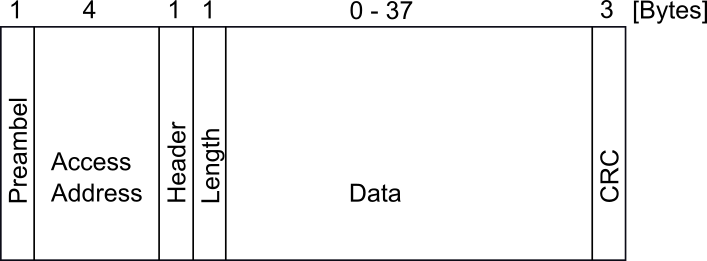
\includegraphics[width=1.0\textwidth]{2TheoretischeGrundlagen/imag/BLE_Paketstruktur.png}
    \caption{BLE Paketstruktur}
    \label{ble_paket} 
\end{figure}




\chapter{Vorgehen}
\label{ch_vorgehen} 

Das Ziel ist die Entwicklung eines Prototypen aus dem bestehenden Modell der Projektarbeit von \cite{PA_bicycle}. Die Vorgehensschritte sind in der untenstehenden Auflistung abgebildet. Sie bilden die Struktur dieses Kapitels. Die Definition der konkreten Schritte geschah in Absprache mit Prof. Dr. M. Meli und dem Resarch-Assitenten Herr Dario Dünar vom Instiute of Embedded Systems (InES). Auf der CD finden sich die Sitzungsprotokolle über den aktuellen Entwicklungsstand, die offenen Fragen und die Entscheidungen.

\subsubsection*{Liste der Arbeitsschritte}
\label{liste} 

\begin{enumerate}
  \item Inbetriebnahme Machbarkeitsstudie  
  \item Hardware entwickeln  
  \item Inbetriebnahme Prototyp      
  \item Energy und Power Management
  \item Entwickeln einer BLE-Applikation       
 \end{enumerate}  

Die sprachliche Unterscheidung von Energy- und Power-Management entspricht der Unterscheidung zweier ``Management-Teile'' im Prototypen: Das Endprodukt regelt an zwei Stellen auf unterschiedliche Art die zur Verfügung stehende Energie. Der Begriff ``Energy Management'' wird in dieser Arbeit für das Sammeln und Weiterleiten von Energie über eine Hardwareimplementation gebraucht. Der Begriff ``Power Management'' wird für die Softwareimplementation gebraucht. Diese regelt, dass die zur Verfügung gestellte Energie nicht sofort verbraucht wird. Die sprachliche Trennung ist künstlich, denn in der Umsetzung spielen Hard- und Softwareregelung Hand in Hand. Die sprachliche Unterscheidung dient der Lesbarkeit und bezeichnet keinen physikalischen Unterschied.
 
 
 % 1---------------------------------------------------------------------------
 %------------------------------------------------------------------------------
  
 
\section{Inbetriebnahme Machbarkeitsstudie}\label{v_inbetriebnahme} 

      
Ziel der Inbetriebnahme des Aufbaus der vorangehenden Arbeit von \cite{PA_bicycle} ist es, zu definieren, welche Funktionalitäten verbessert werden sollen. Zur Orientierung werden im ersten Unterkapitel \ref{fb} die Funktionsblöcke und deren Aufgaben festgehalten. Danach wird das Verhalten des Vorgängermodells in Unterkapitel \ref{verhalten} ausgemessen. Aus der Analyse entsteht die in Unterkapitel \ref{optimierung} aufgelistete erste Optimierungsliste. Als letztes folgt eine Vertiefung in das auffällige Verhalten des Eingangssignals in Unterkapitel \ref{auffaellig}.
      
\subsection{Funktionsblöcke}\label{fb} 

Der Bicycle Computer besteht aus vier Funktionsblöcken, die in der Abbildung \ref{funktionsdiagramm_bild} dargestellt sind. Der erste Funktionsblock ist der Harvester (siehe 1) in der Abbildung \ref{funktionsdiagramm_bild}). Die Aufgabe des Harvesters besteht darin, Energie zu Ernten und dem nächsten Funktionsblock (Nummer 2) in der Abbildung  \ref{funktionsdiagramm_bild} zur Verfügung zu stellen. Der zweite Funktionsblock wird als Energy Management-Teil in der Arbeit bezeichnet. Die Aufgabe des zweiten Blocks ist es, Energie zu Sammeln und kontrolliert an die Verbrauchsstelle freizuschalten. Detaillierte Informationen finden sich in den Theoretischen Grundlagen im Unterkapitel \ref{t_energy_management}. Der dritte Funktionsblock ist der Ort, an dem die Energie verbraucht wird. In dieser Arbeit dient die Energie dem Betreiben von Sensoren und dem Versenden derer Daten. Dies wird auf dem TI-SensorTag (siehe Anhang \ref{anhang_sensortag}) umgesetzt. Der Grund dafür wird in der Einleitung des Kapitels \label{t_power_management} dargelegt. Der letzte Funktionsblock bezeichnet das Ziel, das Erhalten von Sensordaten in einer Applikation.  


\begin{figure}[ht]
       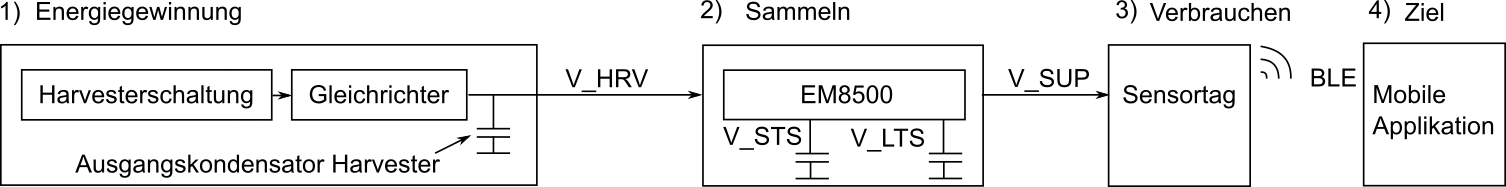
\includegraphics[width=1\textwidth]{3Vorgehen/imag/Blockdiagramm.png}
       \caption{Funktionsblöcke Bicycle Computer}
       \label{funktionsdiagramm_bild}

    \begin{tabbing}
        Bezeichnung \quad\= Beschreibung\\[0.8ex]
        V\_HRV \> Ausgangsspannung Harvesterquelle, Eingangsspannung Energy Management\\
        V\_STS\> Spannung am STS--Kondensator (Primärspeicher)\\
        V\_LTS\> Spannung am LTS--Kondensator (Sekundärspeicher)\\
        V\_SUP\> Ausgangsspannung Energy Managment, Eingangsspannung Sensortag\\
        BLE \> Senden der Daten per Bluetooth Low Energy (siehe \ref{t_ble}) \\
    \end{tabbing} 
\end{figure}

Den Funktionsblöcken sind Spannungsbezeichnungen sowie Kondensatoren beigefügt. Dies, weil bei der Beschreibung des Verhaltens des Vorgängermodells, diese Spannungslevel für die Funktionsbeurteilung wichtig werden.

  

\subsection{Verhalten des Vorgängermodells}\label{verhalten} 

Die Inbetriebnahme bestätigte das in der Dokumentation von \cite{PA_bicycle} beschriebene Verhalten. Die Abbildung \ref{spannungMachbarkeit} zeigt den zeitlichen Verlauf der Energiestände zwischen den Funktionsblöcken (siehe Abbildung \ref{funktionsdiagramm_bild}) und an den Speicherelementen. Die Legende zur Abbildung  \ref{spannungMachbarkeit} erklärt die Signale.

\begin{figure}[ht]
    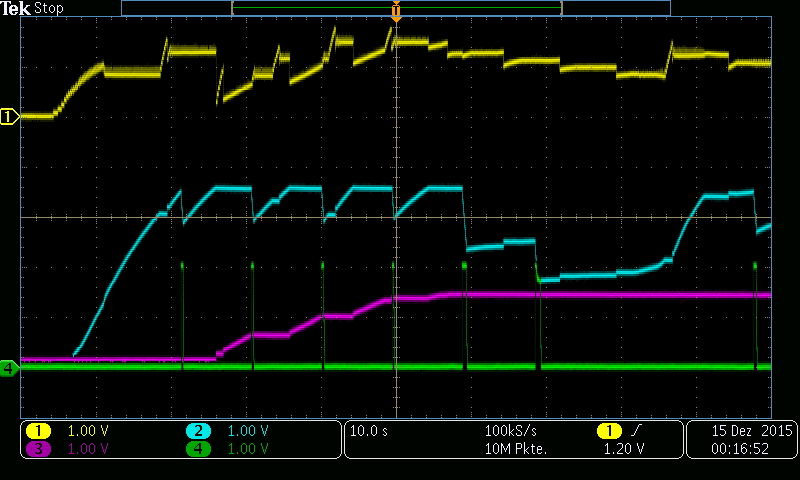
\includegraphics[width=1.0\textwidth]{3Vorgehen/imag/messungPA.png}
    \caption{Spannungswerte Modell der Machbarkeitsstudie}\label{spannungMachbarkeit} 
\begin{tabbing}
    Channel\quad\= Farbe\quad\= Beschreibung\\[0.8ex]
    CH1\> gelb\> Spannungsverlauf V\_HRV\\
    CH2\> blau\> Spannungsverlauf am STS--Kondensator\\
    CH3\> violet\> Spannungsverlauf am LTS--Kondensator\\
    CH4\> grün\> Ausgangsspannung nach Energy Management\\
     \>  \>      Eingangsspannung Sensorttag
\end{tabbing}    
\end{figure}

Im Folgenden werden die einzelnen Spannungsverläufe chronologisch entsprechend der Kanalnummer analysiert. Kanal 1 spiegelt die Spannung am Harvesterausgang wieder (V\_HRV). Gemäss Theorie \ref{eingangsspannung} bzw. gemäss Datenblatt des EM8500 ist der EM8500-Chip für ein DC-Signal ausgelegt. Er geht von einem regelmässigen Eingangssignal aus und regelt die Spannung auf den MPP. Diese Regelung sollte wie in Abbildung \ref{RegelungSpannung} aussehen. Das reale Signal entspricht nicht diesem Verhalten. Die Regelung ist abrupt und überspringt mehrere Spannungslevel. Der Ursache für die schlechte Regelung soll nachgegangen werden.

Kanal 2, blau, gibt den Spannungsverlauf am Hauptspeicher, dem Primärspeicher, der im Datenblatt von EM8500 STS heisst, wieder. Das Energy Management des Vorgängermodells setzt den Schwellwert für den Primärspeicher (STS) mit 3.6 V hoch an. Details zu den Schwellwerten sind im Kapitel Theoretische Grundlagen \ref{t_energy_management} zu finden. Der hohe Wert erklärt sich durch das Ziel, genug Energie für ein konstantes Paketversenden zu haben. Dies gelingt für fünf BLE-Pakete. Danach reicht die Energie nicht mehr aus. V\_SUP, grünes Signal, wird nicht mehr gespiesen. Nach 30 s ohne Pakete senden ist wieder genug Energie für weitere 5 Datenpakete gespeichert.

In der Auswertung fiel uns auf, dass dieser Signalverlauf nur bei einer Geschwindigkeit von 45 km/h möglich ist. Die Speicherkapazität von 470 $\mu$F und ein Schwellwert der Spannung von 3.6 V ist mit normaler Geschwindigkeit (10 km/h) nach 30 min nicht zu erreichen. Fährt man rund 45 km/h so erhält man die in der Abbildung \ref{spannungMachbarkeit} gezeigte Ladezeit von rund 25 s. Eine exakte Geschwindigkeitsmessung ist zu Beginn der Arbeit nicht möglich. Das Rad wird von Hand gedreht und mit einem Metronom wird die Umdrehungsgeschwindigkeit vorgegeben. Bei einem Radumfang von 2.04 m und einer Zeitdifferenz von 160 ms zwischen den Reed-Impulsen, ergibt sich die Geschwindigkeit von ca. 45 km/h. Da diese Messmethode über längere Zeit nicht sehr genau ist, bestand eine der Aufgaben nach der Inbetriebnahme im Organisieren eines Messaufbaus. Dieser professionellere Messaufbau wird im Anhang \ref{messaufbau} beschrieben.

Kanal 3, das rosa Signal, zeigt die Spannung am Long-Time-Speicher. Die Inbetriebnahme zeigt, dass sich der LTS lädt. Es erstaunt jedoch, dass seine geerntete Energie nicht verwendet wird. Der Spannungswert von LTS geht nie herunter.
Die Vermutung ist, dass der eingestellte Schwellwert für den Bezug von Energie von LTS (siehe Abbildung \ref{energiespeisung_lts}) nicht stimmt.

Kanal 4, das grüne Signal zeigt die Speisung des TI-SensorTags. Im Modell der Projektarbeit steuert der Mikrokontroller des Sensortags den Verbrauch. Alle 10 s wacht das System auf, bezieht Energie vom EM8500-Ausgang für das Senden eines Paketes und geht dann wieder schlafen. Das Aufwachintervall ist fix.


\subsection{Optimierungsliste}\label{optimierung} 

Aus den Messungen der Inbetriebnahme konkretisierten sich die generellen Aufgaben, die in der ersten Liste der Arbeitsschritte zu Beginn des Vorgehens  beschrieben wurden. Nachfolgende vier Punkte sollen durch den Prototypen verbessert werden: 

\begin{minipage}{1\textwidth}
\begin{itemize}
     \item Der Verlauf des Harvester-Eingangs wechselt abrupt. Der Eingang soll besser geregelt werden. 
     \item Für das Laden des Primärspeichers von 470 $\mu$F in 25 s benötigt es eine Geschwindigkeit von mehr als 60 km/h.  Die Harvesterschaltung soll so weiterentwickelt werden, dass bei 10 km/h genug Energie zum Senden von BLE-Paketen besteht.    
     \item Das zweite Speicherelement, der LTS, entlädt sich nicht. Dadurch kann seine Energie nicht verwendet werden. Die Schwellwerte am EM8500 und ev. die Kondensatorenwerte sollen so angepasst werden, dass sich der zweite Kondensator entlädt
     \item Die Energie wird statisch nach einem fixen Zeitintervall von 10 s genutzt. Das Zeitintervall soll der Geschwindigkeit angepasst werden. Bei höherer Geschwindigkeit soll das Intervall kürzer werden.
\end{itemize} 
\end{minipage}

Im Resultatsteil Kapitel \ref{ch_resultat} werden die Fortschritte in diesen vier Punkten ausgewiesen.

\subsection{Vertiefung Harvesterausgang}\label{auffaellig} 

Herr Ives Théoduloz hatte uns im Rahmen eines Besuchs auf die Problematik, einer zu grossen Kapazität am Eingang des EM-Chips, hingewiesen. Laut seiner Aussage sollte der Kondensator am Eingang des EM-Chips, bzw. dem Ausgang des Harvesters am besten kleiner sein als 4.7 $\mu$F. Bisher wurde im Aufbau der Machbarkeitsstudie ein Kondensator mit 470 $\mu$F verwendet. Herr Ives Théoduloz meinte, dass dieser Kondensator viel zu gross sei und dass die Regelung am Eingang des EM-Chips möglicherweise nicht richtig funktionieren würde. Daher wurde dieses Problem näher untersucht und in mehreren Schritten optimiert.

Im ersten Schritt wurde der Kondensator verkleinert, bis die Rippelspannung noch annehmbar war. Die Rippelspannung bei dem bestehenden Kondensator von 470 $\mu$F beträgt ca. 10 mVpp. Die Rippelspannung bei einer Kapazität von 47 $\mu$F beträgt bereits ca. 40 mVpp, jedoch ist die Rippelspannung noch in einem Bereich der annehmbar scheint. Bei einer Kapazität von 10 $\mu$F liegt die Rippelspannung bei ca. 500 mVpp. Die Abbildung \ref{47uF_mit_Limiter_AC} veranschaulicht die Rippelspannung von einem Kondensator mit 47 $\mu$F, die Abbildung \ref{10uF_mit_Limiter_DC} zeigt die Rippelspannung über einem Kondensator von 10 $\mu$F.

\begin{figure}[ht]
 \begin{minipage}[t]{0.5\textwidth}
    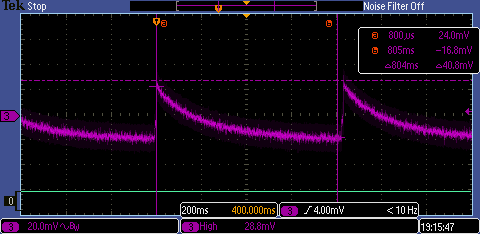
\includegraphics[width=0.90\textwidth]{3Vorgehen/imag/47uF_mit_Limiter_AC.PNG}
    \caption{Rippelspannung über dem 47 $\mu$F Kondensator}
	\label{47uF_mit_Limiter_AC} 
 \end{minipage}
 \begin{minipage}[t]{0.5\textwidth}
    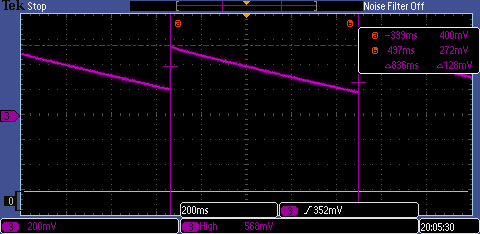
\includegraphics[width=0.90\textwidth]{3Vorgehen/imag/10uF_mit_Limiter_DC.PNG}
    \caption{Rippelspannung über dem 10 $\mu$F Kondensator}
	\label{10uF_mit_Limiter_DC} 
 \end{minipage}
\end{figure}

Jedoch muss auch ein Blick auf die Spannung am Harvesterausgang geworfen werden, wenn dieser Ausgang mit dem EM-Chip belastet wird. Es kann beobachtet werden, dass der Eingang des EM-Chips ein fluktuierendes Spannungslevel (siehe Abbildung \ref{VCC_47uF_15kmh_Periode}) erhält. 

\begin{figure}[ht]
   \begin{minipage}[t]{0.5\textwidth}
     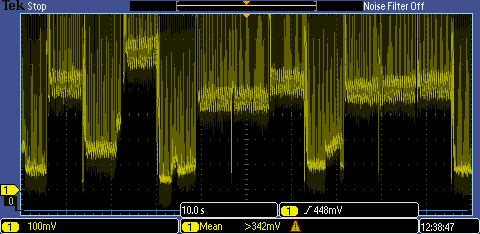
\includegraphics[width=0.90\textwidth]{3Vorgehen/imag/VCC_47uF_15kmh_Periode.PNG}
     \caption{Spannung am EM8500-Eingang über einem 47 $\mu$F Kondensator}
	 \label{VCC_47uF_15kmh_Periode}
  \end{minipage}
  \begin{minipage}[t]{0.5\textwidth}
    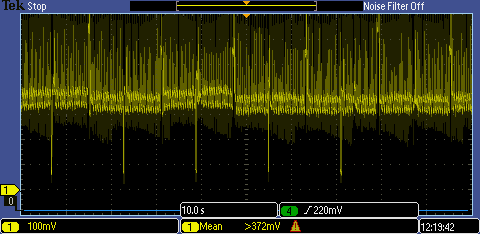
\includegraphics[width=0.90\textwidth]{3Vorgehen/imag/VCC_100uF_15kmh_Periode.PNG}
    \caption{Spannung am EM8500-Eingang über einem 100 $\mu$F Kondensator}
	\label{VCC_100uF_15kmh_Periode}
  \end{minipage} 
\end{figure}

Problematisch ist, dass die Spannung am Eingang des EM8500-Chip wiederholt unter die 0.3 V Grenze fällt, bei einer Spannung von 0.3 V kann keine Energie gespeichert werden. Die Regelung am Eingang des EM-Chips kann mit der anliegenden Rippelspannung nicht richtig arbeiten. Die Rippelspannung muss verringert werden, bzw. die Kapazität am Ausgang des Harvesters muss erhöht werden. 

Das Problem ist, dass durch den Rippel die periodische Open-Loop-Spannungsmessung keine korrekten Messwerte erhält. Sobald die Last vom Harvesterausgang abgehängt wird, steigt die Spannung über dem Kondensator, jedoch wird die Open-Loop-Spannung bei einer grossen Kapazität nicht erreicht, da die Zeit, bis der Kondensator komplett geladen ist, sehr gross ist. Jedoch bedeutet eine niedrige Kapazität, dass die Rippelspannung relativ hoch ist und je nach Zeitpunkt der Open-Loop-Messung eine andere Spannung am Kondensator ergibt. Die Spannung am Kondensator steigt bei jeder Messung auf ein anderes Spannungslevel.

Es musste ein Kompromiss gefunden werden, so dass die Spannung am Eingang des EM-Chips auf ein konstantes Level geregelt werden kann. Die Kapazität des Kondensators sollte nicht zu klein sein, damit der Rippel nicht zu gross wird. Andererseits darf der Kondensator nicht zu gross sein, da ansonsten die Open-Loop-Messung keine richtigen Werte liefert. Den Kompromiss stellt der 100 $\mu$F Kondensator dar, bei diesem ist die Spannung am Eingang relativ konstant und es kann damit gearbeitet werden (siehe Abbildung \ref{VCC_100uF_15kmh_Periode}).

Aus den Beobachtungen ergaben sich folgende Aufgaben für die Entwicklung des Prototypen:

\begin{enumerate}
    \item Die Harvesterschaltung funktioniert nicht optimal. Die Auswirkung des zu hohen Kondensator vor Harvestereingang soll getestet werden
    \item Die Schaltung soll für eine Geschwindigkeit von 10 km/h ausgelegt werden
    \item Die Konfigurationen beim EM8500 sollen überarbeitet werden, sodass LTS genutzt wird
    \item Das Senden der Pakte soll der Geschwindigkeit angepasst werden
\end{enumerate}

Punkte 1 und 2 haben Auswirkung auf das Layout, Punkte 3 und 4 auf die Entwicklung des Energymanagements und der Firmware für das TI-SensorTag.


%------------------------------------------------------------------------------
% 2---------------------------------------------------------------------------
%------------------------------------------------------------------------------



\section{Hardware entwickeln}

Aus der Inbetriebnahme der Machbarkeitsstudie wurden einige Punkte ersichtlich, welche mit einer neuen Leiterplatte, bzw. einer neuen Hardware verbessert werden können. Im speziellen muss die Harvesterschaltung genauer angeschaut werden und es soll versucht werden, die nachfolgenden Punkte aus der Inbetriebnahme der Machbarkeitsstudie umzusetzen. 

\textit{Die Schaltung soll für eine Geschwindigkeit von 10 km/h ausgelegt werden.}

Ausserdem soll die neue Leiterplatte den fliegenden Aufbau der Harvesterschaltung und den EM-Chip beherbergen. Es wird in diesem Schritt darauf verzichtet, das TI-SensorTag ebenfalls in die neue Leiterplatte zu integrieren. Die Hardware kann gut in mehreren Schritten überarbeitet werden.

\subsection{Das Schema}

Bevor ein Leiterplattenlayout entwickelt werden kann, muss das Schema gezeichnet werden. Es wurden verschiedenste Vorgaben von den Dozenten vorgegeben, welche im besten Fall alle eingehalten werden. 

\begin{enumerate}
    \item Die Grösse der Leiterplatte soll die Grösse des TI-SensorTags nicht überschreiten.
    \item Alle Netze sollen mit Testpunkten ausgestattet werden.
    \item Alle Anschlüsse des TI-SensorTags sollen auf der Leiterplatte zugänglich sein.
    \item Alle Testpunkte des TI-SensorTags sollen im Rastermass 2.5 mm angeordnet werden.
	\item Strommesspunkte sollen an der Speisung des TI-SensorTags, des Longterm Storage und des Shortterm Storage angebracht werden. (optional)
\end{enumerate}

Diese Vorgaben sollen die Leiterplatte für eventuelle Laborübungen der Schule verwendbar machen. Das Schema besteht in den Grundzügen aus vier Teilen:

\begin{enumerate}
    \item Harvesterschaltung
    \item EM-Chip inklusive zugehöriger Peripherie
    \item Energiespeicher
    \item Umlauferfassung
\end{enumerate}

\subsubsection{Harvesterschaltung}

Die Harvesterschaltung wurde in der Machbarkeitsstudie als fliegender Aufbau realisiert, was zu einigen Problemen führen kann, da viele lange Kabel verwendet wurden und somit die Signallaufwege lang sind. Bisher hat dies keine Probleme verursacht, doch es geht wichtige Energie in den Kabeln verloren. Ebenfalls wurde in der Inbetriebnahme bemerkt, dass die gewonnene Leistung sehr gering ist, weswegen die Schaltung in einem zweiten Schritt optimiert werden muss.

\begin{figure}[ht]
    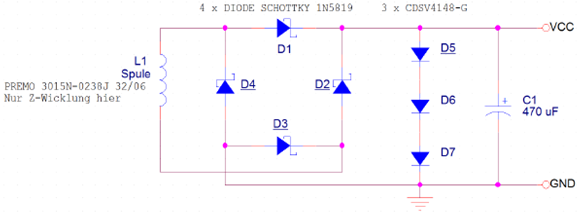
\includegraphics[width=0.5\textwidth]{3Vorgehen/imag/Schema_Harvester_PA.png}
    \caption{Harvesterschaltung der PA15(\cite{PA_bicycle})}
    \label{schema_harvester_pa15} 
\end{figure}

Die Harvesterschaltung der Abbildung \ref{schema_harvester_pa15} wurde im Rahmen der Machbarkeitsstudie erarbeitet. Die Schaltung besteht aus wenigen Teilen, die Spannungbegrenzung wurde mit drei Dioden in Durchlassrichtung realisiert, hier gibt es wahrscheinlich bessere Möglichkeiten die Spannung zu begrenzen, ohne Leistung zu verschwenden.

\subsubsection{EM8500-Chip}

Das EM-Evaluationsboard soll ebenfalls auf der neuen Leiterplatte Platz finden, das Schema inklusive aller Kondensatoren ist im Datenblatt zu finden. Jedoch wurden die Jumper nicht übernommen und nur einige Stecker wurden übernommen, bzw. mit eigenen Signalen ergänzt (siehe Abbildung \ref{schema_em-chip_inkl_peripherie}).


\begin{figure}[ht]
    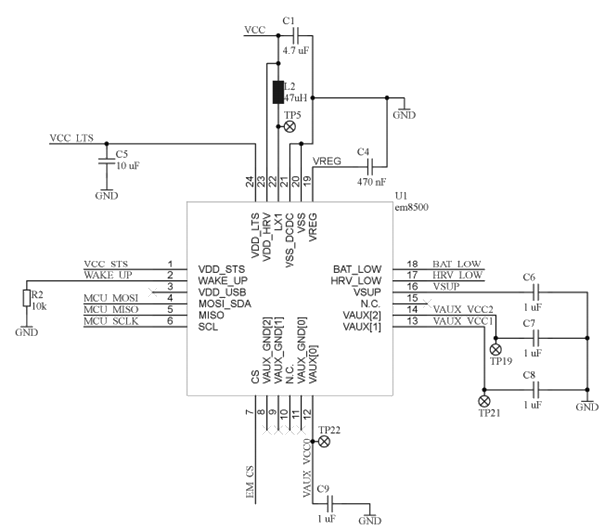
\includegraphics[width=1.0\textwidth]{3Vorgehen/imag/Schema_EM-Chip_inkl_Peripherie.png}
    \caption{Schema des EM-Chips mit der benötigten Peripherie}\label{schema_em-chip_inkl_peripherie} 
\end{figure}

\clearpage
\subsubsection{Energiespeicher}

Die Energiespeicher waren zum Zeitpunkt der Entwicklung der Hardware noch nicht definiert. Als Platzhalter wurden zwei Elektrolytkondensatoren (ElKo) mit den Werten aus der Machbarkeitsstudie eingefügt (siehe Abbildung \ref{schema_energiespeicher}). 

\begin{figure}[ht]
    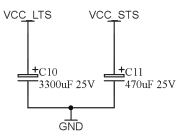
\includegraphics[width=0.3\textwidth]{3Vorgehen/imag/Schema_Energiespeicher.png}
    \caption{Schema der Energiespeicher (ElKos sind nur Platzhalter)}
    \label{schema_energiespeicher} 
\end{figure}


\subsubsection{Umlauferfassung}

Die Umlauferfassung kann nicht mit der verwendeten Spule realisiert werden, da bei der Energiegewinnung mit der Spule, das Signal gleichgerichtet wird. Die nicht benutzten Wicklungen der X- und Y-Wicklung liefern kein verwertbares Signal, was bereits in der Machbarkeitsstudie bewiesen wurde. Aus diesem Grund wird der Magnetdurchlauf mit einem Reed Switch detektiert und an das TI-SensorTag weitergegeben (siehe Abbildung \ref{schema_umlaufdetektion}). Ein Magnetdurchlauf erzeugt einen positiven Puls, solange sich der Magnet in der Reichweite des Reed Switch befindet.

\begin{figure}[ht]
    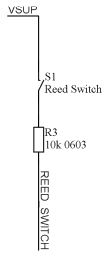
\includegraphics[width=0.1\textwidth]{3Vorgehen/imag/Schema_Umlaufdetektion.png}
    \caption{Schema Umlauferfassung}\label{schema_umlaufdetektion} 
\end{figure}

\subsection{Bauteildefinition und Optimierung}

Nachdem klar war, welche Teile auf der Leiterplatte Platz finden müssen, konnte die Optimierung der Schaltung in Angriff genommen werden. Ziel der Optimierung war es, bei 10 km/h genügend Energie zu gewinnen, damit das TI-SensorTag damit versorgt werden könnte. Dafür musste vor allem die Harvesterschaltung optimiert werden, damit keine Energie verloren geht. 
Es wurden folgende Punkte angeschaut und versucht zu optimieren:

\begin{enumerate}
    \item die Spule
    \item der Gleichrichter
    \item der Limiter
\end{enumerate}

\subsubsection{Die Spule}

Die Spule gewinnt die Energie aus dem an einer Speiche des Fahrrads befestigten Magneten. Eine stärkere Spule könnte mehr Energie aus dem vorbei schnellenden Magneten gewinnen. Entscheidend ist das die Fläche der Spule nicht vergrössert werden darf, bestenfalls sollte eine kleinere Spule gefunden werden, welche mehr Energie gewinnt. Gemäss der Formel 2.4 ist für die gewonnene Energie vor allem die Wicklungszahl entscheidend, jedoch wird bei den Spulen meistens nur die Induktivität angegeben. Die Induktivität hängt quadratisch von der Wicklungszahl und linear von der Fläche (siehe Formel \cite{equ_inductivity}) ab.

\begin{equation}
	L = \mu_0 \times \frac{N^2\times A}{l}
\end{equation}

Es wurde nach einer Spule mit einer höheren Induktivität und der gleichen Fläche gesucht, somit können nur noch zwei Variablen sich verändern. Zum einen kann sich die Wicklungszahl verändern und zum andern kann sich die Länge der Spule verändern. Die Spule von Würth Elektronik mit der Bezeichnung 74458308 hat eine ähnliche Fläche und eine grössere Induktivität, was auf den ersten Blick sehr vielversprechend aussieht.

Die Messung der erzeugten Spannung über der Spule hat ergeben, dass die Spule von Premo mit der Bezeichnung 3015N 0238J 3206, welche bisher verwendet wurde, eine höhere Spannung erzeugt als die neue Spule von Würth. Die Spule von Premo hat bei den Geschwindigkeiten von 10 km/h und 20 km/h eine grössere induzierte Spannung. Die Spule von Würth hat eine höhere Spannung bei den Geschwindigkeiten von 15 km/h und 40 km/h. Jedoch sollte die Schaltung für 10 km/h optimiert werden, somit wird der Spule von Premo der Vortritt gewährt. Nachfolgend wird der Unterschied zwischen den induzierten Spannungen in den Spulen ersichtlich (siehe Abbildungen \ref{messung_optimierung_spule} und \ref{blublu}). Der Unterschied ist nicht gross, jedoch muss hier die Spule von Premo bevorzugt werden, da die induzierte Spannung grösser ist.

\begin{figure}[ht]
 \begin{minipage}[t]{0.5\textwidth}
    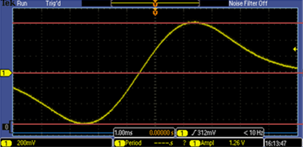
\includegraphics[width=0.9\textwidth]{3Vorgehen/imag/Messung_Optimierung_Spule_links.png}
    \caption{Spule von Premo}               
    \label{messung_optimierung_spule} 
 \end{minipage}
 \begin{minipage}[t]{0.5\textwidth}
    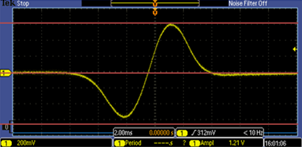
\includegraphics[width=0.9\textwidth]{3Vorgehen/imag/Messung_Optimierung_Spule_rechts.png}
    \caption{Spule von Würth}  
    \label{blublu}             
 \end{minipage}
\end{figure}

\subsubsection{Der Gleichrichter}

Der Gleichrichter aus der Machbarkeitsstudie bestand aus vier Dioden vom Typ 1N5819. Diese Dioden sind nicht für die Low-Power-Anwendung ausgelegt, ausserdem sind die Dioden nicht in einem Gehäuse verbaut. Wichtig ist bei dem Gleichrichter, dass die Leckströme möglichst klein sind und die Schwellenspannung sollte ebenfalls möglichst klein sein, damit wenig Energie verbraucht wird.

Es wurde als erstes eine Low-Power-Diode, mit der Bezeichnung HSMS-286P, getestet. Die Erwartungen waren entsprechend hoch, da diese Dioden für Low-Power-Anwendungen spezialisiert sind. Die Spule von Premo wurde als Quelle verwendet, um zu sehen, wie die Spannung nach dem Gleichrichter aussieht. Die Spannung nach dem Gleichrichter bestehend aus den Dioden vom Typ 1N5819 ist bei allen getesteten Geschwindigkeiten, also 10 km/h, 15 km/h, 20 km/h und 40 km/h, höher als beim Gleichrichter bestehend aus den Dioden vom Typ HSMS-286P. Der Spannungsunterschied liegt im Minimum bei ca. 40 mV. Der grösste Unterschied ist bei der Geschwindigkeit von 15 km/h ersichtlich, was in den Abbildungen \ref{messung_optimierung_gleichrichter_1} und \ref{pling} gezeigt wird.

\begin{figure}[ht]
 \begin{minipage}[t]{0.5\textwidth}
    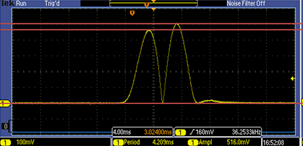
\includegraphics[width=0.9\textwidth]{3Vorgehen/imag/Messung_Optimierung_Gleichrichter_1_links.png}
    \caption{Gleichrichter 1N5819}
    \label{messung_optimierung_gleichrichter_1} 
 \end{minipage}
 \begin{minipage}[t]{0.5\textwidth}
    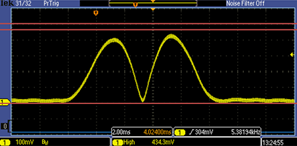
\includegraphics[width=0.9\textwidth]{3Vorgehen/imag/Messung_Optimierung_Gleichrichter_1_rechts.png}
    \caption{Gleichrichter HSMS-286P}
    \label{pling}
 \end{minipage}
\end{figure}

Als nächstes wurde ein Gleichrichter aus den Dioden vom Typ BAT54 getestet. Die Spannung nach dem Gleichrichter bestehend aus 1N5819 Dioden ist bei den Geschwindigkeiten von 15 km/h, 20 km/h und 40 km/h höher als nach dem Gleichrichter bestehend aus BAT54 Dioden. Der Spannungsunterschied liegt bei ca. 100 mVpp. Der Unterschied ist marginal, jedoch muss hier der Gleichrichter aus 1N5819 Dioden bevorzugt werden. Nur bei einer Geschwindigkeit von 10 km/h ist der Gleichrichter bestehend aus BAT54 Dioden besser als der Gleichrichter bestehend aus 1N5919 Dioden. Der Spannungsunterschied liegt hier bei ca. 10 mVpp. Dieser Unterschied ist vernachlässigbar, in Angesicht dessen, dass der Gleichrichter bestehend aus 1N5819 Dioden in allen anderen getesteten Geschwindigkeiten besser ist.

\begin{figure}[ht]
 \begin{minipage}[t]{0.5\textwidth}
    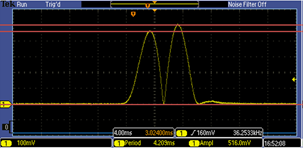
\includegraphics[width=0.9\textwidth]{3Vorgehen/imag/Messung_Optimierung_Gleichrichter_2_links.png}
    \caption{Gleichrichter 1N5819}
    \label{messung_optimierung_gleichrichter_2} 
 \end{minipage}
 \begin{minipage}[t]{0.5\textwidth}
    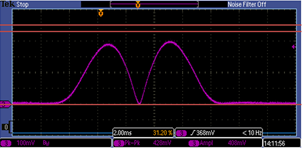
\includegraphics[width=0.9\textwidth]{3Vorgehen/imag/Messung_Optimierung_Gleichrichter_2_rechts.png}
    \caption{Gleichrichter BAT54}
 \end{minipage}
\end{figure}

\subsubsection{Der Limiter}

Die Spannungsbegrenzung, nachfolgend der Limiter genannt, ist ein sehr krititscher Teil der Harvesterschaltung, da die Spannung am EM-Chip Eingang nicht höher als 2 V sein darf, da ansonsten der EM-Chip beschädigt werden kann. Trotzdem soll möglichst wenig Energie verloren gehen, wenn die Spannungsbegrenzungsschaltung ihre Arbeit verrichtet. Bisher wurden drei Dioden in Durchlassrichtung in Serie geschaltet, um die Spannung zu begrenzen.

Herr Erich Ruff hat eine Spannungsbegrenzungsschaltung entwickelt, welche er uns freundlicherweise zur Verfügung stellte. Diese Schaltung wurde mit dem Limiter verglichen, welcher aus drei Dioden bestand.

Die Spannung nach dem Dioden-Limiter ist bei 10 km/h, 15 km/h und 20 km/h höher, jedoch ist die Rippelspannung ebenfalls höher. Nur bei einer Geschwindigkeit von 40 km/h ist die Spannung nach dem Limiter von Herr Erich Ruff, nachfolgend FET-Limiter genannt, besser, sowohl bei Spannungslevel als auch bei der Rippelspannung. Die Abbildung \ref{messung_optimierung_limiter} zeigt, dass der Dioden-Limiter eine höhere Spannung liefert, jedoch ist die Rippelspannung ebenfalls höher.

\begin{figure}[ht]
 \begin{minipage}[t]{0.5\textwidth}
    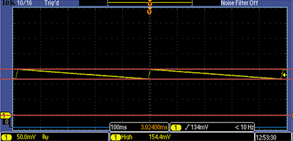
\includegraphics[width=0.9\textwidth]{3Vorgehen/imag/Messung_Optimierung_Limiter_links.png}
    \caption{Dioden-Limiter}
    \label{messung_optimierung_limiter} 
 \end{minipage}
 \begin{minipage}[t]{0.5\textwidth}
    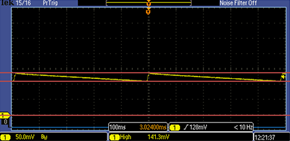
\includegraphics[width=0.9\textwidth]{3Vorgehen/imag/Messung_Optimierung_Limiter_rechts.png}
    \caption{FET-Limiter}
 \end{minipage}
\end{figure}

\subsection{Layout}

Schlussendlich musste aus den optimierten Teilen des Schemas eine Leiterplatte gestaltet werden. Die meisten Footprints waren bereits in den Bibliotheken des InES vorhanden, einige mussten neu gezeichnet werden.

\subsubsection{Positionierung}

Die Positionierung der einzelnen Teile kann sehr wichtig sein, da mit einer guten Positionierung bereits unnötige Leiterbahnverläufe verhindert werden können. Ebenfalls können gut positionierte Bauteile die Spannungspegel stabilisieren. Es wurde darauf geachtet, dass die Bauteile, welche zu einem Block gehören, nahe beieinander zu platzieren, um unnötig lange Signallaufwege zu verhindern.

Die Bauteile der Harvesterschaltung wurden als Block so nahe wie möglich beieinander platziert und wo immer möglich wurden die Speisungsleitungen mit einer Leiterbahnbreite von 20 Mil gezogen, damit der Widerstand der Leiterbahn (\cite{eqn_res_leiter}) möglichst klein gehalten wurde. Der Leiterwiderstand konnte so minimiert werden, was verhindert, dass die Energie in den Leiterbahnen verschwendet wird.

\begin{equation}
	R = \rho \times \frac{l}{A}
\end{equation}

Der Widerstand bei 10 Mil ist somit ca. 1.9 m$\Omega$ pro Meter, 
der Leiterwiderstand bei einer Leiterbahnbreite von 20 Mil ist ca. 1.0 m$\Omega$ pro Meter. Problematisch ist, dass sich der Block der Harvesterschaltung etwas entfernt vom Block des EM-Chips befindet. Das bedeutet, dass die Leiterbahn mit der Speisung des EM-Chips mehrere Zentimeter zurücklegen muss. Sicherlich ist der Unterschied im Widerstand nicht sehr gross, doch die Energie, welche in der Leiterbahn verloren gehen würde, konnte so halbiert werden.

Der wichtigste Aspekt der Platzierung des EM-Chips war, dass die Stützkondensatoren so nah wie möglich am EM-Chip platziert wurden, damit die Spannung am EM-Chip so konstant wie irgend möglich gehalten werden kann.

\begin{minipage}{1\textwidth}
Ein wichtiger Punkt ist die Platzierung des Steckers, welcher unsere Leiterplatte mit dem TI-SensorTag verbindet. Durch eine Falschplatzierung kann es hier passieren, dass die beiden Leiterplatten nicht korrekt übereinander ausgerichtet sind, wenn sie aufeinander gesteckt werden. Das ist eher ein ästhetisches Problem, jedoch kann das auch Probleme beim Einbauen in ein Gehäuse bereiten. Zu dem Stecker gehört auch die Platzierung der Testpunkte, welche direkt mit dem Stecker verbunden sind. Gemäss dem Wunsch der Betreuer wurde hier ein Rastermass von 2.5 mm der Testpunkte eingehalten, so dass eine Steckerleiste eingelötet werden könnte. Problematisch ist jedoch, dass die Testpunkte einen grossen Raum der Leiterplatte einnehmen, wie in Abbildung \ref{layout_testpunkteraster} ersichtlich.
\end{minipage}

\begin{figure}[ht]
    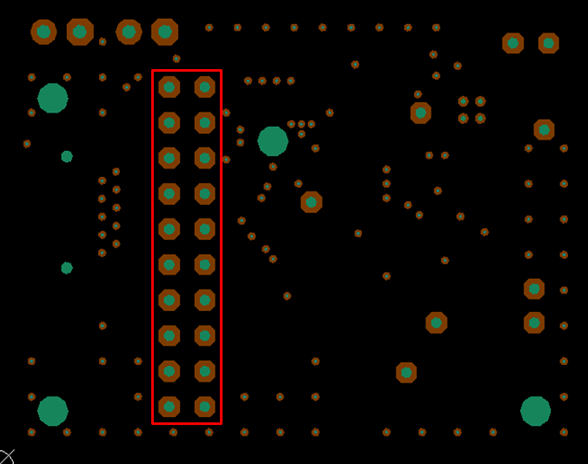
\includegraphics[width=0.8\textwidth]{3Vorgehen/imag/Layout_Testpunkteraster.png}
    \caption{Pads der Leiterplatte, rot eingerahmt die Testpunkte des Steckers}\label{layout_testpunkteraster} 
\end{figure}

\subsubsection{Das erste Layout}

Die erste Version der Leiterplatte war mit vielen Forderungen der Betreuer ausgestattet. Alle Netze wurden mit Testpunkten ausgestattet. Die Testpunkte des Steckers wurden im Rastermass 2.5 mm angeordnet und die Netze der Spannung nach dem Harvester, die Spannung des Short- und Long-Term-Storage wurden mit Strommesspunkten ausgestattet. Es wurden ebenfalls Montagelöcher platziert, jedoch sind diese sehr minimalistisch, da nur eine M2-Schraube durchpasst. Besser wäre es, Montagelöcher für M3-Schrauben zu platzieren, doch der Platz auf der Leiterplatte ist sehr limitiert. Die Leiterplatte ist nur 33 x 42 mm gross, was ein Milimeter breiter ist als das TI-SensorTag. Der Anschluss der Energiespeicher wurde so realisiert, dass die Energiespeicher nicht auf der Leiterplatte Platz finden, da der Platz nicht ausreicht.


\subsubsection{Das Redesign}

Das Layout wurde von Herr Olivier Rion begutachtet. Seine Kritikpunkte werden auf der nächsten Seite aufgelistet.

\newpage
\begin{minipage}{1\textwidth}

Kritikpunkte am Schema:
\begin{enumerate}
    \item VCC sollte in Pfeil sein: Das Symbol für VCC und generell alle Speisungen sollten als Pfeil im Schema dargestellt werden.
    \item Generell für eine erste Version sind viele TP gut.
    \item Auf dem Schema fehlt noch ein Symbol für die GND Pads für Messungen: Auf dem Top-Layer des Layouts wurde eine Fläche von Lötstopplack freigestellt, dies sollte auf dem Schema verzeichnet werden.
	\item Die freien Pins auf X1 sollten mit IO angeschlossen sein: Die nicht verwendeten Pins vom EM8500-Chips sollten mit dem Stecker X1 verbunden werden, jedoch ist das problematisch, da eine direkte Verbindung zum Mikroprozessor Energie verbrauchen kann, solange der Mikroprozessor nicht gestartet ist.
	\item Unten links auf dem Schema fehlt die Versionen, die Beschreibung, usw.
	\item Eine kleine Beschreibung beim Harvester wäre gut, z.B. Prinzip mit T1, Spannungsregulierung usw.: Eine Beschreibung hilft die Schaltung schneller zu verstehen, dass macht eine Übergabe an die nachfolgenden Studenten einfacher.
\end{enumerate}


Kritikpunkte am PCB:
\begin{enumerate}
    \item Die Grenze vom Print sollte mit Mechanical und keepOutLayer gemacht werden.
    \item Loch oben links: Die Leiterbahnen sind zu nah um die Löcher platziert, es sollte ein keepOutLayer um die Löcher platziert werden.
    \item Die Leiterbahnen sollten immer in Gruppen platziert werden.
	\item GND kann Kontakt mit den Schraubenköpfen haben: Es muss sichergestellt werden, dass die Schraube keinen Kontakt mit den Leitungen hat und dass die Flächen nicht unter dem Schraubenkopf platziert werden. 
\end{enumerate}

Wir sind dankbar für konstruktive Kritik, jedoch kann diese Kritik aus zeitlichen Gründen noch nicht umgesetzt werden. Neben den Kritikpunkten von Herr Rion wurden während der Arbeit noch weitere Kritikpunkte ersichtlich.

\begin{enumerate}
    \item Die Testpunkte auf der Leiterplatte müssen neu platziert werden, weil sie Teilweise auf der Unterseite nicht angelötet werden können, da die Spule sie verdeckt. 
    \item Die Abstände zwischen den Testpunkten müssen vergrössert werden, damit eine KO-Sonde gut daran befestigt werden kann ohne einen Kurzschluss zu verursachen.
    \item Der Footprint vom Stecker X1 muss überarbeitet werden, da dieser falsch erfasst wurde.
	\item Die Position des Steckers X1 muss verändert werden, da die Position nicht mit dem Gegenstück des TI-SensorTags übereinstimmt.
	\item Die Netze VCC\_STS, VCC\_LTS und VREG dürfen nicht mit dem Stecker X1 verbunden werden, da die Energie über diese Anschlüsse verloren geht.
\end{enumerate}
\end{minipage}

\newpage
Die Punkte 3 bis 5, welche den Stecker X1 betreffen konnten vor Abschluss noch überarbeitet werden, jedoch wäre die Lieferzeit für die Leiterplatte zu lang, als dass die Leiterplatten vor Abgabe der Arbeit eintreffen würden. Darum wurden alle Messungen mit der ersten Version der Leiterplatte durchgeführt.


% 4----------------------------------------------------------
\section{Inbetriebnahme des Prototypen}

Nach der Entwicklung der neuen Hardware musste diese getestet werden, um die Funktionsweise mit den bisherigen Messungen zu verifizieren. Es werden generell zwei wichtige Messstellen (siehe Abbildung \ref{EnergieMessungStellen}) ersichtlich. Die erste befindet sich nach dem Harvester und vor dem EM8500-Chip, die zweite wichtige Messstelle befindet sich zwischen dem EM8500-Chip und dem TI-SensorTag. Es ist wichtig die Leistungs- oder Energiemessung durchzuführen, da diese Werte essentiell für die Einstellung des EM8500-Chips und die Entwicklung der Firmware für das TI-SensorTags sind. 

\begin{figure}[ht]
  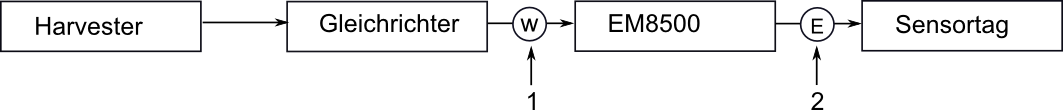
\includegraphics[width=1.0\textwidth]{3Vorgehen/imag/EnergiemessungStellen.png}               
  \caption{Messstellen am Prototypen}
  \label{EnergieMessungStellen} 
\end{figure}

\subsection{Testen der Harvesterschaltung}
\label{glace}

\subsubsection{Leistungsverifizierung}
\label{leistungsverifizierung}

Es wurde eine Leistungskennline der Harvesterschaltung aufgenommen, um die verfügbare Leistung zu verifizieren. Wichtig ist, dass die verfügbare Leistung im gleichen Bereich ist, wie beim fliegenden Aufbau. 

\begin{minipage}{1\textwidth}
\captionof{table}{Leistung des fliegenden Aufbaus}
\label{tab:leistung_fliegenden-aufbaus} 
\begin{tabbing}
    Geschwindigkeit   \quad\= maximale Leistung    \quad\= MPP-Ratio\\[0.8ex]
    10 km/h        \> 12.87 $\mu$W  \> 43.23 \%\\
	20 km/h        \> 43.35 $\mu$W  \> 45.51 \%\\
	40 km/h        \> 250.26 $\mu$W  \> 48.44 \%
\end{tabbing}
\end{minipage}

\begin{minipage}{1\textwidth}
\captionof{table}{Leistung der neuen Leiterplatte}
\label{tab:leistung_neuen_leiterplatte} 
\begin{tabbing}
    Geschwindigkeit   \quad\= maximale Leistung    \quad\= MPP-Ratio\\[0.8ex]
    10 km/h        \> 10.17 $\mu$W  \> 56.99 \%\\
	20 km/h        \> 48.57 $\mu$W  \> 61.82 \%
\end{tabbing}
\end{minipage}

Die maximal zur Verfügung stehende Leistung wurde etwas kleiner, bei dem fliegenden Aufbau betrug die maximale Leistung bei 10 km/h ca. 12 $\mu$W, die maximale Leistung bei der neuen Leiterplatte beträgt ca. 10 $\mu$W. Jedoch ist bei einer Geschwindigkeit von 20 km/h die Leistung der neuen Leiterplatte besser und der MPP wurde ebenfalls verschoben, was ein grosser Vorteil ist, da die Einstellung des MPPT-Ratio auf dem EM8500-Chip konfiguriert werden kann. Bisher konnte das MPPT-Ratio nicht korrekt auf die Hardware eingestellt werden, da die Einstellung nur Werte zwischen 50\thinspace\% und 80\thinspace\% akzeptiert.

\subsubsection{Testen der Spule}\label{starkeSpule}

Es wurde klar, dass die Energie, welche die Harvesterschaltung mit der aktuellen Spule von Premo mit einer Induktivität von 2.38 mH liefert zu klein ist und verbessert werden muss. Ideen wurden gesammelt und Herr Marcel Meli bemerkte, dass noch eine Spule von Premo mit einer Induktivität von 4.77 mH vorhanden wäre, diese sollte getestet werden. Die Spule hatte den exakt gleichen Aufbau wie die Spule, welche bis anhin verwendet wurde, nur die Induktivität war höher. Gemäss der Formel \cite{equ_inductivity} ist die Induktivität von der Wicklungszahl abhängig. Die Wicklungszahl wiederum beeinflusst die induzierte Spannung.

\captionof{table}{Leistung mit unterschiedlichen Spulen}
\begin{tabbing}
    Spule\hspace{2cm}   \quad\= maximale Leistung    \\[0.8ex]
    Premo 2.38 mH        \> 48.57 $\mu$W\\
	Premo 4.77 mH        \> 66.82 $\mu$W\\
	
\end{tabbing}

Die Messung hat ergeben, dass die Energie bei einer Verdoppelung der Induktivität eine Leistungssteigerung von ca. 37\thinspace\% zur Folge hat. Dies lässt sich auch mathematisch nachweisen:

\begin{flalign}
	&L = \mu_0 \times \frac{N^2\times A}{l}\\
	&N = \sqrt{\frac{L\times l}{\mu_0\times A}}\\
	&neue\,Wicklungszahl = \sqrt{2} \times bisherige\,Wicklungszahl
\end{flalign}

Da die Leistung von der induzierten Spannung abhängt und die induzierte Spannung von der Wicklungszahl abhängt, steigt die Leistung in Abhängigkeit zur Wicklungszahl. Ein Zuwachs der Leistung von bis zu 41\thinspace\% war zu erwarten. Es wurde entschieden, dass die stärkere Spule mit einer Induktivität von 4.77 mH verwendet werden soll.

\subsubsection{Testen Magnete in Serie}

Herr Dario Dündar machte uns auf ein Produkt von Reelight aufmerksam. Die Firma Reelight stellt Lichter für das Fahrrad her welche über Energy Harvesting betrieben werden, dafür werden neben der Wirbelstromvariante (siehe Unterkapitel Ausgangslage \ref{ausgang}) ebenfalls Produkte mit speziellen Magneten verwendet. Leider war kein Datenblatt für die Magnete mit der Bezeichnung RE-10200 vorhanden und auch auf Nachfrage wurde kein Datenblatt oder Ähnliches herausgegeben. Jedoch konnte man herausfinden, dass in dem Gehäuse drei Magnete verbaut sind, welche stärker sind als unsere Magnete. Unsere Magnete haben eine N42 Magnetisierung, was bedeutet, dass sie eine Remanenz von 1.29 – 1.32 Tesla haben. Die Magnete, welche im Gehäuse von Reelight verbaut sind, haben eine N45 Magnetisierung, was bedeutet sie haben eine Remanenz von 1.37 – 1.42 Tesla. Der Durchmesser der Magnete beträgt 2.5 mm. Unsere bisher verwendeten Magnete wiesen einen Durchmesser von 20 mm auf. 

Es wurde eine Leistungskennlinie mit dem Magneten von Reelight aufgenommen. Die maximale zur Verfügung stehende Leistung betrug 135.50 $\mu$W, was einem Zuwachs von über 100\thinspace\% entsprach.

\captionof{table}{Leistung mit unterschiedlicher Anzahl an Magneten}
\begin{tabbing}
    Konfiguration\hphantom{4.77 mH, 3 Magnete in Serie (Reelight)}   \quad\= maximale Leistung    \\[0.8ex]
    Spule Premo 4.77 mH, 1 Magnet in Serie        \> 66.82 $\mu$W\\
	Spule Premo 4.77 mH, 3 Magnete in Serie (Reelight)        \> 135.50 $\mu$W
\end{tabbing}

Diese Messung brachte uns auf die Idee einen weiteren Versuch zu realisieren. Wir modifizierten den Testaufbau, damit zwei Magnete direkt hintereinander montiert werden konnten. Es sollte untersucht werden, ob die beiden Magnete die Spule besser anregten als nur ein Magnet. Die induzierten Spannungswerte unterschieden sich nicht drastisch, jedoch wurde die Spule länger angeregt. Die Abbildungen \ref{zweiMagneteInSerie} und \ref{manu} zeigen den Unterschied zwischen einer Spule, welche nur von einem Magneten angeregt wurde und einer Spule, welche von zwei direkt aufeinander folgenden Magneten angeregt wurde. Es ist zu sehen, dass die Spannung in der Spule, welche nur mit einem Magneten angeregt wurde, höher ist, jedoch wesentlich kürzer anliegt. Es wurde, trotz dem Potential für mehr Energie mit zwei Magneten, dagegen entschieden zwei Magnete in Serie einzusetzen, da man dieses Prinzip wieder ins Extreme treiben könnte und das ganze Rad mit Magneten ausstatten könnte. Sicherlich würde das jegliches Energieproblem unserer Arbeit lösen, jedoch wäre dies unpraktisch, wegen der verstärkten Bremswirkung und es wäre unästhetisch.

\begin{figure}[ht]
 \begin{minipage}[t]{0.5\textwidth}
  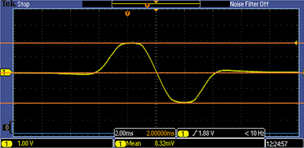
\includegraphics[width=0.9\textwidth]{3Vorgehen/imag/zweiMagneteInSerie_links.png}
  \caption{Anregung der Spule mit einem Magneten}
  \label{zweiMagneteInSerie} 
 \end{minipage}
 \begin{minipage}[t]{0.5\textwidth}
  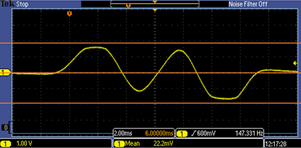
\includegraphics[width=0.9\textwidth]{3Vorgehen/imag/zweiMagneteInSerie_rechts.png}
  \caption{Anregung der Spule mit zwei Magneten in Serie}
  \label{manu}
 \end{minipage}
\end{figure}


\subsection{Ausmessen der Leistung der endgültigen Hardware}

Gemäss dem vorangegangen Unterkapitel \ref{glace} Abschnitt \ref{starkeSpule} wurde ersichtlich, dass die stärkere Spule verwendet werden sollte. Wir haben uns jedoch gegen die Variante mit zwei Magneten in Serie entschieden, trotzdem könnte dies später verwendet werden. Es musste erneut die Leistung, welche die Harvesterschaltung zur Verfügung stellt, aufgenommen werden.

\todo{xxxxxxxxxxxxxxxxxxxxxxxxxxxxxxxxxxxxxxxxxxxxxxxxxxxxxxxxxx}

\begin{minipage}{\textwidth}
\captionof{table}{Leistung des Prototypen}
\begin{tabbing}
    Geschwindigkeit   	\quad\= maximale Leistung    \\[0.8ex]
    10 km/h		        \> 24.77 $\mu$W\\
	15 km/h		        \> 61.07 $\mu$W\\
	20 km/h		        \> 116.69 $\mu$W\\
	40 km/h		        \> 472.61 $\mu$W\\
\end{tabbing}
\end{minipage}

Die maximal verfügbare Leistung konnte durch die stärkere Spule erneut deutlich verbessert werden. 

\subsection{Ausmessen der Energieabgabe EM8500-Chip}
\label{em_enerige_ausgang}

Es war nun bekannt, wie viel Leistung die Harvesterschaltung zur Verfügung stellte, jedoch musste die Leistungsabgabe nach dem konfigurierten EM8500-Chip noch erfasst werden. Diese Angabe war sehr wichtig, um die Entwicklung der Firmware zu optimieren. Diese Werte gaben einen Rahmen, wie viel Energie das TI-SensorTag verbrauchen durfte.

Da es sich beim Ausgang des EM8500-Chips um eine Spannungsquelle handelt, welche bei uns auf 2 V konfiguriert wurde, konnte man die Energie, welche zur Verfügung stand, messen. Der Ausgang des EM8500-Chips wurde für diesen Zweck mit einem 10 k$\Omega$ Widerstand belastet. Anschliessend wurde gemessen, wie lange die Spannung am Ausgang aufrecherhalten werden konnte. Die Abbildung \ref{EnergieEMChip15kmh} zeigt den Spannungsverlauf über der Last. Da der Spannungsverlauf annähernd ein Rechteck war, konnte die Energie anhand der Zeit, welche der Ausgang aktiv war, berechnet werden.

\begin{equation}
	E = \frac{U^2}{R}  \times \Delta t
\end{equation}

\begin{figure}[ht]
  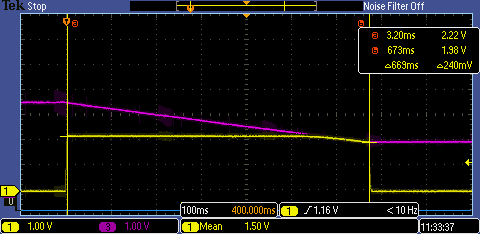
\includegraphics[width=0.80\textwidth]{3Vorgehen/imag/EnergieEMChip15kmh.PNG}
  \label{EnergieEMChip15kmh} 
  \caption{rot: VCC\_STS, gelb: VSUP}
\end{figure}



\captionof{table}{Leistungsabgabe Ausgang EM8500}
\label{tab:em_out_zsm}
\begin{tabbing}
    Geschwindigkeit   	\quad\= abgegebene Energie    \\[0.8ex]
    10 km/h		        \> 261.2 $\mu$Ws\\
	15 km/h		        \> 267.6 $\mu$Ws\\
	20 km/h		        \> 273.2 $\mu$Ws\\
	40 km/h		        \> 373.2 $\mu$Ws\\
\end{tabbing}

% 5---------------------------------------------------------------------------
\section{Energy Management}

Das Ziel des Energy Managements ist es, dass die zur Verfügung stehende Energie bei 10 km/h genügt, um BLE-Pakete zu versenden. Die sekundäre Aufgabe ist es, dass sich der LTS lädt und entlädt. Ein Laden des LTS ohne dass die Energie im LTS verwertet werden kann ist Energieverschwendung. Die zwei gestellten Aufgaben sollen durch möglichst optimale Speichergrössen und intelligente Schwellwerte erreicht werden.

Damit man die Kondensatorenwerte berechnen kann, braucht es Energiedaten. Deshalb stehen als erstes im Unterkapitel \ref{v_messungen_sensortag} die Energie-Messergebnisse, danach folgt im zweiten Unterkapitel \ref{v_e_kalkulation} die Dimensionierung der Kondensatoren und dann das Berechnen der Schwellwerte in Unterkapitel \ref{v_schwellwerte}. Als letzer Punkt werden die Energiezustände innerhalb des Bicycle Computers definiert. Dies, weil die letzte offene Aufgabe der Optimierungsliste (\ref{optimierung}) das Senden nach 10 s dem Energiezustand angepasst werden soll.


% x.1 ------------------------
\subsection{Energiemessungen}
\label{v_messungen_sensortag}


Die Entwicklung ist konstant begleitet durch Energiemessungen. Sei dies durch Leistungsmessungen bei der Hardware (Harvester und EM8500-Chip) oder sei dies als Energiemessung der Software (TI-SensorTag). Für die Energiemessungen wird der Power Analyser von Agilent Electronic N6705B verwendet. Dieses Messgerät misst gleichzeitig Strom, Spannung und Leistung im Zeitverlauf. Annäherungen aus den Messungen mit einem Oszilloskop sind nicht mehr notwendig.

In diesem Unterkapitel werden die Resultate den TI-SensorTag-Energiemessungen dargestellt. Mehr Messgrafiken und Erklärungen sind im Messprotokoll (\cite{messung_energie_sensortag}) abgelegt. Den Überblick über die Versionen ist in der untenstehenden Tabelle aufgelistet. 


\subsubsection{Überblick Energiemessungen}\label{erst_EMessungen}

\begin{figure}[ht]
    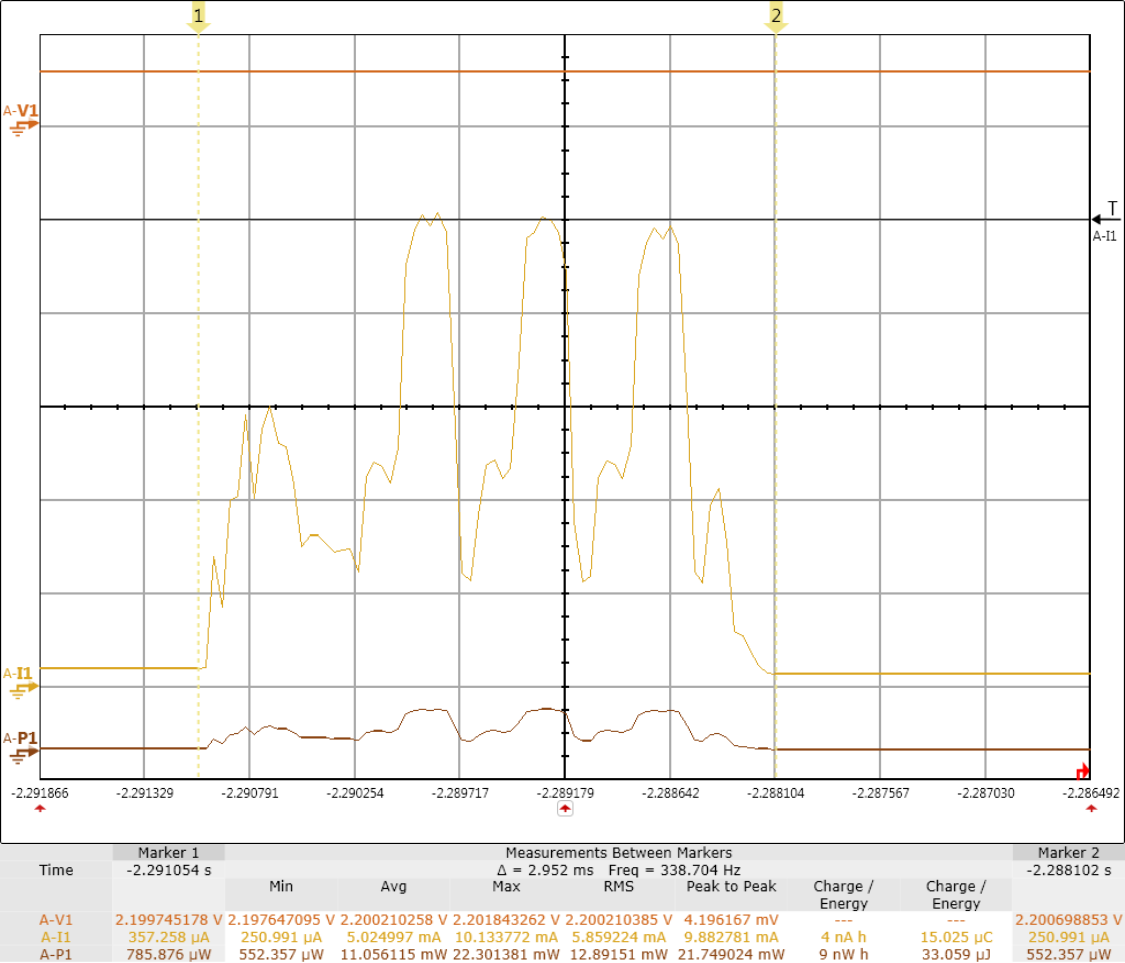
\includegraphics[width=1.0\textwidth]{3Vorgehen/imag/v0Send33uJ.png} 
    \caption{Minimalster Energieverbrauch: 3 BLE Pakte über Advertising Mode senden}
    \label{BLE_send}
\end{figure}

Um einen ersten Anhaltspunkt über den Energieverbrauch des TI-SensorTags zu erhalten, werden drei BLE-Pakete im Advertsing Mode per Knopfdruck gesendet (siehe Abbildung \ref{BLE_send}). Dies entspricht der Messung zur TI-SensorTag-Version V0. Nach der Weiterentwicklung des Programms zum Auslesen der Sensoren, folgte die Messung der Version V1. In dieser Version wird die GPIO ausgelesen. Die GPIO ist für das Einlesen der Reed Switch-Impulse unumgänglich. Die Version V2, der Versuch mehr Sleep-Time einzubauen, scheitert am Zusammenspiel des Timings der BLE-Radio-Interrupts mit den GPIO-Interrupts. Durch das Neuaufsetzen des Programms entsteht die Version V3. Diese sendet power-optimiert Geschwindigkeitspakete. 

Die untenstehende Tabelle stellt die Energieresultate dar. Unterschieden wird zwischen dem Energieverbrauch für die Initialisierung, kurz Init, und der Energie zum Senden von drei BLE-Paketen. Die Diskussion über Energieoptimierungen und die Deutung der Resultate finden sich in den Sitzungsprotokollen vom \cite{sitzungsprotokoll_160226} - \cite{sitzungsprotokoll_160516_ms3}.

\begin{minipage}{\textwidth}
\captionof{table}{Messresultate nach TI-SensorTag-Versionen}
\begin{tabbing}
    Version   \quad\= Datum    \quad\= Aufgabe\hphantom{re, kein Schlafmodus optimiert} \quad\= Energie Init    \quad\=  Energie Senden \\[0.8ex]
    V0        \> 10.3.16  \> Nur BLE Paket      \> unbekannt            \> 33 $\mu$J \\
    V1        \> 16.3.16  \> mit Geschwindigkeit      \> 87 $\mu$J            \> 32 $\mu$J \\
    V3        \> 22.4.16   \> Schlafmodus optimiert     \> 40 $\mu$J            \> 29 $\mu$J \\
    V4        \> 03.6.16    \> 3 Sensore, kein Schlafmodus optimiert     \> 77 $\mu$J            \> 43 $\mu$J \\
    V5        \> ongoing    \> 3 Sensore mit optimiertem Schlafmodus     \> unbekannt           \> unbekannt\\
\end{tabbing}
\end{minipage}

Bei den ersten drei Messungen werden die Sensoren noch nicht ausgelesen. Es zeigt sich, dass das Auslesen der Sensoren über I2C und das Warten, bis die Sensoren gestartet sind,  mehr Energie verbraucht als erwartet. Der Energieverbrauch für das Auslesens eines Sensors ist ohne Optimierungsmassnahmen so gross, dass kein Senden der Daten möglich ist. Die Speisung der Applikation bricht zusammen (siehe Abbildung \ref{i2c_problem}).

\begin{figure}[ht]
    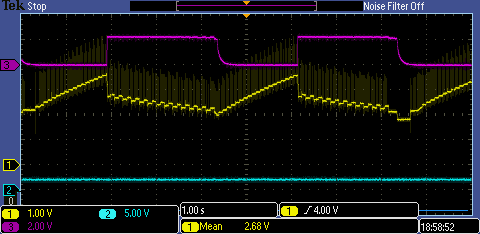
\includegraphics[width=0.5\textwidth]{3Vorgehen/imag/pic4VSUPbrichtEin.PNG} 
    \caption{Auslesen der Sensoren verursacht Einbrechen der Energie}
    \label{i2c_problem}
\end{figure}

Aus diesen Grund wurde die Poweroptimierung innerhalb des Programms zur zentralen Herausforderung in dieser Arbeit. Details darüber sind im nächsten Unterkapitel (\ref{powerOptimierung} Power Management) zusammengefasst. Bei der Version V4 zeigt sich, dass die Funktion BLE-Send, zu der auch das Einlesen der Sensordaten gehört, einen Zuwachs von 50\thinspace\% an Energiebedarf bewirkt. 



\subsubsection{Resultate Energieverbrauch TI-SensorTag Applikation V4}
\label{energie_sensortag} 

Als Überblick über den konkreten Energieverbrauch bei der Version V4 (siehe Messprotokoll \cite{messung_energie_sensortag}) folgt exemplarisch ein Bild zur Initialisierung (Abbildung \ref{energie_init}), eines zum Senden der drei BLE-Pakete (Abbildung \ref{energie_senden}) und dann je eine Abbildung zum Energieverbrauch beim Starten der drei Sensoren. Die Abbildung \ref{energie_ueberblick} zeigt den Überblick eines erstmaligen Sendens. Ganz links ist das einmalige Aufladen der Kondensatoren auf dem TI-SensorTag zu sehen. Dieser Vorgang ist in Abbildung \ref{energie_kondensatoren_sensortag} vergrössert dargestellt. Aus der Abbildung \ref{energie_ueberblick}, die den Überblick des Sendens darstellt, kann man die durchschnittliche Zeit, nach der ein Refresh erfolgt ungefähr herauslesen. Durchschnittlich folgt ca. alle 0.1 s ein Refresh-Peak. Auch dieser Vorgang ist als einzelne Energiemessung aufgenommen und in Abbildung \ref{Energieverbrauch senden eines BLE-Paketes mit Sensordaten} dokumentiert. Am Schluss dieses Unterkapitels werden alle Energiewerte in einer Tabelle zusammengefasst.

\clearpage

\begin{figure}[p]
  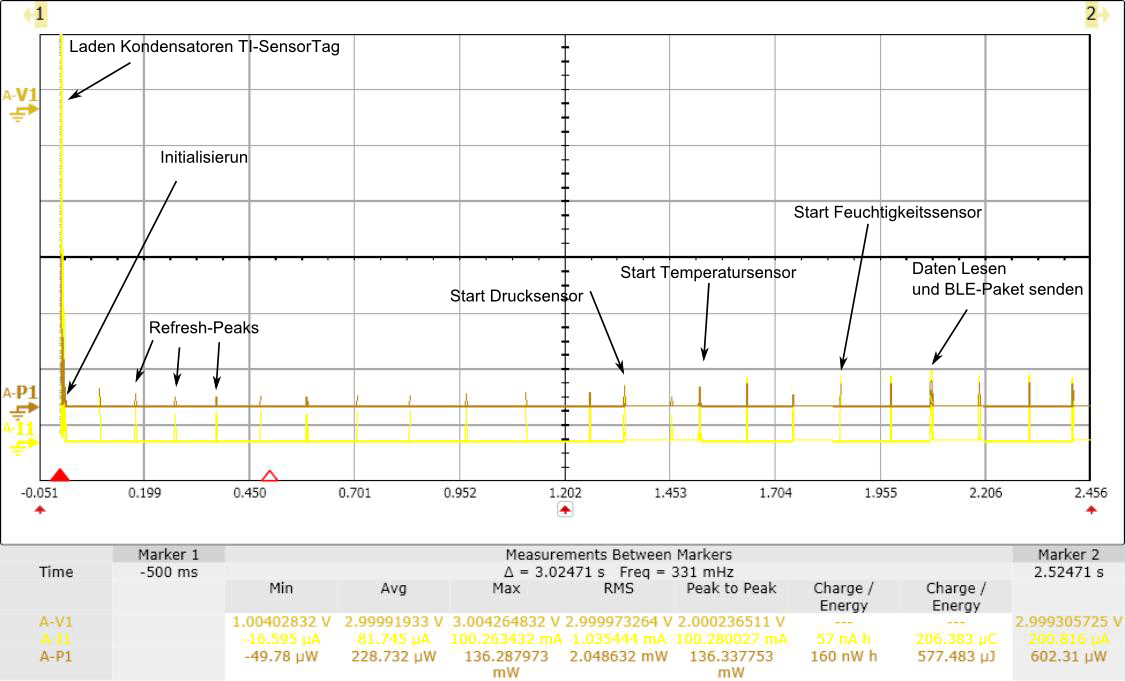
\includegraphics[width=1.0\textwidth]{3Vorgehen/imag/Ueberblick.png}
  \caption{Überblick Energieverbrauch mit Refreshzyklen}
  \label{energie_ueberblick}
 
  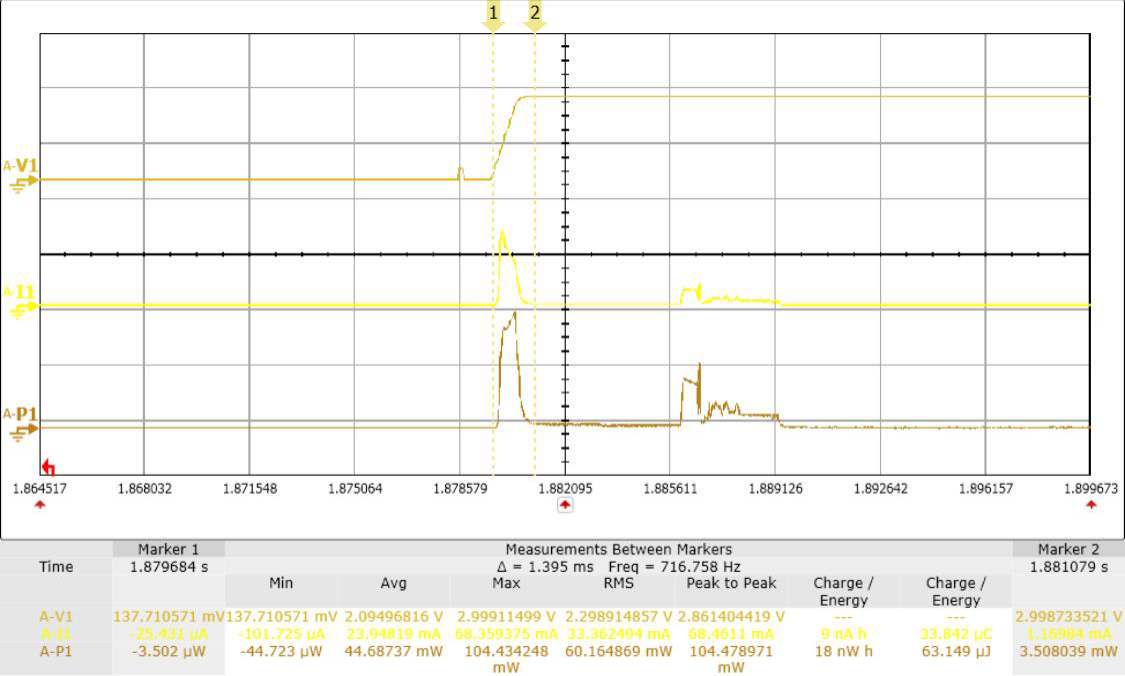
\includegraphics[width=1.0\textwidth]{3Vorgehen/imag/Energie_Laden_Kondensatoren_Sensortag.png}
  \caption{Einmaliges Aufladen der Kondensatoren TI-SensorTag}
  \label{energie_kondensatoren_sensortag}
\end{figure}

\clearpage

\begin{figure}[p]
  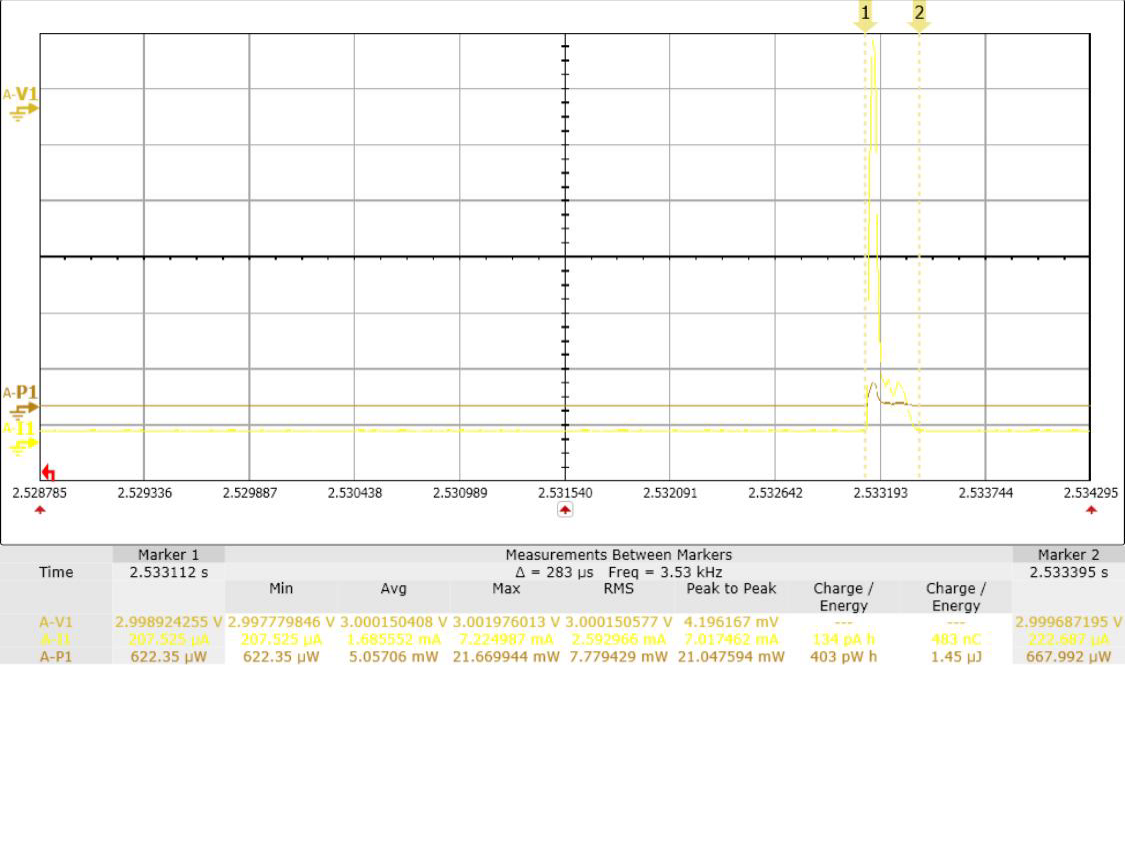
\includegraphics[width=1.0\textwidth]{3Vorgehen/imag/Refresh.png}
  \caption{Energieverbrauch Refreshzyklus}
  \label{energie_refresh}

  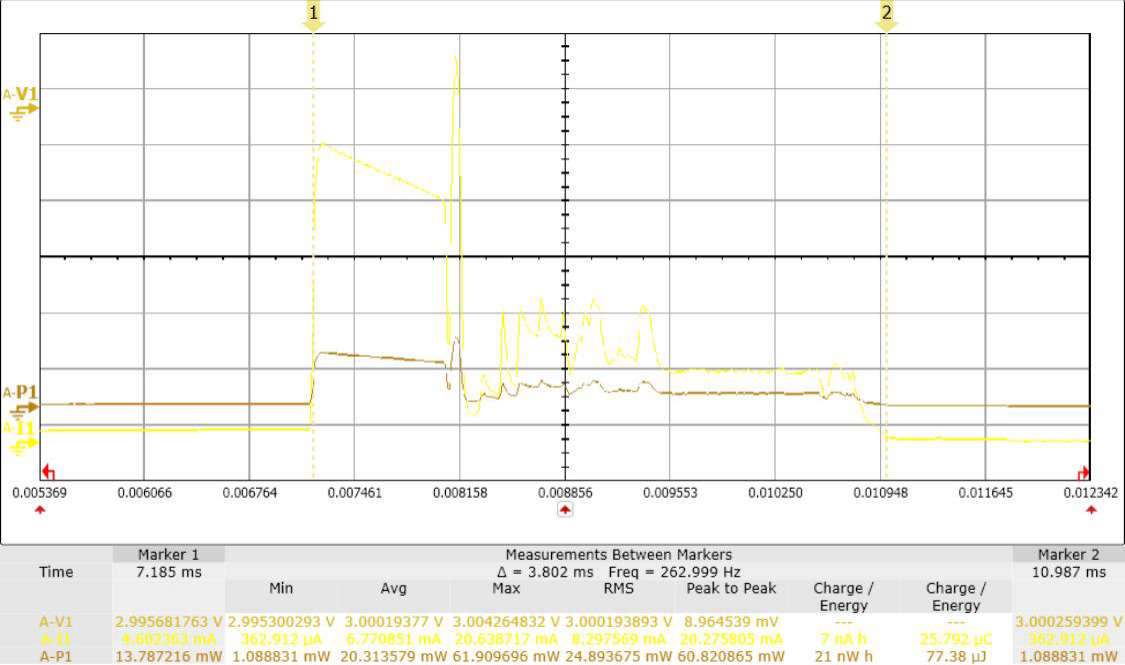
\includegraphics[width=1.0\textwidth]{3Vorgehen/imag/Init.png}
  \caption{Energieverbrauch für Initialisierung}
  \label{energie_init}
\end{figure}

\clearpage

\begin{figure}[p]
  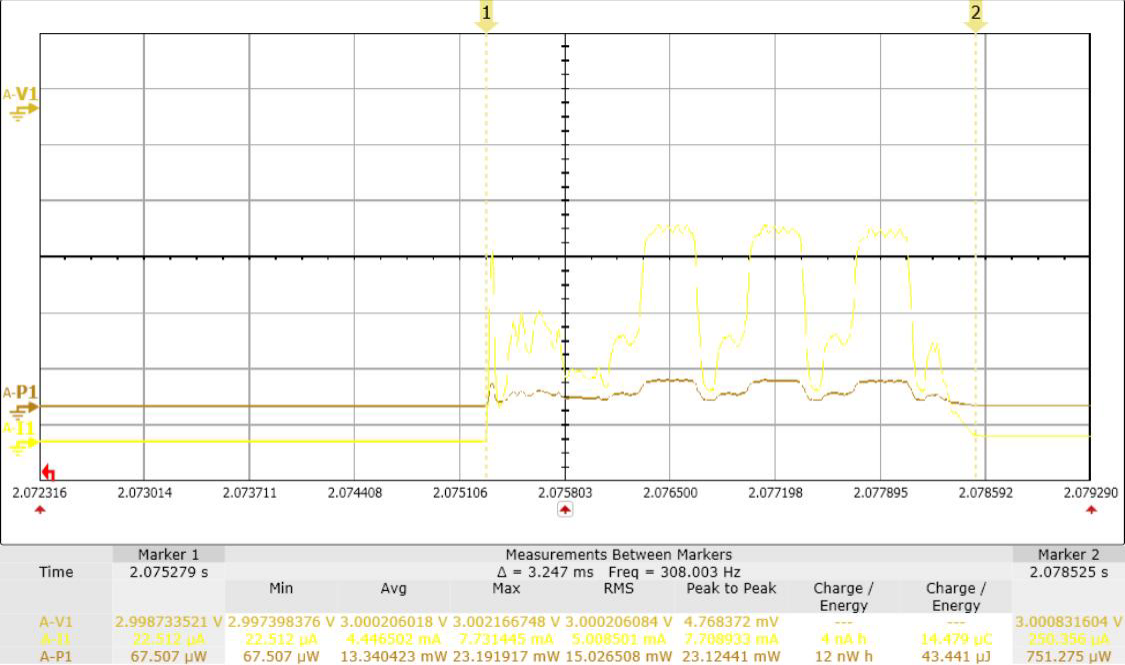
\includegraphics[width=1.0\textwidth]{3Vorgehen/imag/Senden.png}
  \caption{Energieverbrauch senden eines BLE-Paketes mit Sensordaten}
  \label{energie_senden}
\end{figure}


\clearpage

Die Initialisierung ist vergrössert in der Abbildung  \ref{energie_init} dargestellt. Im Überblick geht sie unter, da die Initialisierung direkt ans Laden der TI-SensorTag-Kondensatoren folgt. Da der Peak des Ladens viel höher ist, erscheinen die nachfolgenden Enerigeverbrauche nicht deutlich. Die Energiemessungen einzelner Stellen zeigen, dass für die Initialisierung 77.38 $\mu$J, für das Refreshen ca. $1.4\mu$J (Abbildung \ref{energie_refresh}) und für das Senden des BLE-Pakets (Abbildung \ref{energie_senden}) 43.44 $\mu$J verbraucht werden. Das Senden des BLE-Paketes ist bei der Zeitmarke 2.07 s.


\subsubsection*{Energieverbrauch Starten des Drucksensors}

Auf dem TI-SensorTag wird der Drucksensor BMP 208 von Bosch Sensortec verwendet. Bei der Zeitmarke 1.34 s wird der Sensor gestartet. Die Abbildung \ref{energie_drucksensor} dokumentiert einen Energieverbrauch von 5.753 $\mu$J zum Starten des Sensors.

\begin{figure}[ht]
  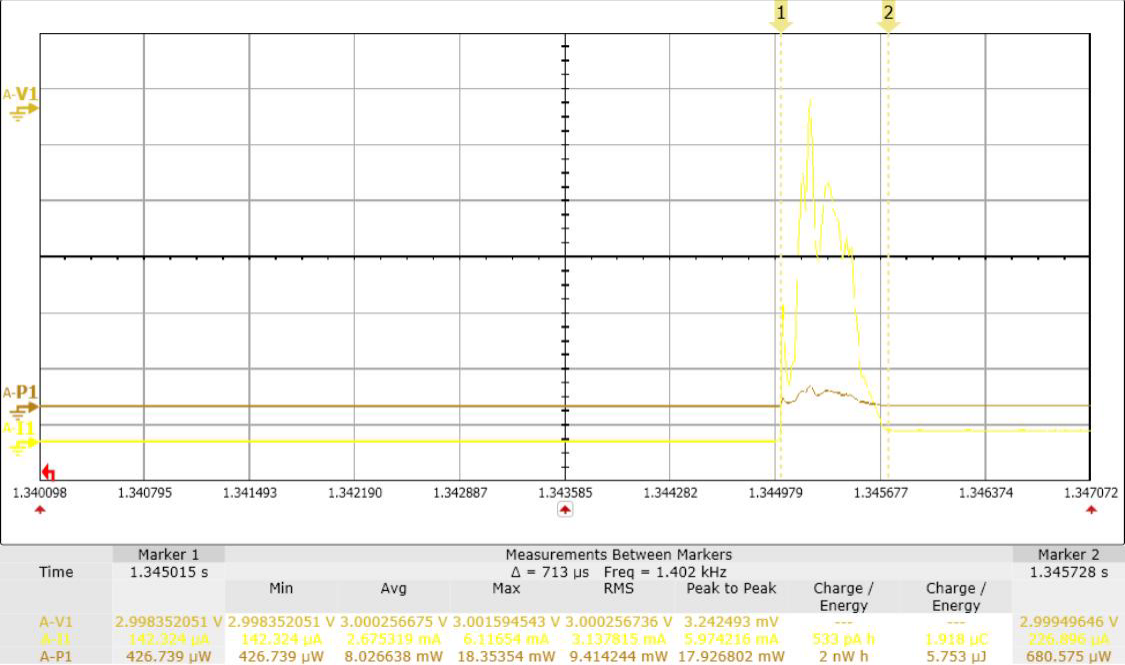
\includegraphics[width=1.0\textwidth]{3Vorgehen/imag/Drucksensor.png}
  \caption{Energieverbrauch des Drucksensors BMP 280}
  \label{energie_drucksensor}
\end{figure}

\clearpage

\subsubsection*{Energieverbrauch beim Starten des Temperatursensors}

\todo{tempsensor daten}
Der Temperatursensor TMP0007 von Texas Instruments verbraucht für das Starten 10.635 $\mu$J. Dies findet bei der Zeitmarke t = 1.54 s statt.

\begin{figure}[ht]
  \includegraphics[width=0.7\textwidth]{3Vorgehen/imag/tempSensor.png}
  \caption{Energiemessung Temperatursensor auf TI-SensorTag}
  \label{energie_tempsensor}
\end{figure}

\subsubsection*{Energieverbrauch Feuchtigkeitssensor}

Der Feuchtigkeitssensor HDC1000 der Marke Texas Instruments verbraucht 6.358 $\mu$J, siehe Abbildung \ref{energie_humidity}.

\begin{figure}[ht]
  \includegraphics[width=0.7\textwidth]{3Vorgehen/imag/Humidity.png}
  \caption{Energieverbrauch Feuchtigkeitssensor}
  \label{energie_humidity}
\end{figure}

\enlargethispage*{15cm}

\clearpage
Um die verschiedenen Energiewerte in Bezug zueinander zustellen, werden in der Tabelle \ref{tab_zsm} die Energiewerte zusammengesfasst und in der Abbildung \ref{energie_zsm} der Verbrauch aller Aktionen in Bezug zueinander graphisch dargestellt. 

%%%%%%%%%%%%%%%%%%%%%%%%%%%%%%%%%%%%%%%%%%%%%%%%%%%%%%%%%%%%%%%%%%%%%%%%%%%%%%%%%%%%%%%%%%%%%%%%%%%%%%%%%%%%%%%%%%%%%%%%%%%%%%%%%%%%%%%%%%%%%%%%

\begin{minipage}{\textwidth}
\captionof{table}{Zusammenfassung Energieverbrauch nach Aktion}
\label{tab_zsm}
\begin{tabbing}
    Aktion \hspace{6cm}                       \quad\= Energie \\[0.8ex]
    Laden C TI-Sensortag            \> 63 $\mu$J \\
    Initialisierung TI-Sensortag    \> 77 $\mu$J \\
    Refresh-Peaks während 10 s      \> 14 $\mu$J \\
    Starten Drucksensor             \> 6 $\mu$J \\
    Starten Temperatursensor        \> 11  $\mu$J \\
    Starten Feuchtigkeitssensor     \>  6 $\mu$J \\
    Senden BLE-Paket nur Geschwindigkeit\> 33 $\mu$J\\
    Senden BLE-Paket mit Sensordaten   \> 43 $\mu$J \\
\end{tabbing}
\end{minipage}

\todo{Einfügen Space in Tabelle}

\begin{figure}[ht]
  \includegraphics[width=1.0\textwidth]{3Vorgehen/imag/Energy_pro_Aufgabe.png}
  \caption{Energieverbrauch pro Aufgabe}
  \label{energie_zsm}
\end{figure}

Es wird deutlich, dass die Initialisierung und das notwendige Refreseshen des Speichers zusammen (die Balken sind violett)  fast gleich viel Energie brauchen, wie das Senden zweier BLE-Pakete mit Sensorwerten. Aus diesem Grund hat erste Priorität beim Power Management, dass die Speisung V\_SUP nicht abstellt. Denn wenn bei der Datenverarbeitung zu viel Energie verbraucht wird und dadurch die Kondensatoren unter den minimalen Schwellwert fallen, fällt die Speisung aus. Jedes Mal wenn die Speisung unterbrochen wird, ist eine neue Initialisierung notwendig. Diese verbraucht unnötig viel Energie.


% x.2 ---------------------------------
\subsection{Energiekalkulation}
\label{v_e_kalkulation}

Die Energiekalkulation dient der Bestückung des Kondensators STS und der Definition von Schwellwerten für die Register im EM8500-Chip. Es wird vom schlechtesten  Fall, also einer Geschwindigkeit von 10 km/h, und dem noch nicht optimalen Energieverbrauch des TI-Sensortags V4 ausgegangen. Laut Datenblatt des EM8500 (\cite{datasheet_EM85}, S.\,9, Abschnitt Operating Conditions ) soll STS zwischen 10 - 100 $\mu$F gross sein. Typisch ist 47 $\mu$F. Die Grundlagen zur Energiekalkulation sind im Theorieteil \ref{th_energiebilanz} abgebildet. Als oberer Schwellwerte beim STS wird 3 V angenommen. Die Berechnung dazu findet sich in der Gleichung \ref{eq:bat_min_low_schwellwert}. 


\todo{Gleichungen als Referenz einbauen}

\begin{flalign}\label{eq:e-high-e-low}
  E_{Applikation} &= E_{Laden C} + E_{Init} + E_{Refreshen}+ E_{Start Drucksensor} + E_{Senden BLE} \\\nonumber
       &= 63\, \mu J + 77\, \mu J + 14\, \mu J+ 6\, \mu J + 43\, \mu J = 203\, \mu J\nonumber
\end{flalign}

\begin{flalign}\label{eq:e_sts}
  C_{STS} &= \frac{2\times 203\, \mu J}{3^2 - (2.1)^2}\\
          &= \frac{ 406\, \mu J}{9 - 4.41}\\\nonumber
          &= \frac{ 406\, \mu J}{4.59}\\\nonumber
          &= 88.45\, \mu F
\end{flalign}

Der Wert wird aufgerundet auf 100 $\mu$F, um genügend Energie zu haben.

\subsubsection*{MPP einstellen}

Während der Entwicklung des Harvesters wurde die Leistungskurve aufgenommen (siehe Messprotokoll \cite{messung_harvester_finish}). Wie im Theorieteil \ref{harv_diff} erklärt unterscheidet sich das Leistungsmaximum nach Geschwindigkeit. Weil das Ziel ein funktionstüchtiger Prototyp bei 10 km/h ist, bezieht sich das Einstellen auf dieses Leistungsmaximum.\todo{Werte überprüfen, aus welchem Messprotokoll kommen die Werte?} Das Leistungsmaximum liegt beim entwickelten Bicycle Computer bei 21.87  $\mu$W. Die MPP-Ratio liegt beim MPP bei 24.87\thinspace\% (siehe \todo{Referenz einbauen}). Die MPP-Ratio liegt somit unter 50\thinspace\%. In der Umsetzung eines Energy Managements mit dem EM8500-Chip ergibt sich das Problem, dass nur Konfigurationen von MPPT-Ratios von 50 - 80\thinspace\% erlaubt sind (siehe Tabelle unten). Zudem sind die Einstellungsschritte der tieferen MPP-Ratio von 50\thinspace\% bis 67\thinspace\% gröber als die von 71\thinspace\% bis 88\thinspace\%. Dies, weil der EM8500-Chip für Harvester vom Typ TEG (ein konstantes MPP bei 50\thinspace\%) und Solarzellen konzipiert ist. Bei der Bewegungsinduktion ist dieser vorgegebene Range nicht ideal.

\begin{minipage}{\textwidth}
    \captionof{table}{MPPT-Ratio Einstellungen EM8500}
    \begin{tabbing}
    Registerwert   \quad\= MPPT-Ratio    \\[0.8ex]
    0x00           \> 50\thinspace\% \\
    0x01           \> 60\thinspace\%\\
    0x02           \> 67\thinspace\%\\
    0x03           \> 71\thinspace\%\\
    0x04           \> 75\thinspace\%\\
    0x05           \> 78\thinspace\%\\
    0x06           \> 80\thinspace\% \\
    0x07           \> 82\thinspace\%\\
    0x08           \> 83\thinspace\%\\
    0x09           \> 85\thinspace\%\\
    0x0A           \> 86\thinspace\% \\
    0x0B           \> 87\thinspace\%\\
    0x0C           \> 88\thinspace\%\\
    \end{tabbing}
\end{minipage}

\todo{Sitzungsprotokoll Datum}

% x.3 -------------------------------------
\subsection{Einstellen der Schwellwerte}
\label{v_schwellwerte}

Das Konzept der Schwellwerte von VSTS und VLTS sind im Theorieteil bei der Erklärung des Speicherkonzepts des EM8500-Chips im Unterkapitel \ref{speicher_konzept} beschrieben. Das Ziel ist, dass sich LTS bei 10 km/h entlädt. Die Berechnung der Schwellwerte stammt aus dem Theorieteil \ref{th_energiebilanz}.

Aus der Vorgängerarbeit sind in der Tabelle unten notierte Konfigurationswerte überliefert. Bei der Inbetriebnahme fiel der hohe Schwellwert von v\_bat\_min\_hi\_dis auf (3.6 V), ab der erst die Applikation gespiesen wird. Der hohe Wert beruht auf dem Versuch, möglichst viel Energie vor dem Datensenden zu sammeln. Ein hoher Schnellwert verzögert die Zeit bis zum ersten Datensenden. Die Vorgänger wählten in ihren Einstellungen eine MPPT-Ratio von 88\thinspace\%. Die Vermutung liegt nahe, dass keine Leistungskurve des Harvesters im Voraus aufgenommen wurde.

\begin{minipage}{\textwidth}
    \captionof{table}{Konfiguration Vorgängermodell}
    \begin{tabbing}
    Register \hspace{4cm} \quad\= Wert \\[0.8ex]
    v\_bat\_max\_hi       \> 4.2 V \\
    v\_bat\_max\_lo       \> 4.1 V \\
    v\_bat\_min\_hi\_dis  \> 3.6 V \\
    v\_bat\_min\_hi\_con  \> 2.1 V \\
    v\_bat\_min\_lo       \> 1.8 V \\
    v\_appl\_max\_hi      \> 3.8 V \\\
    v\_appl\_max\_lo      \> 3.7 V \\ 
    mppt\_ratio            \> 88\thinspace\% \\
    \end{tabbing}
\end{minipage}

Nach der Energiemessungen der Version V3 des TI-SensorTags (siehe \ref{erst_EMessungen}), in dem die Geschwindigkeit per BLE gesendet werden kann, entstanden folgende Schwellwerte:

\begin{minipage}{\textwidth}
    \captionof{table}{Konfiguration aufgrund Geschwindigkeitsmessung}
    \begin{tabbing}
    Register\hspace{4cm} \quad\= Wert \\[0.8ex]
    v\_bat\_max\_hi       \> 4.8 V \\
    v\_bat\_max\_lo       \> 4.7 V \\
    v\_bat\_min\_hi\_dis  \> 2.8 V (siehe Berechnungen unten)\\
    v\_bat\_min\_hi\_con  \> 2.1 V \\
    v\_bat\_min\_lo       \> 2.0 V (vorgegeben von TI-SensorTag)\\
    v\_appl\_max\_hi      \> 3.8 V \\\
    v\_appl\_max\_lo      \> 3.7 V \\ 
    mppt\_ratio            \> 50\thinspace\% (aus MPP-Kurve Harvester)\\
    \end{tabbing}
\end{minipage}

Die Grundlage bildete die Gleichung  $E_{Applikation}= E_{STS\_HIGH} - E_{STS\_LOW}$ \todo{Referenz Theorie}, wobei  $E_{Applikation}$ aus der Messung von V4 mit total 189 $\mu$J für die Initialisierung und das Senden der Daten gebraucht werden. Als Kondensatorwert für STS wird 100 $\mu$F genommen. So ergibt sich folgender minimaler oberer Schwellwert:

\begin{flalign}\label{eq:bat_min_low_schwellwert}
    (v\_bat\_min\_low) ^2  &=  \frac{2\, \times \, E_{Applikation}}{C_{STS}} + (V_{STS\_LOW})^2\\
     &=  \frac{2\, \times \, 189, \mu J}{100 \,\mu F} + (2.0 V)^2\\ \nonumber
    v\_bat\_min\_low  &=  \sqrt{\frac{378 \,\mu J}{100 \,\mu F} + 4 V^2} = \sqrt{7.8 V^2} = 2.79 V \\\nonumber
\end{flalign}

Wichtigster Wert in der Konfiguration ist jedoch der korrekte MPPT-Wert. Er wird auf das Minimum (50\thinspace\%) gesetzt. Das Maximum des Ladezustands  wird auf den maximal erlaubten Wert gesetzt: v\_bat\_max  = 4.8 V bzw. 4.7 V. Denn solange Energie geerntet werden kann, soll sie gespeichert werden. v\_appl\_max spielt in unserer Anwendung keine wichtige Rolle. Der Wert wird von den Vorgängern übernommen.

Das Zusammensetzen der Last (TI-SensorTag) mit der konfigurierten Hardware erstaunte (siehe Messprotokoll \cite{messung_inbetrieb_prototyp}). Ab 25 km/h funktionierte die Schaltung gut. Doch darunter reagiert der EM8500-Chip nicht. Weder STS noch LTS konnten sich laden. Nachmessungen am Eingang vom EM8500-Chip ergaben, dass bei  10 km/h und einer MPPT-Ratio von 50\thinspace\% eine Spannung von 0.2 V anliegt. Diese ist zu tief, um den Booster zu starten. Erst bei höherer Geschwindigkeit wird eine Eingangsspannung von mehr als 0.3 V erreicht, und das System beginnt zu funktionieren. Um eine Minimalspannung von 0.3 V bei niedrigen Geschwindigkeit zu garantieren wird die MPPT-Ratio zukünftig auf den zweittiefsten Wert (60 \thinspace\%) eingestellt.

Ein unerwartetes Verhalten des Drucksensors zeigt sich bei der Implementation des Auslesens. Der BLE-Sniffer empfängt die Druckdaten korrekt, doch beim Anschliessen des TI-SensorTags an die Harvesterschaltung, riss die Spannung sofort zusammen. Innert kürzester Zeit entlädt sich der STS sowie der parallel geschaltene LTS. Unterschreitet der STS den Schwellwert von V\_SUP von 2 V, so stellt die Speisung der Applikation ab (siehe Abbildung \ref{i2c_problem} im Unterkapitel \ref{erst_EMessungen}). Das Ausmessen des Energieverbrauchs bringt Klarheit: Die I2C-Kommunikation und das Aufstarten des Sensors brauchen xxx-mal mehr Energie als das Berechnen der Geschwindigkeit aus den Reed-Switch Impulsen (siehe Abbildung \ref{r_bild_e_zusammenfassung}\todo{Referenz überprüfen} im Resultat-Teil).

\todo{Faktor ausrechnen}

Durch den deutlich höheren Energieverbrauch wird eine Power-Optimierung im Softwareteil notwendig. Es zwingt aber auch dazu, den Schwellwert von v\_bat\_min\_hi\_dis  wieder zu erhöhen. Die finale Konfiguration ist im Resultate-Teil abgebildet.


% x.4 -----------------------------------------
\subsection{Energiezustand des Systems}
\label{v_energiezustand}

Die letzte der vier Aufgaben aus der Optimierungsliste nach der Inbetriebnahme (siehe Unterkapitel \ref{optimierung}) ist das variable Anpassen des BLE-Paketsendens aufgrund des Energiezustandes. Im ersten Unterkapitel \ref{def_zustaende} wird das Einteilen des Systems in Energiezustände beschrieben. %, danach die Umsetzung wie in Software das Auslesen und Verarbeiten der Energiezustände angewendet wird. 

\todo{Umsetzung in Software ev. dazu}

\subsubsection*{Definition von Energiezuständen}
\label{def_zustaende} 

Da die produzierte Energie von der Fahrgeschwindigkeit abhängt, werden die Energiezustände aufgrund der Fahrgeschwindigkeit definiert. Welche Aufgaben in welchem Energiezustand erledigt werden, folgt in den Abbildungen \ref{LOW_ENER}, \ref{MID_ENER} und \ref{HIGH_ENER}, direkt nach der Definition der Zustände. 

\begin{minipage}{\textwidth}
    \captionof{table}{Energiezustände aufgrund der Geschwindigkeit}
    \begin{tabbing}
       Geschwindigkeit\quad\= Systemzustand\\[0.8ex]
       0 - 15 km/h        \> LOW\_ENERGY\\
       15 - 20 km/h       \> MIDDLE\_ENERGY\\
       $>$ als 20 km/h    \> HIGH\_ENERGY\\    
    \end{tabbing}
\end{minipage}

Bei wenig Energie lädt sich nur der STS. Erreicht er den Schwellwert für die Speisung der Applikation, so erhält TI-SensorTag Spannung. Die Reed-Impulse werden ausgelesen, der zweite Prozessor für das Senden der BLE-Pakete gestartet und die Daten übertragen. Bei wenig Energie verbrauchen diese drei Aktionen sämtliche zur Verfügung stehende Energie. Denn LTS hat sich nicht geladen. Die Energie genügt nicht für weitere Aktionen.

\begin{figure}[ht]
    \begin{minipage}[t]{0.5\textwidth}
      \includegraphics[width=1.0\textwidth]{3Vorgehen/imag/LOW_ENERGY.png}
      \caption{Wenig Energie}
      \label{LOW_ENER}
    \end{minipage}
    \begin{minipage}[t]{0.5\textwidth}
      \includegraphics[width=1.0\textwidth]{3Vorgehen/imag/MIDDLE_ENERGY.png}
      \caption{Mittlere Energie}
      \label{MID_ENER}
    \end{minipage}
\end{figure}

Bei etwas mehr Energie befindet sich das System in einem Zwischenzustand (Abbildung \ref{MID_ENER}). Zu jeder Geschwindigkeitsmessung wird ein Sensor ausgelesen. Im Idealfall unterstützt LTS die Stabilität. Wenn nicht, schaltet V\_SUP bei zu wenig Energie ab. Im hohen Energiezustand werden mit jedem Geschwindigkeitspaket die aktualisierten Werte der drei Sensoren mitübertragen. 

\begin{figure}[ht]
  \includegraphics[width=0.45\textwidth]{3Vorgehen/imag/HIGH_ENERGY.png}
  \caption{Viel Energie}
  \label{HIGH_ENER}
\end{figure}


% 4 ---------------------------------------------------------------------------
\section{Power Management}
\label{powerOptimierung}

Das Power Management wird mit dem TI-SensorTag umgesetzt. Im ersten Unterkapitel \ref{keinROTS} wird beschrieben, auf welche Bibliotheken und Hilfen man von Texas Instruments zurückgreifen kann. In nächsten Unterkapitel \ref{PowerDomains} werden die Power-Domains des TI-SensorTags erklärt und im letzten Unterkapitel die Umsetzung, z.B. wie Schlafenszeiten eingebaut werden \ref{sleep_funktion}.


\subsection{Programmieren für Low Power Applikation im Adevertising Mode}
\label{keinROTS}

Das ausgewählte TI-SensorTag ist für Low-Power-Anwendungen ausgelegt. Die Low-Power-Programmbeispiele von TI basieren auf dem TI-Real Time Operating System (kurz RTOS). Da bei 10 km/h Energie im $\mu$J-Bereich zur Verfügung steht, läuft die Applikation im Advertising Mode. Dieser braucht weniger Energie als der Connected Mode und der Overhead eines Betriebsystems (RTOS) und der Initialisierung des BLE-Stacks sind nicht notwendig. Der Nachteil dieser schlanken Programmierung ist, dass die TI-SensorTag Beispiele ausschliesslich auf RTOS aufbauen, und somit nicht 1:1 übernommen werden können. Für nachkommende Entwicklerinnen und Entwickler sind zwei Vorzüge und zwei Nachteile dieser Wahl festgehalten:

\begin{minipage}{1\textwidth}
    \begin{enumerate}
        \item Vorteil ohne RTOS: Ein sehr schlanker Code entsteht. Die Register werden direkt gesetzt, und die Funktionsaufrufe sind sehr schnell.
        \item Vorteil ohne RTOS: Man muss sich nicht in das TI-RTOS-Konzept einarbeiten. Die Message-Queue und das Thread-Handling bei TI muss man nicht kennen.
        \item Nachteil ohne RTOS: TI implementierte über die Library die Hauptaktivitäten wie Power Domains einschalten oder Kommunikation zu Peripheriegeräten aufbauen. Die Zugriffe werden vom OS übernommen. Ohne RTOS muss man sich selber z.B. ums Aufwachen oder das Abhandeln der Interrupts kümmern.        
       \item Nachteil ohne RTOS: Eine Dokumentation zur umfangreichen Library (cc26xxware/driverLib) fehlt, da TI davon ausgeht, dass man über das OS auf die Bibliothek zugreift. Die internen Abhängigkeiten zu verstehen, ist nicht einfach. Unerwünschte Nebeneffekte treten auf.
    \end{enumerate}
\end{minipage}

\subsection{Power Domains beim TI-SensorTag}
\label{PowerDomains}

Bei einer Low Power Applikation hat das Ein- und Ausschalten von sogenannten Power Domains eine zentrale Rolle. Das TI-SensorTag unterscheidet 10 Power Domains. Ein Überblick  ist in der Abbildung  \ref{supply_syst} abgebildet. Das Konzept der Verbrauchsoptimierung besteht im Abschalten unnötiger Peripherie- und Prozessorteilen. Nur absolut notwendige Power Domains laufen weiter. Der Teil, der nicht abstellt wird, wird AON (Always On) genannt. Zu dieser Domain gehört ein Clock, ein Timer, gewisse Interrupts und Schnittstellen. Im Anhang \ref{anhang_sensortag_PowerDomain} ist in der Abbildung \ref{a_powerdomain} detailliert dargestellt, wie die einzelnen Power Domains sich beim Ausschalten verhalten. So braucht z.B. das RAM und die GPIO Refreshzyklen. Beim RAM bedeutet dies eine Speicherauffrischung, bei der GPIO eine Kontrolle der Pinzustände.

\clearpage
\begin{figure}[ht]
  \includegraphics[width=1.0\textwidth]{3Vorgehen/imag/powerdomain_1.png}
  \caption{Supply System TI-SensorTag aus: \cite{Sensortag_Manual}, S.\,416}
  \label{supply_syst}
\end{figure}


\subsection{Schlafenszeiten implementieren}
\label{sleep_funktion}

In der Theorie wird das Schlafen zwischen Funktionsblöcken beschrieben \ref{pm_sleep}. Der Energy Managements-Teil fasst zusammen, welche Aktionen bei welcher Energie gemacht werden können (siehe Abbildungen \ref{warten_zw_bloecken}\todo{referenz überprüfen}). Das Auslesen der Sensoren ist nur möglich, weil die Aktionsblöcke aufgeteilt werden und das System dazwischen Schlafen geht. Die Abbildung \ref{warten_zw_bloecken} zeigt den implementierten Codeablauf der TI-SensorTag Version V4, bei einer Geschwindikeit unter 50 km/h \todo{Geschwindikeit überprüfen}. Der Fall von einer Geschwindigkeit von über 50 km/h\todo{Geschwindikeit überprüfen}, bei der V\_SUP nicht mehr abstellt, ist im letzten Unterkapitel illustriert.

\begin{figure}[ht]
  \includegraphics[width=0.5\textwidth]{3Vorgehen/imag/schlafen_funktionen.png}
  \caption{Schlafenszeiten zwischen Aktionen}
  \label{warten_zw_bloecken}
\end{figure}

Ist eine Aufgabe getätigt, wie z. B. das Starten eines Sensors, kann das System schlafen gehen. Dieses Prozedere funktioniert einwandfrei und sicher. Das System wacht aufgrund eines Interrupts wieder auf. Nachfolgend sind die zwei Hauptfunktionen: Vorbereiten zum Standby und ausschalten des Hauptprozessor abgebildet.

\subsubsection{Standby-Prozedur}
\label{vorbereiten}

Die abgebildete Funktion verdeutlicht exemplarisch, welche Schritte bei einer Programmierung ohne RTOS durch die Programmiererin bzw. den Programmierer ausgeführt werden.  Zum Verständnis werden einige Zeilen des Codes kurz kommentiert:\\ 

Zeile 2:\hspace{1cm}   Der Crystal-Oszillator wird abgeschaltet,\\
Zeile 3:\hspace{1cm}   Das Radio-Modul ebenfalls,\\ 
Zeile 4:\hspace{1cm}   Ein niedriger Takt wird eingestellt und\\ 
Zeile 5:\hspace{1cm}   unnötige Peripheriespeisung abgestellt.\\ 
Zeile 6:\hspace{1cm}   Dem Prozessor wird erlaubt, seine notwendigen Register zu refreshen und\\ 
Zeile 7:\hspace{1cm}   das Cache wird abgeschaltet.\\ 
Zeile 8:\hspace{1cm}   Wobei ein Refreshzyklus aktiviert wird.\\
Zeile 11:\hspace{1cm}  Das Intervall zwischen den Refreshzyklen wird berechnet\\
Zeile 12:\hspace{1cm}  Es wird gewartet, bis alle Anweisungen abgeschlossen sind\\


\todo{Leerzeile einbauen}

\begin{minipage}[t]{1\textwidth}
\small\begin{verbatim}
1    void go_to_standby(){ 
2        powerDisableXtal();
3        powerDisableRFC();
4        OSCHfSourceSwitch(); // activates lower clock
5        powerDisableAuxForceOn();
6        powerEnableMcuPdReq();
7        powerDisableCache();
8        powerDisableCacheRetention();
9
10        // calculate next recharge time
11        SysCtrlSetRechargeBeforePowerDown(XOSC_IN_HIGH_POWER_MODE);
12        SysCtrlAonSync();
13    } 
    \end{verbatim}\normalsize
\end{minipage} 	    

\subsubsection{Abschalt-Prozedur}
\label{ausschalten}

Nach der Vorbereitung zum Abschalten wird der Prozessor zum Schlafen geschickt.\\

Zeile 2:\hspace{1cm}   Cortex M3 wird zum Schlafen geschickt\\
Zeile 3:\hspace{1cm}   Das Power-Control-Register erhält das Schlafens-Flag\\
Zeile 4:\hspace{1cm}   Die Always-On-Power-Domain muss die Konfigurationen speichern\\
Zeile 5:\hspace{1cm}   Den Refrehzyklus-Wert setzen\\
Zeile 6:\hspace{1cm}   Warten, dass alle Prozesse fertig abgehandelt sind.\\

\begin{minipage}[t]{1\textwidth}
\small\begin{verbatim}
1    void go_to_deep_sleep(){ 
2        powerDisableCPU();
3        PRCMDeepSleep();
4        SysCtrlAonUpdate();
5        SysCtrlAdjustRechargeAfterPowerDown();
6        SysCtrlAonSync();
7    }
\end{verbatim}\normalsize
\end{minipage}

\subsubsection{Sleep Time-Übersicht bei Version V4}
	    
Bei den ersten Messungen von Sensoren riss V\_SUP so schnell zusammen, dass kein BLE-Paket gesendet wird \todo{Link}. Das Senden wird möglich, indem zwischen einzelnen Aufgaben geschlafen wird. Denn während dem das TI-SensorTag nur die minimale Energie verbraucht, kann der Bicycle Computer Energie sammeln. Während der Schlafenszeit steigt der Spannungswert an den Kondensatoren STS und LTS. Die Abbildung \ref{schnarch} zeigt, dass bei der Version V4 (siehe xxxx \todo{Link zu Sensortag versionen einbauen} die Aufgaben aufteilt werden. Dies entspricht dem Konzept des vorangehenden Unterkapitels mit der Abbildung \ref{warten_zw_bloecken}, nur dass in Abbildung \ref{schnarch} der Fall von einer Geschwindigkeit von über 40 km/h \todo{Wert prüfen} gezeigt wird, und V\_SUP deshalb nicht abstellt.   

Beim Senden von Sensordaten sind zwei Funktionen kritisch: das Starten eines Sensors und das Senden der Daten. Diese zwei Aufgaben werden getrennt und dazwischen geht das System schlafen (siehe vereinfacht dargestellt in der Abbildung \ref{schnarch}).

\begin{figure}[ht]
  \includegraphics[width=1.0\textwidth]{3Vorgehen/imag/HIGH_ENERGY.png}
  \caption{Auftrennen der Arbeit durch Schlafen dazwischen}
  \label{schnarch}
\end{figure}


Die Schlafenszeit wird experimentell ermittelt. Innerhalb des GPIO-Handlers zählt ein Counter die Reed Switch-Interrupts, also die Radumdrehungen. Da am Fahrrad zwei Magnete befestigt sind, entspricht der Counterwert der doppelten Anzahl Radumdrehungen. Ist  das Zählermaximum erreicht, wird der Code rund um eine energiestarke Aktion ausgeführt. Danach geht das System schlafen. Das System soll so lang schlafen, dass die Spannung von V\_STS genug gross ist, dass die energiestarke Aktion ausgeführt werden kann. In der unten aufgeführten Tabelle findet sich eine grobe Count-Statistik der Version V4 für verschiedene Geschwindigkeiten. 

\begin{minipage}{\textwidth}
    \captionof{table}{Zählerstände für Schlafenszeit}
    \begin{tabbing}
   Geschwindigkeit \quad\= Counter-Wert  \quad\= Ladezeit STS    \quad\= Radumdrehungen\\[0.8ex]
   13 - 16 km/h          \> 100               \> 80 s    \> 50\\
   20 km/h               \> 50                \> 17 s    \> 25\\
   31 - 32 km/h          \> 50                \> 11 s    \> 25\\    
    \end{tabbing}
\end{minipage}

Das Setzen der Schlafenszeit ist einer globalen Variable gespeichert. Abhängig von der Geschwindigkeit, wird das Schlafensintervall (das Counter-Maximum) angepasst.






% 5 ---------------------------------------------------------------------------
\section{Applikationsentwicklung}
Nachfolgend wird der Aufbau von TI SensorTag zusammen mit unserem selbst entwickelten Board als Sensor benannt und die Android Applikation auf dem Smartphone wird einfach als Applikation benannt.

\subsection{Aufbau der Applikation}

\begin{figure}[ht]
    \includegraphics[width=0.5\textwidth]{3Vorgehen/imag/Aufbau_Applikation_erste_Version.png}
    \caption{Aufteilung des Bildschirms}\label{aufbau_applikation_1} 
\end{figure}

Der Aufbau der Applikation sollte am Anfang in vier Teile des Bildschirms geteilt werden (siehe Abbildung \ref{aufbau_applikation_1}). 
Im Bereich GPS soll eine Karte angezeigt werden. Ausserdem soll es möglich sein die Route aufzuzeichnen und abzuspeichern.
Der Verlauf zeigt die Entwicklung der Geschwindigkeit über einen gewissen Zeitraum, wobei es wählbar sein soll welche Daten angezeigt werden.
Die Geschwindigkeit soll anschaulich in einem Tachometer angezeigt werden und die Tachonadel soll im besten Fall animiert sein.
Im Bereich der Werte sollen die aktuellen Werte in Zahlen und den entsprechenden Einheiten dargestellt werden.
Schnell wurde klar, dass dieser Aufbau wenig Sinn macht, da die Bereiche auf einem Smartphone viel zu klein wären und nicht mehr leserlich sein würden. Darum wurden die Teile des Bildschirms als einzelne Activities geplant, somit wäre der ganze Bildschirm als Anzeige für jede einzelne Aufgabe vorhanden.

\subsubsection{Home-Screen}

Als erstes soll der Benutzer den sogenannten Home-Screen sehen, hier werden der Tachometer, die Werte und Buttons zur Bedienung angezeigt. Je nach Anzahl der Funktionen sollen neue Buttons implementiert werden. So soll beispielsweise für die Sensorwahl ein Button vorhanden sein. Während der Entwicklung der Applikation wurde die Idee von einer GPS-Karte und einem Verlauf verworfen, da diese Funktionen aus zeitlichen Gründen nicht mehr realisierbar waren.

\subsubsection{Sensorwahl}

Schnell wurde klar, dass die Auswahl eines spezifischen Sensors wichtig werden würde, für den Fall, dass einmal mehrere Sensoren vorhanden wären. Ein Beispiel: Würde unsere Applikation bei einem Fahrradrennen eingesetzt werden, so müsste die Applikation auf dem Smartphone mit dem Sensor am Fahrrad gepaart werden. Ansonsten würde man die Daten von allen Sensoren empfangen und die Anzeige würde nicht die Daten des eigenen Sensors anzeigen.

\subsubsection{Einheiten und Einstellungen}

Es kam ebenfalls der Wunsch auf, die Einheiten der Werte einstellbar zu machen, da die Applikation bestenfalls auch in anderen Ländern verwendet werden soll. Also wäre es optimal, wenn die Geschwindigkeit beispielsweise auch in Miles per Hour dargestellt werden könnte. Es müsste eine Einstellungsmöglichkeit bereitgestellt werden, damit die Temperatur kalibriert werden kann.

\subsubsection{BLE-Kommunikation}

Der wichtigste Teil der Applikation ist die Bluetooth-Kommunikation. Hier werden die Daten vom Sensor empfangen. Die Daten müssen nach dem Empfangen gefiltert werden, damit sichergestellt wird, dass die empfangenen Daten von einem unserer Sensoren kommen. Sobald sichergestellt ist, dass die empfangenen Daten zu unserem Sensor gehören, müssen diese umgerechnet werden.

\subsubsection{Inbetriebnahme des Codes der PA}

Als erster Schritt wurde der Code der vorangegangenen Arbeit analysiert und die wichtigen Teile zur Bluetoothkommunikation übernommen. Es wurden folgende Funktionen aus dem Code übernommen: onStart, onActivityResult, scanLeDevice, BluetoothAdapter.LeScanCallback.

Die Funktion onStart wurde in BLE\_init umbenannt und der Mechanismus zum Wachhalten des Geräts wurde entfernt. Der Mechanismus wurde entfernt, da dieser nicht mehr funktionierte. Ebenfalls wurde die Funktion in die Funktion onCreate eingefügt, um den Code übersichtlicher zu gestalten und da diese Funktion nur einmalig aufgerufen werden musste.
 
Die Methoden onActivityResult und scanLeDevice wurden komplett übernommen.

Die Callback-Funktion des Bluetoothadapters BluetoothAdapter.LeScanCallback wurde strukturell übernommen, jedoch wurde die Codierung zur Verarbeitung der Daten entfernt.

\subsubsection{Filter einbauen}
Der nächste logische Schritt war, dass die empfangenen Daten gefiltert werden mussten. Dafür wurde folgende Struktur definiert, damit festgestellt werden kann, ob die Daten von einem unserer Sensoren versendet wurden.

\todo{tabelle zu lang. kürzen}

\captionof{table}{Filter}
\begin{tabbing}
	Lenth \quad\=		23\\[0.8ex]
	Type\>				0x03\\
	UUID\>				0xDEBA\\
	Package ID\>		2 bytes\\
	Speed\>				4 bytes\\
	Pressure\>			4 bytes\\
	Temperature\>		4 bytes\\
	Humidity\>			4 bytes\\
	Checksum\>			2 bytes\\
\end{tabbing}
Aufgrund dieser Struktur können alle empfangenen Daten, welche nicht die definierte Länge, Typ und UUID besitzen, ignoriert werden.

Wenn sichergestellt ist, dass die Daten von unserem Sensor stammen, musste noch die Adresse vom Sender gespeichert werden. Alle Adressen werden in einer Liste gespeichert, vor dem Speichern wird jedoch noch geprüft, ob die Adresse bereits in der Liste ist, falls dies so ist wird die Adresse nicht noch einmal gespeichert.

\subsubsection{Berechnung der Daten}

Der Sensor sendet Werte wie den Zeitunterschied zwischen zwei Magnetdurchläufen, den Luftdruck, die Temperatur und die relative Luftfeuchtigkeit. Diese Daten müssen erst noch in die korrekten Werte umgerechnet werden, da alle Werte in mehreren Bytes verteilt vorliegen.

Der Zeitunterschied zwischen zwei Magnetdurchläufen wird in vier Bytes dargestellt. Die ersten beiden Bytes enthalten die Anzahl Sekunden. Folgende Formel zeigt die Umrechnung von zwei Bytewerten in eine reelle Zahl:

\begin{equation}
	t = ((byte_0 << 8) + byte_1)
\end{equation}

Die erhaltene Zahl muss noch mit einem Typecast in den Datentyp float umgewandelt werden, um die weiteren Berechnungen zu erleichtern.

Das dritte und vierte Byte des übermittelten Zeitunterschieds enthält die Sekundenbruchteile. Folgende Formel zeigt, wie die Bytes verrechnet werden müssen, um die korrekten Werte zu erhalten:

\begin{equation}
	t = \frac{((byte_2 << 8) + byte_3)}{2^{16}}
\end{equation}

Der erhaltene Sekundenbruchteil kann nun zu den ganzen Sekunden dazu addiert werden, um die ganze Zeit zwischen zwei Magnetdurchläufen zu erhalten.

Ein Beispiel: Wird also der hexadezimale Wert 0x00041000 empfangen sind das 1.25 Sekunden zwischen zwei Magnetdurchläufen. Die genaue Berechnung des Beispiels kann in den nachfolgenden Formeln verfolgt werden:

\begin{equation}
	t_{ganze Sekunden} = ((0x01 << 8) + 0x00) = 1 s
\end{equation}

\begin{equation}
	t_{Sekundenbruchteile} = \frac{((0x40 << 8) + 0x00)}{2^{16}} = 0.25 s
\end{equation}

\begin{equation}
	t_{Total} = t_{ganze Sekunden} + t_{Sekundenbruchteile} = 1 s + 0.25 s = 1.25 s
\end{equation}

Um die Geschwindigkeit zu erhalten muss der Radumfang durch die erhaltene Zeit geteilt werden. Jedoch befinden sich an unserem Rad zwei Magnete, deswegen darf nur der halbe Radumfang verrechnet werden. Ausserdem ist das Resultat in m/s und muss deshalb noch in km/h umgerechnet werden, was nichts anderes als eine Multiplikation mit dem Faktor 3.6 ist.

Der Druck wird in Pascal (Pa) übertragen, hier müssen die verschiedenen Bytes miteinander addiert werden und in hPa umgerechnet werden. Es werden jedoch nur die letzten drei Bytes mit Werten befüllt sein, da das TI-SensorTag nur drei Bytes aus dem Drucksensor erhält. Das erste Byte kann ignoriert werden. Trotzdem wurden vier Byte übertragen, um später die Daten zum Druck mit weiteren Informationen zu bestücken. Folgende Formel zeigt die Umrechnung der Bytes in eine float Zahl:

\begin{equation}
	p = (float)((byte_2 << 16) + (byte_1 << 8) + byte_0) \times 0.01
\end{equation}

Die barometrische Höhenformel (\cite{Formelbuch}, Seite 284) zeigt die Abhängigkeit des Druckes von der aktuellen Höhe.

\begin{equation}
	p(h) = p_0 \times e^{-\frac{h}{7991 m}}
\end{equation}

Durch Umformen ergibt sich die folgende Formel, womit sich die Höhe aus dem Druck berechnen lässt.

\begin{equation}
	h = ln(\frac{p(h)}{p_0}) \times (-7991 m) = ln(\frac{p(h)}{1013.25 hPa}) \times (-7991 m)
\end{equation}

Die Temperatur wird in zwei Bytes übertragen. Jedoch wird die Temperatur nicht in $^\circ$C übertragen, sondern in Tausendsteln Grad Celsius. Ein Beispiel: Die Temperatur 23 $^\circ$C wird als 23000 übertragen. Das bedeutet, dass die Temperatur, welche empfangen wird, zusammengesetzt werden muss und durch 1000 dividiert werden muss. Die Formel sieht folgendermassen aus:

\begin{equation}
	T = (float)((byte_1 << 8) + byte_0) \times 0.001
\end{equation}

Der letzte Wert, welcher vom Sensor versendet wird, ist die relative Luftfeuchtigkeit. Die Formel zur Berechnung der relativen Luftfeuchtigkeit sieht folgendermassen aus:

\begin{equation}
	H = (float)((byte_3 << 24) + (byte_2 << 16) + (byte_1 << 8) + byte_0) \times 0.01
\end{equation}


\subsection{Einstellungsmöglichkeiten}

Als nächstes wurde die Aufgabe in Angriff genommen, die Applikation als User einstellen zu können. Es musste genau überlegt werden, welche Einstellungen ein User machen darf und welche dem Programmierer bzw. der Applikation überlassen werden.


\subsubsection{Adressauswahl}

Die Adressauswahl oder auch Sensorwahl ist ein Bedürfnis, da der User die Applikation mit seinem eigenen Sensor paaren können sollte. Es sollte sichergestellt werden, dass die Applikation nach der Sensorwahl nur noch Daten von dem gewählten Sensor anzeigt und die Daten der anderen Sensoren ignoriert werden. Die Adressen von Sensoren in der Nähe sollten aber weiterhin gespeichert werden, damit man gegebenenfalls auch einen anderen Sensor auswählen konnte.

Immer wenn Daten empfangen werden und die Struktur mit der definierten Struktur übereinstimmen soll die Adresse gespeichert werden. Dafür wurde folgende Funktion entwickelt:

\begin{figure}[ht]
    \includegraphics[width=0.8\textwidth]{3Vorgehen/imag/app_saveAdress.png}
    \caption{Sourcecode saveAdress}
	\label{app_saveAdress} 
\end{figure}

Der adressCounter wird mit dem Wert -1 initialisiert. Werden die ersten Daten mit der vorgegeben Struktur empfangen wird die Funktion automatisch die Adresse in der adressList an der Stelle 0 speichern. Werden erneut Daten von einem unserer Sensoren empfangen wird zuerst geprüft, ob die Adresse bereits ein Teil der adressList ist. Falls die Adresse noch nicht in der Liste enthalten ist, wird der Index bzw. der adressCounter, erhöht und die Adresse in der Liste gespeichert.

Sobald eine Adresse ausgewählt wurde, müssen die zukünftigen Datenpakete überprüft werden, ob sie vom ausgewählten Sensor stammen. Die Funktion checkAdress überprüft, ob die ausgewählte Adresse der Adresse des Sensors entspricht, welche die neuen Daten gesendet hat. Sollte keine Adresse ausgewählt sein, so wird dies behandelt, als ob der Sensor die richtige Adresse hat.

\begin{figure}[ht]
    \includegraphics[width=0.8\textwidth]{3Vorgehen/imag/app_checkAdress.png}
    \caption{Sourcecode checkAdress}
	\label{app_checkAdress} 
\end{figure}

Der User muss noch die Möglichkeit haben eine Adresse auszuwählen, dafür wird eine neue Benutzeroberläche (Activity) erstellt. Die neue Activity ist eine List-Activity. Das bedeutet, dass es wird eine Liste von möglichen Adressen angezeigt wird, welche mit einem Klick auf die gewünschte Adresse ausgewählt wird. Anschliessend wird die ausgewählte Adresse an die Haupt-Activity zurückgegeben. In Abbildung \ref{BLEadressauswahl} ist die List-Activity zu sehen, welche eine Adresse zur Auswahl hat. Damit die ausgewählte Adresse von der Haupt-Activity überhaupt empfangen werden kann, musste die List-Activity mit den auszuwählenden Adressen mit folgendem Befehl gestartet werden: startActivityForResult. Die gestartete Activity kann somit ein Resultat, also die ausgewählte Adresse, zurückgeben und die Haupt-Activity kann diese in der Funktion onActivityResult empfangen und abspeichern. Die genaue Ausführung der Übergabe der Adressen sowie die Rückgabe der ausgewählten Adresse kann dem Quellcode entnommen werden.

\begin{figure}[ht]
    \includegraphics[width=0.2\textwidth]{3Vorgehen/imag/BLEAdresseAuswaehlen.png}
    \caption{Adressauswahl mit nur einer Adresse}
	\label{BLEadressauswahl} 
\end{figure}



\subsubsection{Einheiten}

Die Einheiten der empfangenen Daten sollten ebenfalls einstellbar gestaltet werden. Für diesen Zweck wurden mehrere Enumerationen definiert. Die Enumeration für die Temperatur sieht folgendermassen aus:

\begin{figure}[ht]
    \includegraphics[width=0.8\textwidth]{3Vorgehen/imag/app_tempSetting.png}
    \caption{Sourcecode Enumeration}
	\label{app_tempSetting} 
\end{figure}

Es wurden der Enumeration drei Elemente hinzugefügt, welche alle einen Faktor, einen Offset und einen String mit der geschriebenen Einheit enthalten. Anhand dieser Enumeration kann der Faktor und der Offset einfach zugänglich gemacht werden. (\cite{calcTemp})(\cite{calcPressure})(\cite{calcVelocity}) 

Eine neue Activity wurde codiert, welche drei Spinner zur Auswahl der Einheiten, ein Eingabefeld (EditText) für die Eingabe des Radumfangs und ein EditText für die Kalibrierung der Temperatur zur Verfügung stellt. Die eingestellten Einheiten und die eingetragenen Werte werden über den Speichern-Button an die Haupt-Activity zurückgegeben. In der Haupt-Activity werden diese Daten empfangen und abgespeichert und anschliessend zur Darstellung der Werte verwendet. Erst bei der Anzeige der Werte werden die eingestellten Faktoren und Summanden der Enumerationen verwendet.

\begin{figure}[ht]
    \includegraphics[width=0.2\textwidth]{3Vorgehen/imag/onActivityResult.PNG}
    \caption{Datenübergabe zwischen den Activities}
	\label{onActivityResult} 
\end{figure}

Abschliessend wurde die Activity zur Einstellung der Einheiten noch dahingehend verbessert, dass die eingestellten Einheiten und die eingetragenen Werte bei erneutem Aufrufen der Activity dargestellt werden. Wird die Activity zur Einstellung der Einheiten gestartet, wird ihr die aktuelle Einstellung übergeben und die Spinner und EditText zeigen die zuvor abgespeicherten Werte an. Ein Beispiel: Wenn man in der Activity den Spinner für die Temperatur auf ``Fahrenheit ($^\circ$F)'' einstellt und diese Einstellung abspeichert und dann die Activity dann erneut über einen Druck auf den Button startet, wird beim Spinner für die Temperatur die Einstellung ``Fahrenheit ($^\circ$F)'' angezeigt, da diese Einstellung zuvor abgespeichert wurde.

\begin{figure}[ht]
    \includegraphics[width=0.2\textwidth]{3Vorgehen/imag/BLEEinheitenUndEinstellungenStart.png}
    \caption{Bildschirm der Einheiteneinstellung}
	\label{BLEEinheitenUndEinstellungenStart} 
\end{figure}

\todo{Bild erscheint nicht}

\subsubsection{Kalibrierung}

Während der Entwicklung wurde festgestellt, dass der Wert der Temperatur von der Referenztemperatur abweicht. Aus diesem Grund wurde eine Möglichkeit zur Kalibrierung der Temperatur geschaffen.

Die Kalibrierungsmöglichkeit befindet sich in der gleichen Activity, wie die Einstellungen der Einheiten und der Eingabemöglichkeit für den Radumfang. Wird bei dem Textfeld ein Wert eingegeben, so wird diese Temperatur an die Haupt-Activity zurückgegeben. Die Referenztemperatur wird gespeichert und beim Empfang der nächsten Daten wird die automatisch ein Offset berechnet. Dieser Offset fliesst automatisch in die Berechnung der Temperatur ein.

\subsection{Animierter Tachometer}

Es sollte ein Tachometer entwickelt werden, welche eine animierte Tachonadel hat, die die aktuelle Geschwindigkeit anzeigt.

\subsubsection{Funktionsweise}

Bereits in der PA von Manuel König \cite{PA_koenigma} wurde mit der Anzeige von Bilddateien, genauer Bitmaps (.bmp-Datei), experimentiert. Es lag nahe, diese Erfahrung zu nutzen und für dieses Problem eine möglichst einfache Lösung zu generieren. In Android ist es möglich, ein Bitmap in ein Zahlenarray zu laden, dieses Array anzupassen und schlussendlich das Array wieder in ein Bitmap umzuwandeln.

Die Funktion drawTacho liest die Pixel eines Bildes eines Tachometers ohne Tachonadel ein, dreht es und fügt die rote Tachonadel direkt in das Bild ein.

\todo{bild war gelöscht. ist es richtig hier?}
\begin{figure}[ht]
    \includegraphics[width=0.2\textwidth]{3Vorgehen/imag/tachometer.png}
    \caption{Tachometer ohne Tachonadel}
	\label{tachometer} 
\end{figure}

Das Bild konnte mit folgender Funktion eingelesen werden:

\begin{figure}[ht]
    \includegraphics[width=0.2\textwidth]{3Vorgehen/imag/app_getPixel.png}
    \caption{Sourcecode getPixel}
	\label{app_getPixel} 
\end{figure}

Die Bitmap wird in ein eindimensionales Integer-Array eingelesen, die Werte im Array stellen den Farbwert des jeweiligen Pixels dar. Diese Farbwerte können nun verändert werden. Als erstes wurde das ganze Bild gespiegelt, da der rote Bereich des Tachometers auf der rechten Seite angezeigt werden sollte, wie es von anderen Tachometern bekannt ist.

Nach dem Spiegeln des Bildes musste noch die Tachonadel direkt in das Integer-Array eingefügt werden. Die genaue Vorgehensweise wird im nachfolgenden Punkt (\ref{math_tachonadel}) genauer beschrieben.

Aus dem bearbeiteten Integer-Array konnte anschliessend eine Bitmap erstellt werden, welches von der Funktion zurückgegeben wurde. 

\begin{figure}[ht]
    \includegraphics[width=0.8\textwidth]{3Vorgehen/imag/app_createBitmap.png}
    \caption{Sourcecode createBitmap}
	\label{app_createBitmap} 
\end{figure}

\subsubsection{Mathematik der Tachonadel}
\label{math_tachonadel}

\begin{figure}[ht]
    \includegraphics[width=0.8\textwidth]{3Vorgehen/imag/app_drawNeedle.png}
    \caption{Sourcecode Mathematik des Zeigers}
	\label{app_drawNeedle} 
\end{figure}

Die Tachonadel wurde in mehreren Schritten animiert, erst wurde ein Strich mit der Breite von einem Pixel animiert. Die Tachonadel kann als ein Vektor angesehen werden, der im Ursprung des Bitmaps (linke untere Ecke) gedreht und anschliessend verschoben wurde. Die X- bzw. Y-Koordinaten im Bild konnten folgendermassen berechnet werden:

\begin{equation}
	x = \frac{Breite\, des\, Tachometers}{2} + L\ddot{a}nge\, der\, Tachonadel \times \cos(Winkel\, der\, Tachonadel)
\end{equation}

\begin{equation}
	y = \frac{H\ddot{o}he\, des\, Tachometers}{2} + L\ddot{a}nge\, der\, Tachonadel \times \sin(Winkel\, der\, Tachonadel)
\end{equation}

Anschliessend sollte die Tachonadel dicker werden, da ein Strich mit der Breite von nur einem Pixel nicht leicht auf einem hochauflösenden Display zu erkennen ist.

Die Betrachtungsweise, dass die Tachonadel ein Vektor ist, musste angepasst werden. Jeder einzelne Pixel hatte einen Ortsvektor, der angepasst werden musste. Nachfolgende Formel zur Berechnung der Koordinaten nach einer Drehung des Vektors konnte angewendet werden:

\begin{equation}
	x_{neu} = x_{aktuell} \times \cos(\alpha) - y_{aktuell} \times \sin(\alpha)
\end{equation}

\begin{equation}
	y_{neu} = x_{aktuell} \times \sin(\alpha) + y_{aktuell} \times \cos(\alpha)
\end{equation}

Diese Formeln mussten noch mit der Verschiebung in den Mittelpunkt des Tachometers ergänzt werden. Die Koordinaten jedes Pixels der Tachonadel konnten nun berechnet werden und wurden anschliessend mit dem Farbwert für Rot in dem Integer-Array überschrieben.

\begin{equation}
	x_{neu} = \frac{Breites\,des\,Tachometers}{2} + x_{aktuell} \times \cos(\alpha) - y_{aktuell} \times \sin(\alpha)
\end{equation}

\begin{equation}
	y_{neu} = \frac{H\ddot{o}he\,des\,Tachometer}{2} + x_{aktuell} \times \sin(\alpha) + y_{aktuell} \times \cos(\alpha)
\end{equation}

\begin{figure}[ht]
    \includegraphics[width=0.5\textwidth]{3Vorgehen/imag/tachometer_mit_nadel.png}
    \caption{Tachometer mit animierter Nadel}
	\label{tachometer_mit_nadel} 
\end{figure}

\subsection{Modularität der Applikation}

Die Applikationsentwicklung basiert auf einer modularen Struktur.  Dadurch wird eine Weiterentwicklung der Applikation möglich. Ebenfalls wurde beachtet, dass die Applikation sogar in andere Sprachen übersetzt werden kann, dafür wurden alle Texte, die ersichtlich sind, in einem File aufgenommen und können zentral abgeändert werden, ohne einen Eingriff in den aktuellen Code. Die verwendeten Texte werden in einem XML-File gespeichtert und mit einer ID versehen, die Applikation greift auf die ID zu. Somit kann der Inhalt des Textes angepasst werden, ohne dass der Sourcecode der Applikation angepasst werden muss.







\chapter{Resultate}
\label{ch_resultat}

Im Kapitel \ref{ch_vorgehen} ist die Umsetzung ausführlich erklärt. In diesem Kapitel geht es um die relevanten Resultate. Beim Harvester geht es um den produzierten Print, die Leistungsfähigkeit der Schaltung, und die Qualität des Signals am Harvesterausgang. Beim Energy Management wird das Verhalten mit den finalen Schwellwerten dokumentiert. Einerseits geht es um die Kontroller der eingestellten Schwellwert sowie um die erreichte Ladezeit des Primärspeichers STS. Es wird zusammengefasst, bei welcher Geschwindigkeit wie oft BLE-Pakete gesendet werden. Das Verhalten wird im Unterkapitel durch die Energiebilanz gedeutet. Der Zusammenhang zwischen der Geschwindigkeit und dem realen Verbrauch des TI-Sensortags wird für ein erstes Anfahren und für das Weiterfahren beschrieben. Der Vorteil des Weiterfahrens ist, dass die Kondensatoren in diesem Fall bereits geladen sind. Als letztes wird das User Interface der neuen BLE-Applikation gezeigt.
 
\section{Harvesterschaltung}

Nachfolgend werden die Resultate, der Harvesterschaltung beschrieben. Die Energie, welche die Harvesterschaltung zur Verfügung stellt liegt im $\mu$J-Bereich, das nachfolgende Energymanagement muss mit dieser Energie arbeiten können.

\subsection{Der Print}

Die erstellte Leiterplatte ist in den Abbildungen \ref{print_vorne} und \ref{print_rueckseite} zu sehen. Auf der Ansicht von oben ist der Top-Layer inklusive der Bestückung zu sehen. Die Bestückung des Top-Layers beinhaltet die Harvesterschaltung (unten rechts), den EM8500 (oben rechts) und den Stecker (mittig links), welcher als Verbindung zum TI-SensorTag dient. Ebenfalls sind die vielen Testpunkte zu sehen. Jedes Netz wurde mit einem Testpunkt ausgestattet. Oben links sind die Anschlüsse für die Energiespeicher zu sehen. Hier wurden die beiden Kondensatoren über Litzen angeschlossen. Die Elkos können nicht auf der Oberseite der Leiterplatte platziert werden, da der Platz zwischen TI-SensorTag und dem Prototypen-PCB nicht ausreicht und auf der Unterseite ist kein Platz, da die Speiche des Fahrrads in einem Abstand von ein bis zwei Zentimeter vorbei schnellt. 

Auf der Ansicht von unten ist der Bottom-Layer inklusive der Bestückung zu sehen. Die Unterseite der Leiterplatte beherbergt die Spule und den Reed-Switch, welche auf der oberen Seite der Leiterplatte keinen Platz mehr gefunden haben. Der Reed-Switch hätte noch Platz auf der oberen Seite gehabt, jedoch muss der Reed-Switch in der Nähe der Spule platziert werden, da hier der Magnet durchläuft.

\begin{figure}[ht]
 \begin{minipage}[t]{0.5\textwidth}
    \includegraphics[width=0.9\textwidth]{4Resultate/imag/print_rueckseite.png} 
    \caption{Print Ansicht von unten}
    \label{print_rueckseite}
 \end{minipage}
 \begin{minipage}[t]{0.5\textwidth}
    \includegraphics[width=0.9\textwidth]{4Resultate/imag/print_vorne.png} 
    \caption{Print Ansicht von oben}
    \label{print_vorne}
 \end{minipage}
\end{figure}

\subsection{Leistung am Harvesterausgang}

Wie erwartet (siehe theoretische Grundlagen \ref{mpp_theorie_diff}) ändert sich bei einer Hardware mit einer Spule das Leistungsmaximum. Die Abbildung \ref{mpp_resultat_harvester} zeigt die reale MPP-Kurve des Prototypen. Bei verschiedenen Geschwindigkeiten ist der MPP an einem anderen Punkt. Problematisch ist, dass die Einstellung im EM8500 nicht so genau eingestellt werden kann. Es sind nur grobe Schritte im Bereich von 50 - 70 \% verfügbar. 

\begin{figure}[ht]
    \includegraphics[width=0.5\textwidth]{4Resultate/imag/MPPHarvester.png} 
    \caption{Leistungskurve Harvesterausgang (normalisiert)}
    \label{mpp_resultat_harvester}
\end{figure}

Die Leistung, welche der Harvester zur Verfügung stellen kann, liegt bereits bei einer Geschwindigkeit von 10 km/h bei 24.77 $\mu$W. Dies ist die Durchschnittsleistung bei optimaler Belastung. Es handelt sich nicht um die Spitzenleistung. In der Tabelle \ref{leistungHarvester} ist es ersichtlich, dass die Leistung mit der steigender Geschwindigkeit zunimmt.

\begin{minipage}{\textwidth}
\captionof{table}{Leistung Harvesterschaltung Bicycle Computer}
    \label{leistungHarvester}
    \begin{tabbing}
        Geschwindigkeit \quad\= Leistung Harvester \\[0.8ex]
        10 km/h  \> 24.77  $\mu$W \\
        15 km/h  \> 61.07  $\mu$W \\
        20 km/h \> 116.69 $\mu$W \\
        40 km/h \> 472.61 $\mu$W \\
    \end{tabbing}
\end{minipage}

Es ist zu beachten, dass diese Werte die Leistung des MPP sind, somit können diese Leistungen nur erreicht werden, wenn die Einstellung des EM8500-Chips dementsprechend eingestellt werden.


\subsection{Verhalten des Harvesterausgangs}

Die Abbildung \ref{resultat_Harvester_Spannung_47uF} zeigt das Verhalten des Harvesterausgangs mit einem 47 $\mu$F Elko bei der Belastung durch den EM8500-Chip. Die Spannung ist über einen längeren Zeitraum betrachtet sehr instabil. Diese Problematik wurde bereits im Kapitel \ref{Ausmessen der Auswirkung des Ausgangskondensators} beschrieben. Die Abbildung \ref{resultat_Harvester_Spannung_100uF} zeigt das reelle Verhalten des Harvesterausgangs mit einem 100 $\mu$F Elko. Es ist zu sehen, dass die Spannung am Harvesterausgang über einen längeren Zeitraum relativ konstant bleibt. Genaue Messdaten zu dieser Problematik sind im Messprotokoll \todo{Messprotokoll} zu finden.

\begin{figure}[ht]
 \begin{minipage}[t]{0.5\textwidth}
    \includegraphics[width=0.9\textwidth]{4Resultate/imag/SpannungVCC_47uF.PNG} 
    \caption{Spannung VCC beim Harvesterausgang bei 15 km/h}
    \label{resultat_Harvester_Spannung_47uF}
 \end{minipage}
 \begin{minipage}[t]{0.5\textwidth}
    \includegraphics[width=0.9\textwidth]{4Resultate/imag/SpannungVCC_100uF.png} 
    \caption{Spannung VCC beim Harvesterausgang bei 15 km/h}
    \label{resultat_Harvester_Spannung_100uF}
 \end{minipage}
\end{figure}

\subsection{Energie am EM8500-Chipausgang}

Die Abbildung \ref{energie_resultat_harvester} zeigt die berechnete Energie, die am Ausgang des EM-Chip abgegeben wird in Bezug zur Geschwindigkeit. Die Berechnung, wie aus dem Puls über die Zeit, bis dass VSUP wieder eingeschalten wird, ist im  Messprotokoll yyy dokumentiert. Die gewonnene Energie, die dem TI-SensorTag zur Verfügung steht ist:


\begin{minipage}{\textwidth}
\captionof{table}{Leistung EM8500-Chip-Ausgang}
    \label{res_em_aus}
    \begin{tabbing}
        Geschwindigkeit \quad\= Leistung EM8500\_out \\[0.8ex]
        10 km/h  \> 5.44   $\mu$W\\
        15 km/h  \> 20.91  $\mu$W\\
        20 km/h  \> 41.39  $\mu$W\\
        40 km/h  \> 170.75 $\mu$W\\
    \end{tabbing}
\end{minipage}


\begin{figure}[ht]
    \includegraphics[width=0.5\textwidth]{4Resultate/imag/ResultatLeistungGeschwindigkeit.png} 
    \caption{Maximale Leistung vs. Geschwindigkeit}
    \label{energie_resultat_harvester}
\end{figure}

\subsection{Wirkungsgrad des Bicycle Computers}

Aus den zwei Leistungsmessungen wird graphisch die Energiegewinnung im Vergleich dargestellt (Abbildung \ref{zsmEnergyGewinn}). Die Werte beziehen sich auf die gemittelte Leistung über 10 s. Es ist zu sehen, dass die Energiegewinnung bei der Harvesterschaltung mit der Geschwindigkeit deutlich schneller zunimmt als die Energie am Ausgang des EM-Chips. 

\begin{figure}[ht]
    \includegraphics[width=1\textwidth]{4Resultate/imag/EnergyGewinnNachStelle.png} 
    \caption{Energiegewinn Zusammengefasst nach Stelle in der Schaltung}
    \label{zsmEnergyGewinn}
\end{figure}

Aus den zwei Leistungsmessungen wurde der Wirkungsgrad bei den gemessenen Geschwindigkeiten berechnet (siehe Tabelle unten). Der Wirkungsgrad ist bei tiefen Geschwindigkeiten sehr schlecht (24.87\thinspace\%). Dies ist eine der zwei Ursachen, dass trotz genug geernteter Energie das TI-SensorTag für das Senden der Sensorwerte bei tiefer Geschwindigkeiten nicht wie erwartet genug Energie hat. Mit mehr Geschwindigkeit erhöht sich nicht nur die geerntete Leistung rapide, sondern auch der Wirkungsgrad (siehe Tabelle \ref{wirkungsgrad_emchip}). Der Wirkungsgrad des EM8500 innerhalb des entwickelten Prototypen liegt bei 40 km/h  bei 41.01\thinspace\%.  

\begin{minipage}{\textwidth}
\captionof{table}{Wirkungsgrad Bicycle Computer nach Geschwindigkeiten}
    \label{wirkungsgrad_emchip}
    \begin{tabbing}
        Geschwindigkeit \quad\= Leistung Harvester \quad\= Leistung EM8500\_out \quad\= Wirkungsgrad\\[0.8ex]
        10 km/h  \> 21.87  $\mu$W \> 5.44   $\mu$W \> 24.87\thinspace\%  \\
        15 km/h  \> 57.19  $\mu$W \> 20.91  $\mu$W \> 36.56\thinspace\%  \\
        20 km/h \> 114.67 $\mu$W \> 41.39  $\mu$W \> 36.09\thinspace\%  \\
        40 km/h \> 416.29 $\mu$W \> 170.75 $\mu$W \> 41.01\thinspace\%  \\
    \end{tabbing}
\end{minipage}  


\section{Energy Management}

Bei dem Vorgehen ist die Einteilung der Energiezustände in LOW, MIDDLE und HIGH ENERGY beschrieben (\ref{v_energiezustand}). Die folgenden Abbildungen im Unterkapitel \ref{tiefes_v} zeigen diese Verhalten. Zuerst wird das Verhalten bei LOW und MIDDLE ENERGY beschrieben. Da interessiert die Ladezeit bis dass wieder ein Paket gesendet wird. Bei beiden Zuständen kann sich der LTS nicht laden, da das Senden über BLE alle Energie verbraucht. Erst bei höherer Energie kann das Ladeverhalten von LTS angeschaut werden. Diese Abbildungen sind im Unterkapitel \ref{res_entladen}. Im letzten Unterkapitel stehen die finalen Schwellwerte und Kondensatorenwerte, auf denen diese Messresultate basieren.

\subsection{Verhalten bei tiefen und mittleren Geschwindigkeiten}
\label{tiefes_v}


Das Primärziel, dass der Energy Harvesting Powered Bicycle Computer bei 10 km/h BLE-Pakete erhält ist gemäss Abbildung \ref{paket_100kmh} gelungen. Nach rund 40 Sekunden sendet der Fahrrad-Computer neue Daten. Das rote Signal ist die Speisung V\_SUP, die nach dem erreichen des Schwellwertes von V\_STS freigeschaltet wird. LTS lädt sich bei niederer Geschwindigkeit nicht. Die Zeit für das Laden beträgt rund eine Minute. Die Software dieser Version beinhaltet, dass bei der ersten Aktivierung der Speisung der Drucksensor geweckt wird  und bei der zweiten Aktivierung der Speisung das Paket versendet wird. So erhält die Fahrerin oder der Fahrer jede zweite Minute ein BLE-Paket mit aktuellen Werten.

\begin{figure}[ht]
   \includegraphics[width=0.75\textwidth]{4Resultate/imag/pic_3.PNG}
    \caption{Senden von Paketen bei 9 - 10 km/h; rot: V\_SUP, gelb: V\_STS}
    \label{paket_100kmh}
\end{figure}

Bei 16 km/h verkürzt sich die Ladezeit auf 10 s (siehe Abbildung \ref{paket_16kmh}). Die Fahrerin bzw. der Fahrer erhält alle 20 s einen aktuellen Wert. Trügerisch in diesem Bild ist, dass LTS bereits geladen ist. Dies entsteht nicht durch 16 km/h, sondern entstand durch vorangehende Messungen mit höheren Geschwindigkeiten. Auf die Ladezeit des STS hat dies keine Auswirkung.

\begin{figure}[ht]
   \includegraphics[width=0.75\textwidth]{4Resultate/imag/pic2.PNG}
    \caption{Senden von Paketen bei 16 km/h; rot: V\_SUP, gelb: V\_STS, blau: V\_LTS}
    \label{paket_16kmh}
\end{figure}

Bei 40 km/h werden rund 15 BLE-Pakete mitgesendet, bis dass V\_STS (gelb) unter den Schwellwert fällt und V\_SUP (viollet) abstellt (Abbildung \ref{paket_40kmh}). Danach dauert es nicht ganz 2 Sekunden, bis dass wieder nonstop gesendet wird und zwar für für die nächsten 2.5 Sekunden. Bei 40 km/h werden alle Sensoren im Ringbufferprinzip ausgelsen: beim ersten Paket wird der Druck aktualisiert, danach die Temperatur, dann die Luftfeuchtigkeit. LTS lädt sich bei dieser Geschwindigkeit nicht, da V\_STS nur bis zum Schwellwert zur Speisung von V\_SUP gelangt und nie höher steigt.

\begin{figure}[ht]
   \includegraphics[width=0.75\textwidth]{4Resultate/imag/pic4.PNG}
    \caption{Senden von vielen Paketen bei 40 km/h}
    \label{paket_40kmh}
\end{figure}


\subsection{Laden und Entladen des LTS}
\label{res_entladen}

Das zweite Ziel, dass die vom Long Time Storage gespeicherte Energie für das Versenden der BLE-Pakete genutzt wird, wird in diesem Unterabschnitt erklärt. Die Bedingung nach Konzept des EM8500, dass VSTS den Schwellwert von v\_appl\_max\_\_lo von 3.7 V erreicht (siehe Schwellwerte graphisch dargestellt in \todo{Link}). In der Konfiguration wurde dieser Schwellwert so nah wie möglich an der Schwelle zur Speisung V\_SUP mit 3.6 V gewählt. Die Idee ist, sobald einmal V\_SUP konstant gespiesen ist, beginnt LTS unmittelbar mit dem Laden. Die Abbildung \ref{lts_ein} zeigt die finalen Einstellungen, zum  möglichst raschen Laden von LTS.

\begin{figure}[ht]
   \includegraphics[width=0.75\textwidth]{4Resultate/imag/LTS_Ladeschwelle.PNG}
    \caption{Einschalten von LTS nach Schwellwert von 3.7 V}
    \label{lts_ein}
\end{figure}

Dies ist erst möglich, wenn VSUP konstant gespiesen wird. Denn nur in diesem Fall kann VSTS über den Schwellwert zur Speisung der Applikation von 3.6 V steigen und die Schwelle für die Speisung des LTS bei 3.7 V aktivieren. Dies gelingt ohne Sleep-optimierung ab einer Geschwindigkeit von 50 km/h. Die Abbildung \ref{vsup_konstant} zeigt dies bei 60 km/h. LTS hat sich bereits auf die Höhe des STS von 3 V geladen. Ab einer Höhe von 3.6 V laden und entladen sich die beiden Kondensatoren parallel. Sie befinden sich im Connected Mode (siehe Datenblatt S. \todo{Seite Connected Mode Beschreibung im EM8500 Datenblatt}). Der Connected Mode ist in Abbildung \ref{connected_mode} dokumentiert.

\begin{figure}[ht]
   \includegraphics[width=0.75\textwidth]{4Resultate/imag/pic_5.PNG}
    \caption{VSUP wird konstant gespiesen. LTS lädt sich.}
    \label{vsup_konstant}
\end{figure}

\begin{figure}[ht]
   \includegraphics[width=0.75\textwidth]{4Resultate/imag/STS_LTS_connect.PNG}
    \caption{Connedted Mode der zwei Speicher}
    \label{connected_mode}
\end{figure}

Die letzte Abbildung zum Verhalten des LTS zeigt, wie STS und LTS im Parallelbetrieb sich entladen, V\_SUP sich halten kann und beide sich wieder parallel laden. 

\begin{figure}[ht]
   \includegraphics[width=0.75\textwidth]{4Resultate/imag/pic1.PNG}
    \caption{Paralleles Entladen und Wiederaufladen der Kondensatoren}
    \label{parallel_entladen}
\end{figure}

Diese Bilder belegen, dass das Laden und Entladen von LTS gut funktioniert. Das Problem liegt darin, dass bei der (noch nicht sleep-optimierten) TI-SensorTag Version V4 die Sensoren zu viel Energie verbrauchen und V\_SUP abfällt. Dadurch kommt es nicht zum Laden des LTS. Erst bei 50 km/h ist das Verhalten exemplarisch demonstrierbar. Auszugehen ist, dass bei einer sleep-optimierten TI-SensorTag-Version das Laden und Entladen von LTS bereits bei tiefen Geschwindigkeiten funktioniert.

\subsection{Verwendete Werte}
\label{werte}

Die oben aufgeführen Messwerrte sind mit der Software-Version V4 für das TI-Sensortag und den nachfolgenden, genannten Werten umgesetzt. Die Herleitung der Werte steht in den Unterkapiteln Energiekalkulation \ref{v_e_kalkulation} und Schwellwerte. Zwei Änderungen der Schwellwerte werden aufgrund letzter Messungen vorgenommen. Die Applikationsspeisung (V\_SUP) wird um 0.1 V auf 2.1 V erhöht. Der Grund ist, dass die Speisung bei 2 V, dem Minimum für das TI-SensorTag nicht 100\thinspace\% funktioniert. Das TI-SensorTag stellte teils selbständig ab, da angeblich zu wenig Spannung am Eingang anliegt. Deshalb die Spannungserhöhung. Um die gleiche Spannungsdifferenz von $\Delta$ 0.8 V zwischen STS\_HIGH und STS\_LOW zu haben, wird parallel dazu auch  v\_bat\_min\_hi\_dis erhöht. Der neue Wert ist nun 3.0 V, um sicher genügend Energie zur Verfügung zu stellen.

%Gleichung berechung totalenergie = 189 u J  \label{eq:e-high-e-low}
%Gleichung Berechnung CSTS ) 100 uJ         \label{eq:e_sts}
%Gleichung: STS_HIGH = 3 V    \ref{eq:bat_min_low_schwellwert}              

\begin{tabbing}
STS = 100 $\mu$F \hspace{1cm} \= (siehe Gleichung \ref{eq:e_sts})\\
LTS = 3300 $\mu$F             \> (nicht wichtig. Wert von Vorgängermodell behalten)
\end{tabbing}

\begin{minipage}{\textwidth}
\captionof{table}{Schwellwerte Energy Management Bicycle Computer}
    \begin{tabbing}
        Register \hspace{2cm} \quad\= Spannungswert \\[0.8ex]
        v\_bat\_max\_hi       \> 3.8 V \\
        v\_bat\_max\_lo       \> 3.7 V \\
        v\_bat\_min\_hi\_dis  \> 3.0 V  (STS\_HIGH)\\
        v\_bat\_min\_hi\_con  \> 2.2 V \\
        v\_bat\_min\_lo       \> 2.1 V (STS\_LOW)\\
        v\_appl\_max\_hi      \> 3.8 V \\
        v\_appl\_max\_lo      \> 3.7 V \\   
        mpp-ration            \> 60\thinspace\%
    \end{tabbing}
\end{minipage}  



\section{Energiebilanz}

Das vorangehende Unterkapitel Energy Managment zeigte, die erzielten Resultate. Diese Kapitel liefert die Deutung dazu. Dazu werden aus der Tabelle \ref{tab_zsm} im Unterkapitel Energiemessungen den Energieverbrauch nach Aufgaben übernommen und in Zusammenhang mit der gelieferten Energie am EM8500-Ausgang gestellt. Die Energiedaten für den Ausgang des EM8500 stammt aus den Messungen \ref{em_enerige_ausgang}, die in der Tabelle \ref{tab:em_out_zsm} zusammengefasst sind.

\subsection{Energiebilanz Bicycle Computer}

Da der Sockelbeitrag an Energie für ein erstes Aufladen der Kondensatoren des TI-SensorTags wie auch des Energiespeichers STS gross ist (siehe \todo{Refrerenz}), wird zwischen den Startbedingungen, in denen dieses einmalige Aufladen getan werden muss, und der Nutzung des Bicycle Computers nach einer Minute Fahrzeit unterschieden.


\subsubsection{Energiebilanz beim Beginn der Fahrradnutzung}

Die Abbildung \ref{r_bild_e_zusammenfassung} zeigt in horizontalen Balken den Pegel des Energieverbrauchs des TI-SensorTags dar. Unterschieden wird zwischen dem einmaligen Laden (viollet), der Initalisierung (rot) und dem Lesen und Senden der Daten (grau). Total ergibt sich eine Energiebedarf von 203 $\mu$F wie dies in der Gleichung \ref{eq:e-high-e-low} berechnet wird. Die eingetragene grüne Kurve stellt die zur Verfügung stehende Energie am Em8500-Chipausgang dar. Die Datenquellen und die exakten Werte stehen in der Tabelle unterhalb der Abbildung.

\begin{figure}[ht]
     \includegraphics[width=1\textwidth]{4Resultate/imag/EnergyVerbrauchZusammenfassung.png}
     \caption{Energieverbrauch gem\"{a}ss Verarbeitungsaufwand für CPU}
     \label{r_bild_e_zusammenfassung}
\end{figure}

\begin{minipage}{\textwidth}
\captionof{table}{Energieverbrauch nach Aufgaben}
    \begin{tabbing}
    Aufgabe \hspace{6 cm} \quad\=  Farbe \quad\= Energieverbrauch \hspace{1cm} \quad\= Quelle \\[0.8ex]
    Laden C TI-SensorTag  \> violett      \> 63 $\mu$J    \> Tabelle \textbf{xxx}\\
    Initialisierung + Refresh-Zyklen \> rot \> 77 $\mu$J + 14 $\mu$J = 91 $\mu$J \> Tabelle \textbf{xxx}\\
    Start Sensor + Geschwindigkeit, Daten BLE\> grau \> 6 $\mu$J+ 43 $\mu$J = 49 $\mu$J    \> Tabelle \textbf{xxx}\\
    Gesamtverbrauch TI-SensorTag     \>     \> 203 $\mu$J    \> Gleichung \ref{eq:e-high-e-low}\\
    \end{tabbing}
\end{minipage}

\todo{referenzen Quellen eingtragen}

Die Abbildung \ref{r_bild_e_zusammenfassung} zeigt, dass bei der TI-Sensortag-Applikation V4 (siehe \todo{ref}) innerhalb von 10 s nicht genug Energie für den Beginn der Fahrradnutzung geht. Wartet die Fahrerin bzw. der Fahrer jedoch länger so addiert sich die gesammelte Energie (siehe Tabelle \ref{tab_zeit_aufsummiert}). Bei einem minimalen Energieverbrauch von 203 $\mu$J, sollte bei einem Neubeginn der Nutzung des Fahrrad-Computers nach 40 s das erste Datenpaket gesendet werden. Die Wiederholungsrate, mit der neue Paket bei Aufgeladenem System wird im nächsten Unterkapitel dokumentiert.

\begin{minipage}{\textwidth}
\captionof{table}{Gesammelter Energieverbrauch für 10 km/h}
\label{tab_zeit_aufsummiert}
    \begin{tabbing}
    Zeit  \quad\=  Energievorrat \quad\= Quelle\\[0.8ex]
    10 s  \> 54.4 $\mu$J   \>  Messung \textbf{xxxx} \\
    20 s  \> 108.8 $\mu$J  \> \\
    30 s  \> 163.2 $\mu$J  \> \\
    40 s  \> 217.6 $\mu$J  \> \\
    50 s  \> 272.0 $\mu$J  \> \\
    \end{tabbing}
\end{minipage}

\todo{Referenz einbauen}

\subsection{Energiebilanz nach 1 min Fahrzeit}

Fällt das Aufladen der TI-SensorTag-Kondensatoren weg, so sieht die Energiebilanz besser aus. Die Abbildung \ref{r_bild_e_zusammenfassung_ohneSockel} zeigt, dass bei einer Geschwindigkeit von 10 km/h nach 30 s genügend Energie zum Senden eines Paketes mit Sensordaten zur Verfügung steht. Zudem zeigt sich, dass mit zunehmender Geschwindigkeit kein Energieproblem mehr besteht. 


\begin{figure}[ht]
     \includegraphics[width=1\textwidth]{4Resultate/imag/EnergyVerbrauchZusammenfassung_ohneSockel.png}
     \caption{Energieverbrauch gem\"{a}ss Verarbeitungsaufwand für CPU}
     \label{r_bild_e_zusammenfassung_ohneSockel}
\end{figure}

Die zur Verfügung stehende Energie ändert sich mit zunehmender Geschwindigkeit schnell.

% Startet man den Bicycle Computer neu, genügen braucht es 20 km/h, um nach 10 s ein Geschwindigkeitspaket zu erhalten. 
Zusammenfassend lassen sich über den Protoypen eines Fahrrad-Computers sagen:

\begin{minipage}{\textwidth}
\captionof{table}{Resultate Bicycle Computer}
    \begin{enumerate}
    \item Das Übermitteln der Geschwindigkeit und Sensordaten ist ab 10 km/h möglich
    \item Das Übermitteln erster Daten braucht bei 10 km/h rund 1.5 Minuten.
    \item Bei einer Geschwindigkeit von 20 km/h werden die Daten alle 20 s aktulisiert
    \item Bei einer Geschwindigkeit von 40 km/h werden die Daten alle 2 s aktulisiert
    \end{enumerate}
\end{minipage}


%Der Grund für die Schwierigkeit bei tiefer Geschwindigkeit liegt am hohen Sockelbetrag zum Starten des Systems. Der Short Time Storage muss zuerst auf die Höhe des Schwellwerts zur Speisung der Applikatin geladen werden. Dies bedeutet einen einmaligen Energieaufwand von 220 $\mu$J. Die Kondensatoren des TI-SensorTags müssen zu Beginn ebenfalls geladen werden. Dies sind weitere 63.2 $\mu$J. Zudem braucht die Initialisierung und das Refreshen zusammen in den ersten 10 s 90 $\mu$J. Zusammen ergibt dies einen Grundenergieverbrauch ab Start von 373.3 $\mu$J. Dies ist bei einer Geschwindikeit von 10 km/h erst nach xxx s möglich.
%
%\todo{Zeit bei 10km/h eintragen. Abschlusssatz besser}
%


\section{Ergebnisse BLE-Applikation}

Der Aufbau des TI-SensorTags zusammen mit dem selbst entwickelten Board wird \glqq Sensor\grqq\thinspace\ genannt. Dies, weil aus der Sicht einer Benutzerin oder eines Benutzers keine detaillierte Hardware besteht, sondern \glqq ein Sensor\grqq. Die Vereinfachung dient der Benutzerfreundlichkeit. Die Android-Applikation ist bewusst einfach aufgebaut, um die Benutzerin bzw. den Benutzer nicht zu verwirren. 

Der animierte Tachometer stellt die aktuelle Geschwindigkeit schnell und übersichtlich dar. Weitergehende Funktionen sind durch prägnante Namen selbsterklärend und der User sollte keine Mühe haben, die App ohne Lesen einer Anleitung zu verstehen.

\subsection{Applikationsstruktur}

Beim Öffnen der Applikation wird geprüft, ob Bluetooth aktiviert ist (siehe Abbildung \ref{permission}). Sollte Bluetooth nicht aktiviert sein, wird der User gefragt, ob Bluetooth aktiviert werden darf. Sollte der User die Aktivierung ablehnen schliesst sich die Applikation sofort.

\begin{figure}[ht]
 \begin{minipage}[t]{0.5\textwidth}
    \includegraphics[width=0.9\textwidth]{4Resultate/imag/BLEBluetoothPermission.png} 
    \caption{Bluetooth Permission}
    \label{permission}
 \end{minipage}
 \begin{minipage}[t]{0.5\textwidth}
    \includegraphics[width=0.9\textwidth]{4Resultate/imag/APPHomeScreen.png} 
    \caption{Startbildschirm der Applikation}
    \label{tacho}
 \end{minipage}
\end{figure}

Wird die Aktivierung der Bluetooth-Schnittstelle erlaubt, erscheint der Startbildschirm. Auf diesem befindet sich zentral der Tachometer (siehe Abbildung \ref{tacho}). Dieser zeigt Geschwindigkeiten von 0 – 90 km/h mit einer animierten Tachonadel an. Unterhalb des Tachometers werden die einzelnen Messwerte angezeigt und im untersten Teil des Startbildschirms befinden sich zwei Buttons, über die man Einstellungen vornehmen kann. Die Kontextmenus zu diesen Einstellungen werden in den nächsten zwei Abbildungen \ref{sensorauswahl} und \ref{einheiten} ersichtlich. 

Wählt man auf dem Startbildschirm \glqq Sensor wählen\grqq, erscheint ein neuer Bildschirm. Auf diesem erscheinen nur die aktiven Bluetooth Geräte mit dem implementierten Prototypen-Filter. Der Bildschirm bildet die TI-SensorTag-Adresse ab. Der Verbund aus unserer neuen Leiterplatte und dem TI-SensorTag wird absichtlich als Sensor betittelt, da es sich für den User um ein Gerät handelt, welches Umgebungsdaten misst. Der User sieht das Gerät nicht in seinen Einzelteilen, sondern nimmt es als einen Sensor war. Es wird nicht der Sensor (Temperatursensor, Drucksensor, etc.) auf dem TI-SensorTag ausgewählt wird, sondern die Adresse des Bluetooth-Chips. Jedes TI-SensorTag hat eine eigene Adresse und bei mehreren Prototypen im Raum, kann das entsprechende Gerät ausgewählt werden, da die Adresse nicht sofort mit einem spezifischen TI-SensorTag in Verbindung gebracht werden kann.

\begin{figure}[ht]
 \begin{minipage}[t]{0.5\textwidth}
    \includegraphics[width=0.9\textwidth]{4Resultate/imag/BLEAdresseAuswaehlen.png} 
    \caption{TI-SensorTagauswahl}
    \label{sensorauswahl}
 \end{minipage}
 \begin{minipage}[t]{0.5\textwidth}
    \includegraphics[width=0.9\textwidth]{4Resultate/imag/BLEEinheitenUndEinstellungenStart.png} 
    \caption{Einheiten und Einstellungen}
    \label{einheiten}
 \end{minipage}
\end{figure}

Auf dem Startbildschirm befindet sich auch ein Konfigurationsknopf. In das Untermenu gelangt man, indem man den Button \glqq Einheiten + Einstellungen \grqq auswählt.

Die Applikation stellt mehrere Konfigurationsmöglichkeiten zur Verfügung (siehe Abbildung \ref{einheiten}). Zu jedem Sensor gehört ein Drop Down-Element, in dem die Einheiten ausgewählt werden können. Neben der Einheitenauswahl verfügt die App über die Möglichkeit, den Radumfang anzupassen und die Temperatur zu kalbrieren. 

Die Zahl des Radumfangs kann über die Tastatur in das Feld eingegeben, es können nur Zahlen eingegeben werden. Dies wurde implementiert, um zu verhindern, dass die Eingabe von der Applikation nicht interpretiert werden kann.

Bei der Temperaturanzeige ist eine Kalibrierung eingebaut. Dies, weil alle drei Temperatursensoren auf dem TI-SensorTag einheitlich zu hohe Werte ausgeben. Der zu hohe Temperaturwert liegt am Aufbau des Prototypen. TI-SensorTag und Print liegen nahe aufeinander und es entsteht Wärme im Zwischenraum. Der Benutzer oder die Benutzerin kann den korrekten Wert im Kalibrationsfeld eingeben. Die nächste Temperatur, die empfangen wird, wird mit dem eingetragenen Wert verglichen und ein Offset wird eingestellt. Wird keine Kalibration eingetragen, wird die Temperatur nicht kalibriert und der Offset bleibt unverändert.

\begin{minipage}{\textwidth}
\captionof{table}{Auswählbare Einheiten}
    \begin{tabbing}
    Temperatur\hspace{.3cm} \quad\= Geschwindigkeit\hspace{2.7cm} \quad\= Druck \\[0.8ex]
    Celsius ($^{\circ}$C)    \> Kilometer pro Stunde (km/h)\> Pascal (haP)\\
    Fahrenheit ($^{\circ}$F) \> Miles per hour (mph)       \> Bar (bar)\\
    Kelvin (K)     \>                            \> Atmosph\"{a}re (atm)\\
                   \>                      \> Pound-Force per sqare inch (psi)\\
                   \>                      \> Millimeter Quecksilber (mmHG)\\
    \end{tabbing}
\end{minipage}
  
Die vorgenommenen Einstellungen werden über den Button \glqq Speichern\grqq gesichert. Danach werden die eingelesenen Sensordaten in den ausgewählten Einheiten dargestellt.

\subsection{Paketverlust}

TI-SensorTag sendet im Advertising Mode drei Pakete pro Sendevorgang. Gemessen wird der Paketverlust bei einer Geschwindigkeit von 20 km/h (siehe untenstehende Tabelle und \todo{Messprotokoll erwähnen}). \todo{Tabelle referenzieren}  

\begin{minipage}{\textwidth}
\captionof{table}{Paketverlust BLE-Applikation}
    \begin{tabbing}
    Messperiode \quad\= Gesendete Pakete \quad\= Empfangene Pakete \quad\= Paketverlust\\[0.8ex]
    1 min  \> 38   \> 35 \> 7.9\thinspace\%  \\
    1 min  \> 37   \> 31 \> 16.2\thinspace\%  \\
    2 min  \> 75   \> 64 \> 14.7\thinspace\%  \\
    2 min  \> 77   \> 65 \> 15.6\thinspace\%  \\
    5 min  \> 193   \> 168 \> 13.0\thinspace\%  \\
    5 min  \> 190   \> 158 \> 16.8\thinspace\%  \\
    10 min  \> 345   \> 301 \> 12.8\thinspace\%  \\
    10 min  \> 349   \> 302 \> 13.5\thinspace\%
    \end{tabbing}
\end{minipage}

\subsection{Korrektheit der Daten}

Die Korrektheit der empfangenen Daten auf der Applikation wird mit einem visuellen Vergleich der Datenpakete im BLE-Sniffer von TI verglichen (siehe Abbildung \ref{sniffer}).  Die Daten im Sniffer entsprechen exakt den Daten, welche die Applikation empfängt. Der Inhalt der Daten wird somit unverfälscht übermittelt.


\todo{aktuelles Sniffer Bild} 

\begin{figure}[ht]
    \includegraphics[width=1.0\textwidth]{4Resultate/imag/sniffer.png} 
    \caption{Empfangende Daten des Sniffers}
    \label{sniffer}
\end{figure}

\begin{figure}[ht]
    \includegraphics[width=1.0\textwidth]{4Resultate/imag/app_alle.png} 
    \caption{Empfangene Daten der Applikation}
    \label{applikation_daten}
\end{figure}


\todo{Video zeiger (auf CD)}

\chapter{Diskussion}

Am Ende der Arbeit steht ein funktionstüchtiger Prototyp eines Bicycle Computers zur Verfügung. Die Leistungsgewinnung wurde um 92.5\thinspace\% erhöht, der Aufbau auf eine Leiterplatte miniaturisiert, das Energy Management auf die minimale Fahrgeschwindigkeit von 10 km/h optimiert sowie neu werden auch Sensordaten an die benutzerfreundliche Android-Applikation gesendet.\\

Der Prototyp ist so entwickelt, dass zukünftige Teams den Code schnell verstehen, die Leiterplatte leicht aufteilen und weiterentwickeln können und die modulare Android-Applikation ist nach Belieben ausbaubar.\\

Die Minimalanforderungen der definierten Aufgabenstellung wurden alle erreicht. Von den optionale Aufgaben sind nachfolgende Anforderungen eingebettet worden: Die Harvesterschaltung wurde optimiert, das Energy Management ist auf verschiedene Geschwindigkeiten angepasst, zusätzliche Sensoren (Temperatur und Feuchtigkeit) und das Auftrennen der Verarbeitungsschritte in ''Daten speichern'' und bei genügend Energie ''senden''.\\

Als mögliche Weiterentwicklungen stehen insbesondere Energieverbrauchsoptimierungen an erster Stelle. Das Ziel ist, dass bis zur Präsentation des Bicycle Computer an der Nacht der Technik, die Sensoren mit weniger Energie ausgelesen werden, sodass die Versorgungsspannung bei Geschwindigkeiten unter 40 km/h nicht abstellt. Interessant ist die Auswirkung des Connected Modes bei höherer Geschwindigkeit. Bei tieferen Geschwindigkeiten als 40 km/h ist der Verbindungsaufbau nicht realistisch. Doch bei höheren Geschwindigkeiten könnten über den Connected Mode sicher Daten versendet werden.\\

Die entwickelte Leiterplatte kann für Schülerinnen und Schüler zum Experimentieren mit BLE verwendet werden. Bewusst wurden viele Testpunkte und ein Stecker für das Abgreifen der Signale implementiert. Montagelöcher für eine Befestigung sind vorhanden und Steckplätze für die Kondensatoren gewähren einen flexiblen Einsatz der Kondensatoren. Das TI-SensorTag zusammen mit dem EM8500 eignen sich gut zum Kennenlernen des Energy Managements.\\
\newpage
Für die Vorführung des fertigen Produkts ist ein Gehäuse in Planung. Dieses wird an der Verstrebung zwischen Lenker und Sattel montiert. Die Distanz zum Rad kann flexibel eingestellt werden, sodass der Prototyp sich nicht auf ein Fahrradmodell limitiert. Zum Endprodukt zählt auch eine professionelle Montage der Doppelmagnete an den Speichen. Als Letztes wird der Hohlraum zwischen der Leiterplatte und dem TI-SensorTag durch zwei Verstrebungen verstärkt, damit das Gerät Bodenschläge aushält. Das Endprodukt ist somit ein voll anwendungsfähiger Bicycle Computer.\\

Auf das Produkt sind wir Stolz. Dies nicht zu Letzt, da die Umsetzung nicht ganz einfach war. Der EM8500-Chip ist ein neues Produkt und verhält sich teilweise nicht stabil. Konkret musste Manuel König acht EM8500-Chips auf die Leiterplatten löten, weil immer wieder einer ausstieg. Das heisst, entweder konnte die Kommunikation über SPI nicht mehr stattfinden, Slave-Address-Error oder V\_SUP startete trotz grosser Energie am Eingang nicht. Da der Chip nicht zuverlässig funktionierte, war es in der Entwicklung schwierig zu unterscheiden, ob in der Harvesterschaltung ein Fehler auftrat oder der Chip einen Defekt aufwies. Zu oft suchten wir den Fehler in der Hardware und nicht im Chip. Die zweite Herausforderung war die Benutzung des TI-SensorTags ohne RTOS. Diese rudimentäre Programmierung machte Spass. Mit Hilfe des Know-Hows am InES konnten die Probleme längerfristig gelöst werden. Da es Pionierarbeit ist, ging die Entwicklung des Codes nicht so schnell wie gewünscht vorwärts. Sinnvoll ist z.B. bei mehr Energie per SPI das Status Register des EM8500 auszulesen. In diesen 8 Bits steht der Zustand des Energiezustands der Speicher und welche Schwellwerte überschritten sind.\\

Abschliessend möchten wir sagen, dass die Unterstützung bei der Bachelorarbeit sowohl von Prof. Dr. Meli wie auch von Research-Assistent Dario Dündar sehr gut und zeitnah war. Die Probleme, die auf uns zukamen, waren viel grösser als erwartet. Da wir es super im Team hatten, ergänzten wir uns auf eine gute Art und Weise. Die Freude blieb trotz teilweiser technischen Schwierigkeiten nie aus. Durch diese Arbeit haben wir sehr viel gelernt und freuen uns, zukünftig als Ingenieurin und als Ingenieur zu arbeiten.




\chapter{Verzeichnisse}




\renewcommand{\bibsection}{\section{\refname}}  % add a number to the bibl section
\makeatletter
%\renewcommand*\bib@heading{ \section{\refname}}
\makeatother


\bibliography{BibTex/references}



\section{Glossar und Abkürzungen}\label{glossar}

\textbf{Clock Domain}\\
\forceindent Ein Bereich der Hardware, der mit demselben Takt läuft.\\

\textbf{GPIO}\\
\forceindent General Purpose Input and Output bezeichnet die externe Schnittstelle zum Sensortag. Alle Zustände, die das EM8500 sendet, gelangen über die GPIO zum Sensortag. Für den Bicycle Computer ist der Reed Switch-Eingang der wichtigste, da aus diesem die Geschwindigkeit berechnet werden kann.\\

\textbf{InES}\\
\forceindent Ist der Institutsname eines Instituts der ZHAW. InES steht für Institut of Embedded Systems.\\

\textbf{KO}\\
\forceindent Steht für Kathodenstrahl-Oszilloskop und bezeichnet ein Messgerät, dass Spannung im Zeitverlauf aufzeichnet.\\

\textbf{MCU}\\
\forceindent MCU steht für Microkontroller Unit und bezeichnet eine Einheit aus einem Prozessor und den Peripheriebausteinen. Eine MCU ist ein lauffähiges System um einen MicroProzessor herum.\\


\textbf{Power Domain}\\
\forceindent Basiert auf der Fähigkeit eines Prozessor Speisungsgebiete zur Verfügung zu stellen. Der Prozessor teilt seine Funktionalitäten in Gebiete ein, die separat ein- und ausgeschalten werden können.\\

\textbf{MPP}\\
\forceindent Maximum Power Point (MPP) bezeichnet in einer Leistungskurve den höchsten Punkt, also das Leistungsmaxiumum.\\

\textbf{MPPT}\\
\forceindent Versucht ein System, einen Input stets auf das Leistungsmaximum zu regeln, spricht man von Maximum Power Point Tracking. Tracking steht für Einfangen.\\

\textbf{MPP-Ratio}\\
\forceindent Bezeichnet die Auswertung des MPP auf Spannungsachse. Liegt das Leistungmaximum beim Kurzschluss, so ist die MPP-Ratio bei 0\thinspace\%, liegt sie bei Leerlauf, dann liegt die MPP-Ratio bei 100\thinspace\%. Üblicherweise liegt die MPPT-Ratio dazwischen.\\

\textbf{MPPT-Ratio}\\
\forceindent Einstellungswert eines Registers im EM8500-Chip. Durch den Wert gibt man vor, auf welchen MPP das System sich einstellen (tracken) soll.\\

\textbf{RTC}\\
\forceindent Der Real Time Clock kann im Cortex M3 bei ausgeschaltener CPU weiterlaufen. \\ 

\textbf{State Machine}\\
\forceindent Heisst korrekt Finite State Machine und bezeichnet eine Konzept, bei dem aufgrund einer Kombination von Eingangssignalen, sich das System in einem bestimmten Zustand befindet. In jedem Zustand sind nur gewisse Inputs zulässig, ansonsten verbleibt das System in diesem Zustand. Folgt ein korrekter Input, wechselt das System in den entsprechenden Zustand. \\

\textbf{UML}\\
\forceindent Die Unified Modeling Language (UML) ist ein Quasistandard, wie Prozesse abgebildet werden können. Die Sprache definiert Formen, aufgrund deren man weiss, ob es sich um eine Initialiserung, eine Entscheidung oder um eine Verarbeitung, etc. handelt.\\


% make the list of figures title a section title
% i could not get it to work in the cls
\makeatletter
\renewcommand\listoffigures{%
    \section{\listfigurename}%
      \@mkboth{\listfigurename}%
              {\listfigurename}%
    \@starttoc{lof}%
}
\makeatother

% create a list of figures with the label used for figure in front of each entry
% http://tex.stackexchange.com/questions/155177/how-to-add-the-word-figure-to-the-list-of-figures
{%
\let\oldnumberline\numberline%
\renewcommand{\numberline}{\figurename~\oldnumberline}%
\listoffigures%
}

% make the list of tables title a section title
% i could not get it to work in the cls
\makeatletter
\renewcommand\listoftables{%
    \section{\listtablename}%
      \@mkboth{\listtablename}%
              {\listtablename}%
    \@starttoc{lot}%
}
\makeatother

{%
\let\oldnumberline\numberline%
\renewcommand{\numberline}{\tablename~\oldnumberline}%
\listoftables%
}


%\addcontentsline{toc}{chapter}{Anhang}
\cftaddtitleline{toc}{chapter}{Anhang}{}
\pagenumbering{Roman}
\appendix


\chapter{Ausschreibung Bachelorarbeit}
\label{Ausschreibung} 

\begin{figure}[h]
    \includegraphics [width=0.8\textwidth] {7Anhang/docs/Ausschreibung-cropped.pdf} 
     \caption{Offizielle Ausschreibung der Arbeit}
\end{figure}



\chapter{Blockdiagramm EM8500}
\label{anhang_em8500} 

\begin{figure}[h]
    \includegraphics [width=1\textwidth]{7Anhang/imag/blockdiagrammEm8500.png} 
     \caption{Blockschema Sensortag}
\end{figure}



\chapter{Funktionsblöcke des TI-SensorTags}
\label{anhang_sensortag} 

\begin{figure}[h]
    \includegraphics [width=0.7\textwidth]{7Anhang/imag/CC26xx_Block_Diagram.png} 
     \caption{Blockschema TI-SensorTag aus \cite{Sensortag_Datasheet}, S.\,3}
\end{figure}



\chapter{Digital Power Partitioning beim TI-SensorTag}
\label{anhang_sensortag_PowerDomain} 

\begin{figure}[h]
    \includegraphics [width=0.8\textwidth]{7Anhang/imag/powerDomain_2.png} 
     \caption{Abbildung aus \cite{Sensortag_Manual}, S.\,418}
     \label{a_powerdomain}
\end{figure}

\chapter{Messaufbau}
\label{messaufbau}
Problematisch war, dass die Messresultate mit dem Fahrrad nicht reproduzierbar waren, daher wurde eine Radimitation erarbeitet. Herr Erich Ruff hat einen Aubau entwickelt, welcher über einen Elektromotor angetrieben wurde, damit konnte die Geschwindigkeit relativ konstant gehalten werden. Die Toleranz der Geschwindigkeit lag bei +/- 1 km/h, was eine grosse Verbesserung gegenüber der bisherigen Vorgehensweise war. Die Radimitation bestand aus nur einer Speiche, welche nur eine einfache Alustange war. An dieser Alustange waren mehrere Löcher zur Befestigung des Topfmagneten vorhanden.

\begin{figure}[ht]
    \includegraphics [width=1\textwidth]{7Anhang/imag/Messaufbau}
	\caption{Messaufbau während der Inbetriebnahme des Prototypen}
	\label{messaufbau_anhang}
\end{figure}

Der Radimitation ist ein Tachometer angehängt, der die aktuelle Geschwindigkeit anzeigt. Der Tachometer ist vom Hersteller Sigma Sport, die genaue Bezeichnung Lautet Sigma Sport Baseline 500. Dieser Tachometer wurde im Jahr 1999 hergestellt, funktioniert jedoch nach wie vor einwandfrei. Im Verlauf der Entwicklung wurde entschieden, dass zwei Magnete im Abstand von 180 Grad angebracht werden. Diese Entscheidung wurde getroffen, um die Energiegewinnung zu maximieren, es wurde jedoch ebenfalls entschieden, dass nicht mehr als zwei Magnete montiert werden sollen. Das Erscheinungsbild des Fahrrads würde damit sehr beeinträchtigt und die Bremswirkung würde mit vielen Magneten sicherlich zum Tragen kommen.

Alle Messungen werden mit einem Radumfang von 2.04 m ausgeführt, der Magnet befand sich 25 cm vom Zentrum der Radsimulation entfernt. Den Einfluss des Abstands kann aus dem Messprotokoll vom 06. Mai 2016 entnommen werden.







\end{document}


